\iftoggle{DEBUG}{
\chapter{Hacia una Alta Escalabilidad en Modelos Biológicamente-Inspirados}
}{
\chapter{Towards High-End Scalability on Biologically-Inspired Computational Models}
}

\label{ch:parallel}

\iftoggle{DEBUG}{
\section{Introducción}

Sin lugar a dudas, la neurociencia nos ha provisto de un entendimiento más profundo de la organización del cerebro en las últimas décadas.
Sin embargo, las corrientes principales de investigación en \gls{ai} no han incorporado dichos avances en sus modelos.
Este hecho, podría ser atribuido--al menos en parte--al éxito alcanzado por algunos enfoques de \gls{ai}--tales como el de las Redes Neuronales Convolucionales--los cuales han alcanzado niveles de exactitud en clasificación sin precedente en los últimos años.
No obstante, algunos investigadores desde la comunidad de la \gls{ai} reconocen que para poder superar las limitaciones actuales de la \gls{ai} y así crear máquinas inteligentes--es decir, máquinas cuya inteligencia se asemeje más a la de algunos mamíferos en general--será necesario entender y poder imitar el cerebro.
En tal sentido, para entender y explorar con más profundidad cómo el cerebro podría procesar información, es esencial utilizar modelos de neuronas y redes más complejos y biológicamente precisos que los hoy predominan.

El modelo de \gls{hh}~\cite{HODGKIN199025}--por ejemplo--simula receptores sinápticos y canales de iones explícitamente.
Sin embargo, mientras más interesantes son los mecanismos biológicos, mayores son las limitaciones de las redes en cuanto a tamaño y complejidad.
Existen algunos modelos alternativos como el modelo de impulsos (\emph{spiking model})~\cite{Izhikevich2004SpiketimingDO} y el \emph{integrate-and-fire model}~\cite{1333071} que se han propuesto como una simplificación del modelo de \gls{hh}.
Tales modelos demandan menos poder computacional, pero no pueden simular directamente la dinámica biológica presente en los canales iónicos.
Por otro lado, nos encontramos con las aplicaciones de \gls{dl}~\cite{lecun_deep_2015} que están parcialmente inspiradas en la biología de la ruta visual ventral, y que han mejorado drásticamente el estado del arte en muchos dominios de la \gls{ai} mientras que--al mismo tiempo--han ignorado hechos biológicos importantes dándole prioridad a la eficiencia computacional y a la exactitud en clasificación.

Encontrar el nivel apropiado de detalle a la hora de modelar el cerebro se presenta como el santo grial para descubrir los misterios del comportamiento animal.
En~D. Dematties et al. \cite{10.1371/journal.pone.0217966} siguiendo mecanismos de aprendizajes de secuencias aplicados en~J. Hawkins y S. Ahmad \cite{10.3389/fncir.2016.00023} agrupamos lo que es--bajo nuestro punto de vista--solo hechos neuro-anatómicos y neuro-fisiológicos importantes para procesar información en el tejido cortical.
En tal trabajo agrupamos solo aspectos biológicamente relevantes evitando embestir las simulaciones con carga computacional excesiva y--al mismo tiempo--capturando la esencia de las propiedades de procesamiento de la información en la corteza.

\begin{figure*}[ht]
    \centering
    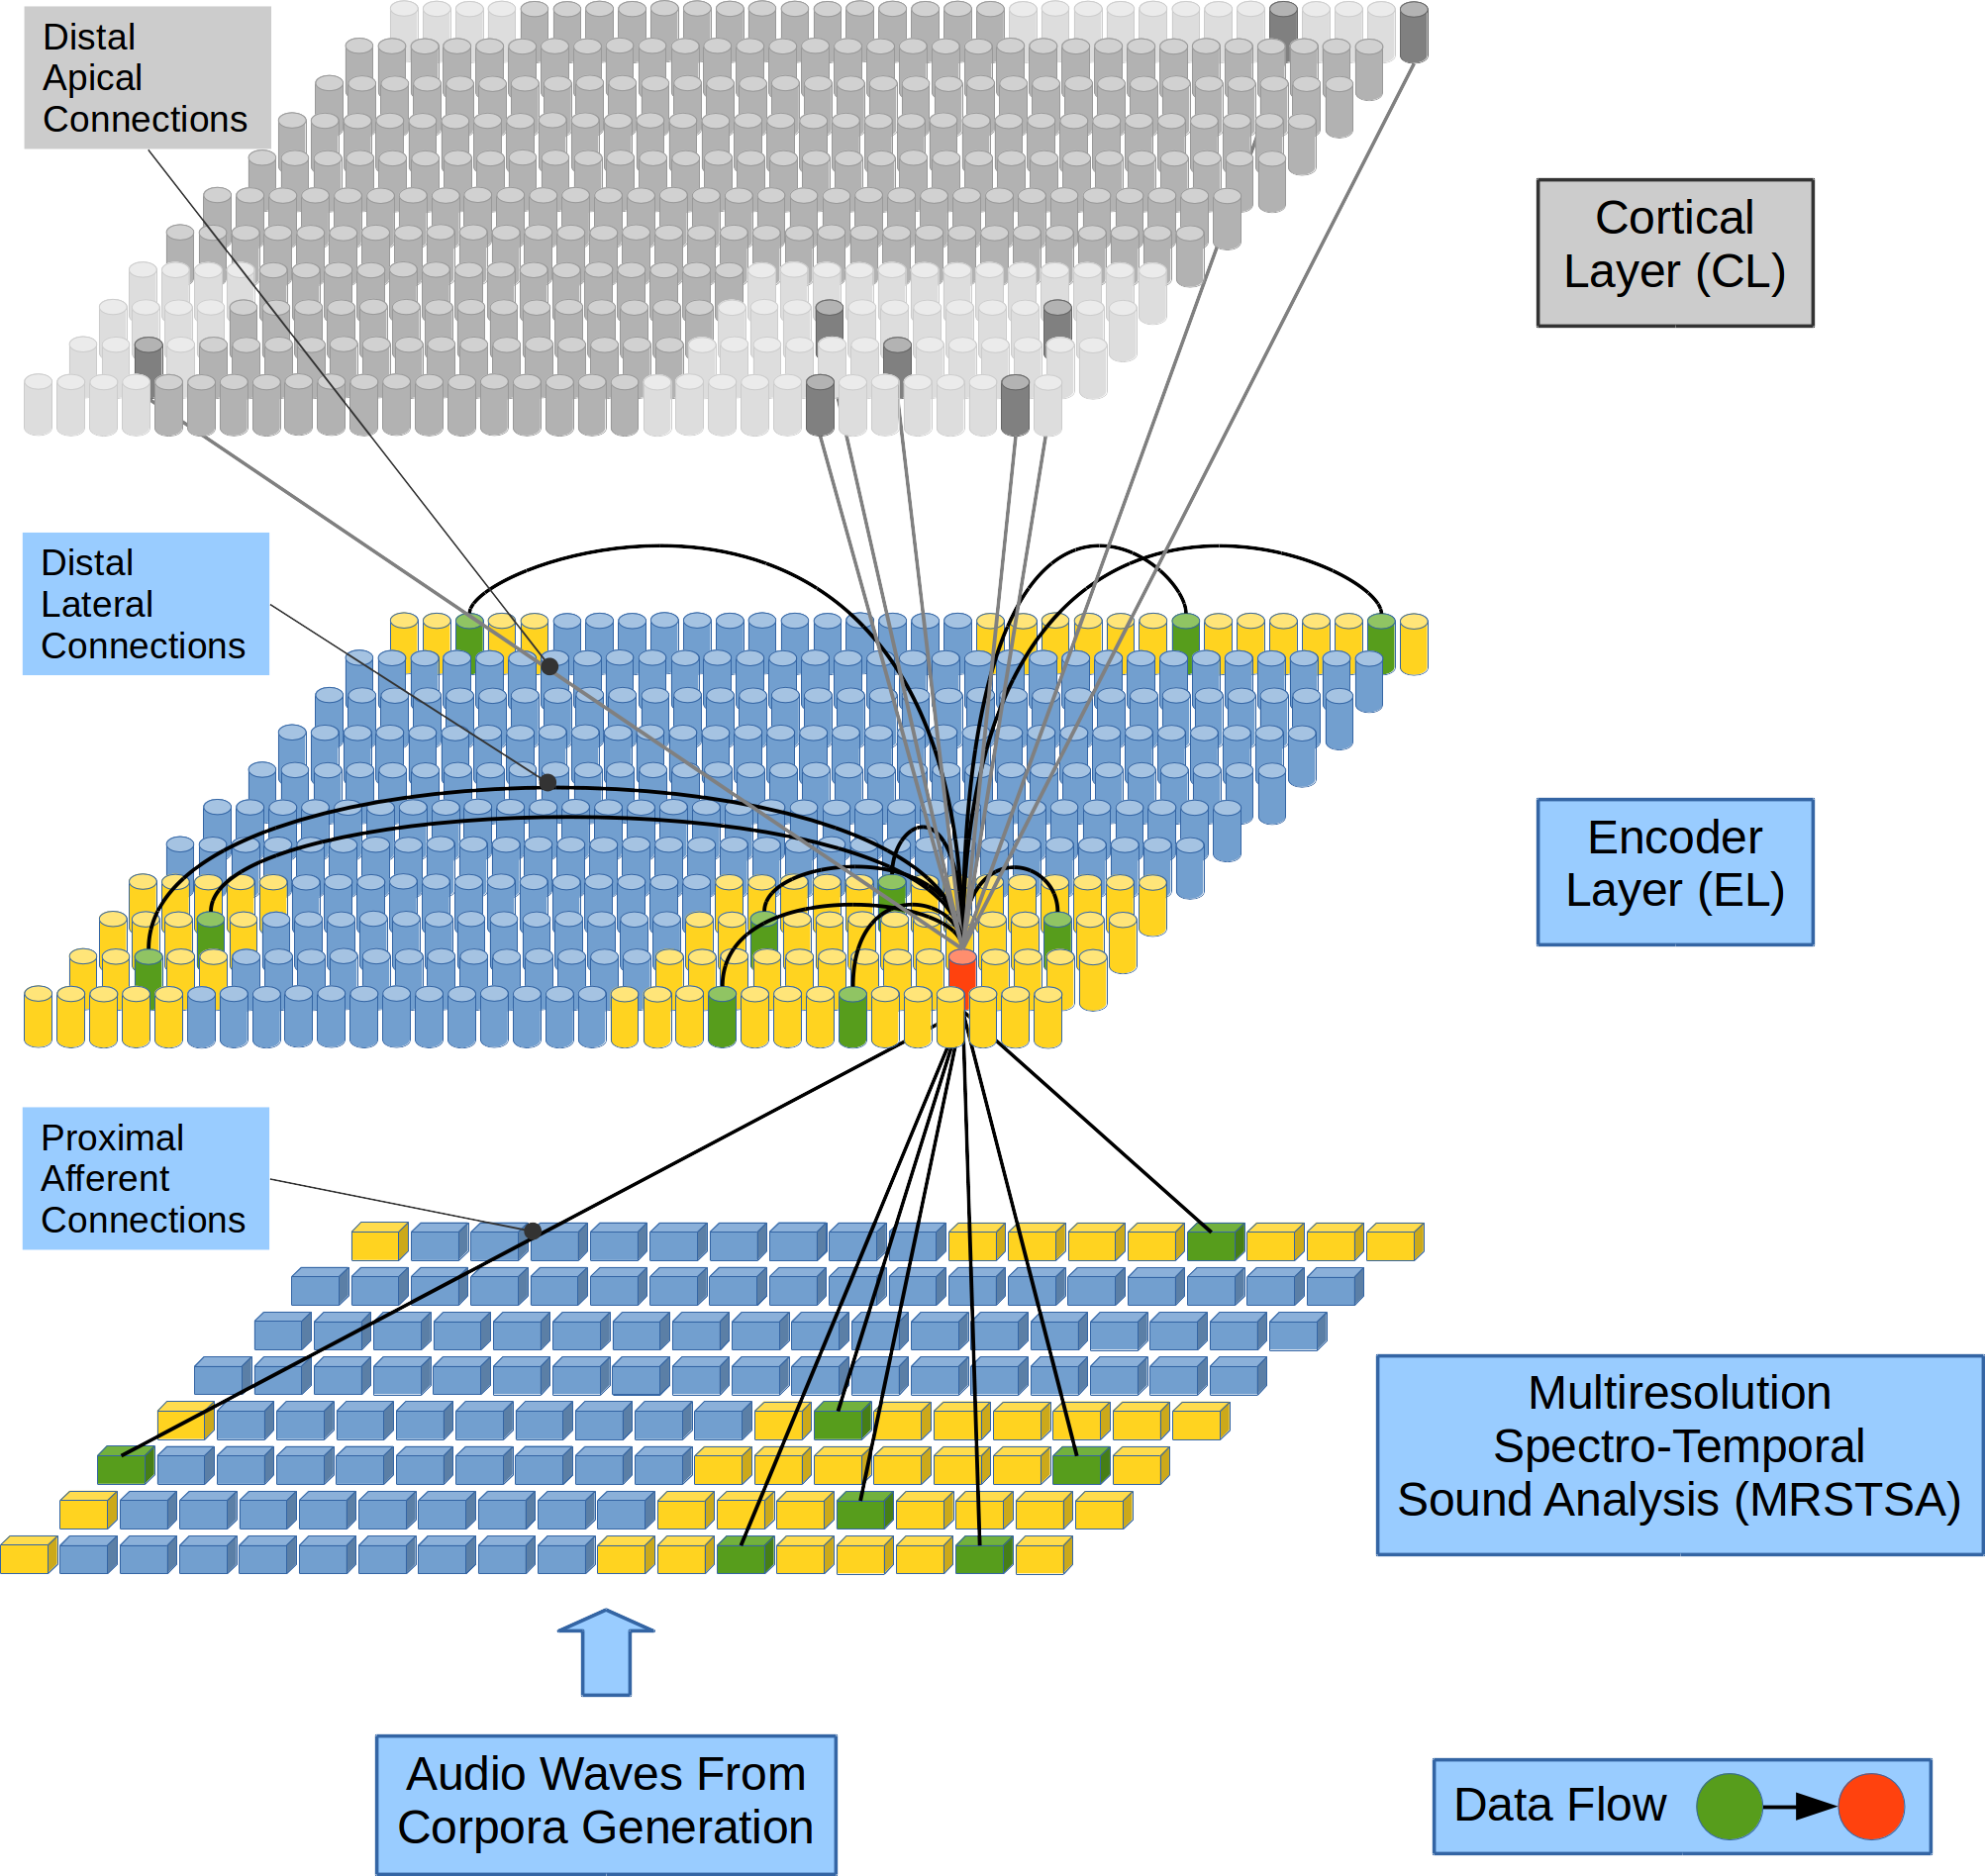
\includegraphics[width=0.7\textwidth]{EncoderColumnConnections1.png}
    \caption{Organización general del \glsfirst{cstm}. Perfil de conectividad dispersa y aleatoria para una \glsfirst{cc} (en rojo) en la \glsfirst{el}.}
    \label{fig:EncoderColumnConnections1}
\end{figure*}

En relación al software para la implementación del modelado computacional, en años recientes, los marcos de \gls{dl} han evolucionado extremadamente rápido y han establecido un territorio de aplicación dinámico.
La primera generación de marcos de \gls{dl}--la cual fue ampliamente adoptada en la comunidad científica--se construyó principalmente en la academia, pero generaciones más recientes se están desviando hacia la industria.
Existe un desvío interesante que da cuenta de los niveles de desarrollo, refinamiento y sofisticación que tales marcos de trabajo pueden ofrecer cuando se comienza a elaborar una implementación de \gls{ai}~\cite{Bahrampour2015ComparativeSO,7979887}.

De hecho, existen tres razones principales que pueden conducir al uso de uno de esos marcos, en lugar de escribir el código de un proyecto desde cero.
La primera razón es que estos marcos habilitan un uso y trato fácil de gráficos computacionales grandes sin tener que preocuparse por los detalles de su manejo.
La segunda razón es que cuando se trabaja en \gls{dl} siempre es necesario computar gradientes, es decir, computar alguna pérdida y luego computar los gradientes alrededor de los pesos con respecto a la pérdida.
Es mejor hacer esas operaciones tan automáticas como sea posible, dejando que la herramienta maneje los detalles del algoritmo \emph{backpropagation}.
Por lo tanto, el escenario común es escribir solo el paso directo de la red y tener el paso reverso de alguna manera libre sin incluir aditamentos significativos al código.
Finalmente, es altamente deseable tener el marco corriendo eficientemente en  \gls{gpu_pl}, sin preocuparse de los detalles del hardware de bajo nivel como los paquetes cuBLAS y cuDNN en \emph{\gls{cuda}}, el movimiento de datos entre la \gls{cpu} y la \gls{gpu}, etc.
De esta manera, los detalles se mantienen ocultos por medio de estas herramientas que los manejan de manera apropiada.

Con estos puntos en mente, se tomaron en cuenta ciertos aspectos para afrontar la implementación de nuestro modelo computacional.
Primeramente, la plausibilidad biológica de  nuestro modelo nos libera de la necesidad de computar gradientes.
Aunque existen trabajos importantes que apoyan la idea de que la asignación de crédito (\emph{credit assignament})--la meta final del algoritmo \emph{backpropagation}--podría ser un fenómeno que sucede en el tejido cortical~\cite{Guerguiev2017TowardsDL}, ponderamos que aún no se sabe si ciertas señales llamadas \emph{teaching signals} existen en el cerebro.
Más aún, no hay suficiente evidencia como para incluir mecanismos tan complejos en nuestro modelo todavía.
En su lugar, decidimos ser conservativos en dicho respecto.
En segundo lugar, los marcos de \gls{dl} están direccionados a la paralelización en \gls{gpu_pl} en núcleos \gls{cuda}.
Más allá de que dichos marcos han sido optimizados extensivamente para sacar el máximo provecho específicamente de las tarjetas NVIDIA, se tienen que satisfacer demasiadas condiciones para obtener el mejor desempeño.
Aunque tales marcos han alcanzado un progreso sobresaliente en los últimos años (junto al desarrollo de su hardware complementario), existe una especialización muy puntual de tales tecnologías hacia el desarrollo preciso de ciertos marcos de \gls{dl} con poco espacio para implementaciones innovadoras y especialmente biológicamente plausibles.
En tal sentido, uno de los mayores problemas en tales enfoques surge cuando se tratan de implementar poblaciones neuronales con estructuras de conectividad dispersa y aleatoria.
Tales implementaciones--fuertemente demandadas en el modelado biológicamente plausible--comprometen la coalescencia en las tarjetas \gls{gpu} y perjudican seriamente el desempeño~\cite{doi:10.3109/0954898X.2012.739292}.

Siguiendo esta línea, implementamos nuestro modelo en \CC14 utilizando el paradigma de \gls{oop} y lo paralelizamos por medio de una estrategia híbrida usando \gls{mpi} y \gls{omp}.
El paradigma de \gls{oop} nos dio una herramienta fuerte para componer estructuras modulares permitiéndonos manejar gráficos computacionales complejos. \gls{mpi} habilitó nuestro modelo para correr en sistemas de memoria distribuida de manera coherente y estable.
Finalmente, \gls{omp} nos proveyó de una distribución fina de la carga de trabajo dentro de cada nodo computacional con la opción de planificar los hilos \gls{omp} de manera dinámica.
Esto nos permitió manejar diferentes opciones de afinidad de hilos y variar el número de hilos en cada nodo computacional, entre otras opciones.
}{
\section{Introduction}

Neuroscience has undoubtedly provided a more in-depth understanding of brain organization in the last decades. Yet, mainstream \gls{ai} research is yet to incorporate these advancements in their models. This fact could be attributed--at least in part--to the success accomplished by some \gls{ai} approaches--such as Deep Convolutional Neural Networks--which have achieved classification accuracy levels without precedent in the last years. Nevertheless, some researchers from the \gls{ai} community recognize that in order to overcome current \gls{ai} limitations and to create intelligent machines it will be necessary to understand and mimic the brain. In such sense, to better understand and explore more deeply how the brain may process information it is essential to use more complex and biophysically accurate neuron and network models than the ones that are prevalent today.

The model of \gls{hh}~\cite{HODGKIN199025}--for example--simulates synaptic receptors and ion channels explicitly. Nevertheless, the more interesting the biological mechanisms, the more limited they are by the size and complexity of the networks. There are some alternative models such as spiking model~\cite{Izhikevich2004SpiketimingDO} and the integrate-and-fire model~\cite{1333071} which have been proposed as a simplification of the \gls{hh} model. Such models demand less computational power, but are not able to directly simulate the biological dynamics present in ion channels. On the other side we find \gls{dl} applications~\cite{lecun_deep_2015} that are partially inspired by the biology of the visual ventral pathway, which have dramatically improved the state-of-the-art in many \gls{ai} domains while ignoring--at the same time--important biological facts and giving priority to computational efficiency and classification accuracy. 

Finding the appropriate level of detail in modeling the brain seems to be the holy grail to disentangle the mysteries of animal behavior. In~\cite{10.1371/journal.pone.0217966} we followed sequence learning mechanisms applied in~\cite{10.3389/fncir.2016.00023} gathering what are--under our point of view--only relevant neuro-anatomical and neuro-physiological facts in order to process information in cortical tissue. In such work we aimed to gather only biologically relevant aspects avoiding loading simulations with excessive computational burden and--at the same time--capturing the essence of the information processing properties in the cortex.

\begin{figure*}[ht]
    \centering
    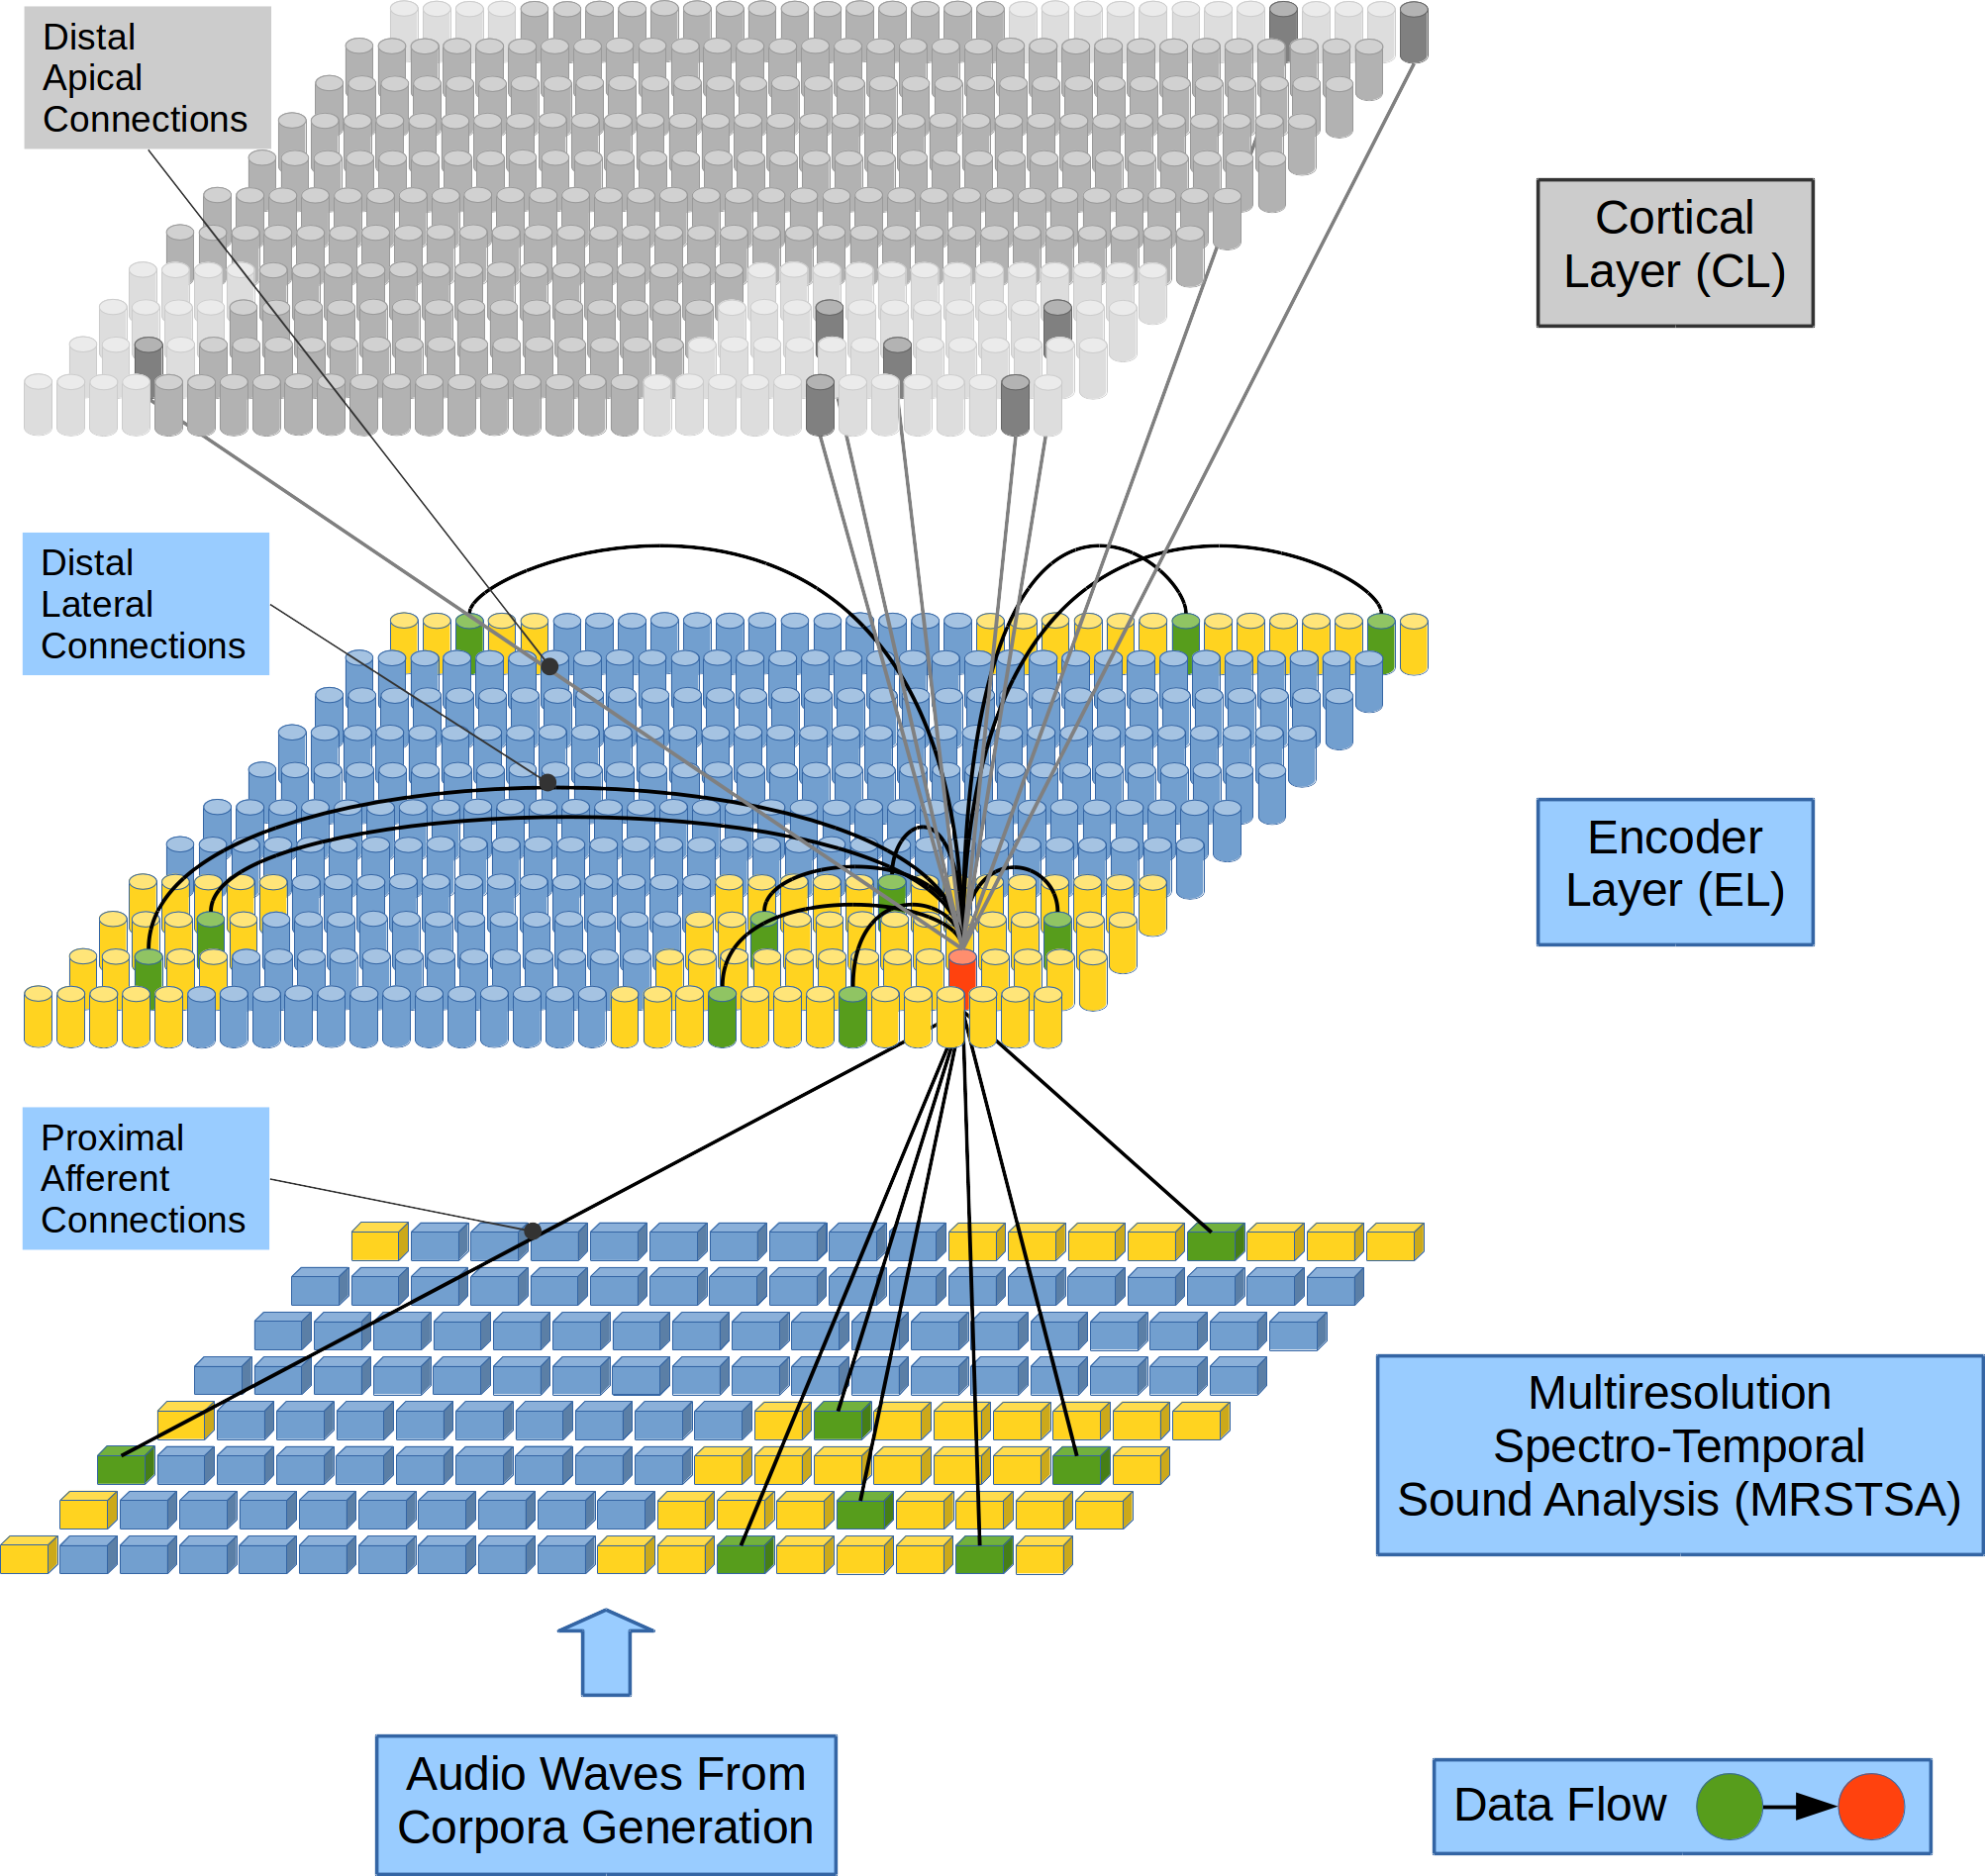
\includegraphics[width=0.7\textwidth]{EncoderColumnConnections1.png}
    \caption{\glsfirst{cstm} general layout. Sparse and random connectivity profile for a \glsfirst{cc} (in red) in the \glsfirst{el}.}
    \label{fig:EncoderColumnConnections1}
\end{figure*}

Regarding software for computational modeling implementation, in recent years, extremely fast evolving and powerful \gls{dl} frameworks have established a dynamic application landscape. The first generation of \gls{dl} frameworks--which was widely adoped in the scientific community--was built mainly in the academia, but the most recent generation is shifting towards the industry. It is an interesting shift  that gives an idea about the level of development, refinement and sophistication that such frameworks could offer when starting a brain model or an \gls{ai} implementation~\cite{Bahrampour2015ComparativeSO,7979887}. 

In fact, there are three main reasons that can lead to the use of one of these frameworks, instead of writing the code from scratch. The first reason is that these frameworks enable to easily deal and work with big computational graphs without worrying about bookkeeping details. The second reason is that when working in \gls{dl} it is always necessary to compute gradients, i.e. to compute some loss and then to compute the gradients about weights with respect to the loss. It is better to make these operations as automated as possible, leaving the framework to handle all backpropagation details. Therefore, the common scenario is to write only the forward pass of the network and have the backward pass rather free without significant additions to the code. Finally, it is highly desirable to have the framework running efficiently on \glspl{gpu}, not worrying about low level hardware details such as cuBLAS and cuDNN packages in \gls{cuda}, moving data between the \gls{cpu} and the \gls{gpu}, etc. In this way, details are kept hidden by these tools that handle them appropriately.

With these points in mind, certain aspects were taken into account in order to pursue the implementation of our computational model. Firstly, the biological plausibility of our model freed us from the need to compute gradients. Even though there are important works supporting the idea that \emph{credit assignament}--the ultimate goal of backpropagation--could be a phenomenon happening in cortical tissue~\cite{Guerguiev2017TowardsDL}, we pondered that it is unknown whether \emph{teaching signals} exist in the brain. Furthermore, there is not enough evidence to include such a complex mechanism in our model yet. Instead, we decided to be conservative in this respect. Secondly, \gls{dl} frameworks are mainly biased towards \gls{gpu} parallelization on \gls{cuda} cores. Albeit those frameworks have been extremely optimized to take the maximum advantage especially from NVIDIA cards, too many conditions have to be satisfied in order to obtain the best performance. Although such frameworks have made an outstanding progress in the last years (together with the development of their complementary hardware), there is an acute specialization of such technologies towards the precise development of certain \gls{dl} frameworks with little room for innovative and specifically biologically plausible implementations. In that sense, one of the biggest problems in such approaches arises when trying to implement neural populations with sparse or random connectivity structures. Those implementations--strongly demanded in biologically plausible modelling--compromise coalescence in \gls{gpu} cards and seriously impairs performance~\cite{doi:10.3109/0954898X.2012.739292}.

Following this line, we implemented our model in \CC14 using \gls{oop} paradigm and parallelized it by means of a hybrid strategy using \gls{mpi} and \gls{omp}. The \gls{oop} paradigm gave us a powerful tool to compose modular structures allowing the management of complex computational graphs. \gls{mpi} enabled our model to run in distributed memory systems in a coherent and stable way. Finaly, \gls{omp} provided a fine grained distribution of  workload inside each computing node with the option to schedule the \gls{omp} threads dynamically. This allowed to manage different options of thread affinity and to vary the number of threads in each computing node, among other options.
}
























\iftoggle{DEBUG}{
\section{Nuestro Aporte}

En este trabajo introducimos una estrategia de paralelización con gran independencia de la coalescencia de datos y mostramos cómo esta escala eficientemente en sistemas de memoria distribuida mientras corre nuestro modelo computacional biológicamente inspirado el cual simula la dinámica cortical con perfiles de conectividad altamente dispersos y aleatorios~\cite{10.1371/journal.pone.0217966}.

La organización general de nuestro enfoque computacional se muestra en la Fig.~\ref{fig:EncoderColumnConnections1}.
En primer lugar, para generar los archivos de audio de los corpus utilizamos el sintetizador Festival \emph{text to speech}~\cite{festival2014}, implementando un código en Python paralelizado por medio de un paquete \gls{mpi} para Python llamado \texttt{mpi4py}.
En segundo lugar, para producir las entradas desde los flujos auditivos seguimos los  lineamientos generales de Chi T. et al.~\cite{chi_2005} e implementamos un algoritmo llamado \glsfirst{mrstsa}~\cite{10.1371/journal.pone.0217966}.
Nuestra implementación sigue principalmente la sección cortical en~T. Chi et al. \cite{chi_2005} en lugar de su contraparte sub-cortical.
Implementamos el algoritmo en C y lo paralelizamos por medio del paradigma híbrido con \gls{mpi} y \gls{omp} utilizando secciones paralelas en \gls{omp}.
Finalmente, en~D. Dematties et al. \cite{10.1371/journal.pone.0217966} nuestro grupo implementó un modelo computacional no supervisado e inspirado biológicamente--la \glsfirst{el} en la Fig.~\ref{fig:EncoderColumnConnections1}--el cual incorpora propiedades claves de la corteza de los mamíferos y devuelve características fonéticas que mejoran los niveles de exactitud en clasificación del algoritmo de \gls{svm} en tareas de clasificación de palabras.
Esto sucede en presencia de ruido, reverberación y variaciones de tono no presentes durante el entrenamiento.
La paralelización del código se lleva a cabo por medio de un paradigma híbrido \gls{mpi} y \gls{omp} y a través del uso de sistemas de archivo paralelos (\gls{mpi} I/O) con capacidad de \emph{Checkpoint} y rearanque en la etapa de entrenamiento donde se tiene total flexibilidad en términos del número de procesos con los que la ejecución es reiniciada. 
Aunque ya implementado, el algoritmo de la \gls{cl} en la Fig.~\ref{fig:EncoderColumnConnections1} todavía no ha sido probado en escalado ni en el desempeño en clasificación fonética.
Decidimos incluir dicha sección en la Fig.~\ref{fig:EncoderColumnConnections1} para mostrar el hecho de que la \gls{el} puede recibir \emph{Conexiones Dendríticas Apicales} desde capas superiores de la misma manera en que recibe \emph{Conexiones Dendríticas Laterales} distales desde \gls{cc_pl} vecinas.

Realizamos todos los experimentos computacionales en Cooley~\cite{noauthor_cooley_nodate}, un cluster para visualización y análisis en el \glsfirst{anl} \footnote{\url{https://www.anl.gov/}} en el cual ejecutamos las siguientes tareas: 
\begin{itemize}
\item Pruebas de escalado para los algoritmos de Generación de Corpus de audio en Python usando hasta 6 nodos corriendo 64 procesos \gls{mpi} sobre 64 \gls{cpu_pl}.
Desempeño en pruebas de escalado Fuerte y Débil. Medidas de eficiencia en escalado.
\item Pruebas de escalado del algoritmo \gls{mrstsa} utilizando hasta 64 nodos (un proceso \gls{mpi} por nodo) y hasta 5 hilos \gls{omp} por nodo/proceso.
Pruebas de desempeño en escalado Fuerte y Débil. Mediciones de eficiencia en escalado. 
\item Pruebas de escalado en la \gls{el}--el algoritmo central de nuestro modelo--utilizando hasta 64 nodos (un proceso \gls{mpi} por nodo) y hasta 8 hilos \gls{omp} por nodo/proceso. Realizamos pruebas de escalado Fuerte y Débil y medimos eficiencia de escalado.
\end{itemize}

Las medidas de eficiencia de escalado devueltas por nuestras pruebas nos permiten vislumbrar un uso eficiente de recursos computacionales paralelos de alto desempeño.
En este trabajo hemos mostrado un enfoque de paralelización viable para implementaciones altamente flexibles de modelos corticales cerebrales en los que la coalescencia de los datos no es un requisito fundamental.
Hemos mostrado la versatilidad de este esquema de paralelización en nuestro modelo computacional inspirado en el cerebro simulando la dinámica cortical con un perfil de conexión altamente disperso y aleatorio.
De esta forma podemos decir que esta estrategia de paralelización es un procedimiento prometedor para abordar nuevas implementaciones computacionales, con más plausibilidad biológica y con conjuntos de datos más irregulares y desestructurados en recursos computacionales de alto desempeño.
}{
\section{Our Contributions}

In this paper we introduce a parallelization strategy with great independence on data coalescence and show how it scales efficiently on distributed memory systems while running our biologically-inspired computational model which simulates cortical dynamics with highly sparse and random connectivity profiles~\cite{10.1371/journal.pone.0217966}.

The general layout of our computational setup is shown in Fig.~\ref{fig:EncoderColumnConnections1}. First, to generate the corpora audio files, we employed Festival text to speech synthesizer~\cite{festival2014}, implementing a Python code parallelized by means of a \gls{mpi} package for Python called mpi4py. Second, in order to produce the inputs from auditory streams we followed main guidelines from Chi T. et al.~\cite{chi_2005} and implemented an algorithm called \gls{mrstsa}~\cite{10.1371/journal.pone.0217966}. Our implementation follows primarily the cortical section in~\cite{chi_2005} rather than its sub-cortical counterpart. We implemented the algorithm in C and parallelized it by means of \gls{mpi} and \gls{omp} hybrid paradigm using \gls{omp} parallel sections. Finally, in~\cite{10.1371/journal.pone.0217966} our group pursued the implementation of a completely unsupervised and biologically inspired computational model--the \glsfirst{el} in Fig.~\ref{fig:EncoderColumnConnections1}--which incorporated key properties from the mammalian cortex and returned phonetic features that improved the classification accuracy levels of the \gls{svm} algorithm in word classification tasks. This happened in the presence of noise, reverberation and pitch variations not present during training. The parallelization of the code is approached by means of a hybrid \gls{mpi} and \gls{omp} paradigm and through the use of \gls{mpi} I/O parallel file system with Checkpoint and Restart capacity in the training stage where there is total flexibility in terms of the number of ranks with which the execution is restarted. While already implemented, the \gls{cl} algorithm in Fig.~\ref{fig:EncoderColumnConnections1} has not yet been tested in scaling nor in phonetic classification performance. We decided to sketch it in Fig.~\ref{fig:EncoderColumnConnections1} to show the fact that \emph{Distal Apical Connections} from superior layers can be received by the \gls{el} in the same fashion than \emph{Distal Lateral Connections} from neighboring \glspl{cc}. 

We performed all computational experiments on Cooley~\cite{noauthor_cooley_nodate}, a visualization and analysis cluster at Argonne National Laboratory in which we executed the following tasks: i) scaling tests on audio Corpora Generation algorithm in python using up to 6 nodes running 64 \gls{mpi} processes on 64 \glspl{cpu}. Performance of strong and weak scaling tests. Measurement of scaling efficiency. ii) scaling tests on the \gls{mrstsa} algorithm using up to 64 nodes (one \gls{mpi} rank per node) and up to 5 \gls{omp} threads per node/rank. Performance of strong and weak scaling tests. Measurement of scaling efficiency. iii) scaling tests on the \gls{el}--the central algorithm in our model--using up to 64 nodes (one \gls{mpi} rank per node) and up to 8 \gls{omp} threads per node/rank. We performed strong and weak scaling tests and measure scaling efficiency. 

The measurements of scaling efficiency returned by our tests allow us to foresee an efficient use of high-end parallel computing resources. In this paper we have shown a viable parallelization approach for highly flexible implementations of cortical brain models in which data coalescent is not a tight requirement. We have shown the versatility of this parallelization scheme on our brain-inspired computational model of cortical dynamics with a random and a highly sparse connection profile. In this way we can claim that this parallelization strategy is a promising procedure to approach new computational implementations, with more biological plausibility and with more irregular and unstructured data-set in high-end leadership computer resources.
}



















\iftoggle{DEBUG}{
\section{Trabajo Relacionado}

Más allá de que el cerebro de los humanos consume alrededor de 25 Watts~\cite{edited_by_stephen_c._cunnane_human_2010}, este tiene en promedio 86 billones de neuronas~\cite{Azevedo2009EqualNO} y trillones de sinapsis ya que cada neurona se conecta con otras neuronas utilizando miles de vínculos sinápticos.
Cada sinapsis puede computar una operación en 0.005 segundos dando al cerebro humano la capacidad de computar 20 billones de operaciones por segundo~\cite{10.2307/j.ctt5vkr1h}.
Aunque tales números parecen arrolladores, dicha capacidad de computación es aún mejorada por medio de propiedades únicas existentes en el tejido cortical, tales como una gran tolerancia a fallas, una flexibilidad exhaustiva y un alto nivel de paralelismo.

El esfuerzo computacional demandado por tales especificaciones nos obliga  a considerar sólo aquellas características fisiológicas y anatómicas claves para el procesamiento de la información en el cerebro, evitando así cargar las simulaciones computacionales con detalles biológicos innecesarios.
En la misma dirección, las estrategias de paralelización tienen que ser altamente efectivas para afrontar los desafíos presentados por la implementación de enfoques nuevos y biológicamente precisos en recursos \gls{hpc}.

}{
\section{Related Work}

In spite of the fact that the human brain consumes around 25 Watts~\cite{edited_by_stephen_c._cunnane_human_2010}, it has on average 86 billions neurons~\cite{Azevedo2009EqualNO} and trillions of synapses since each neuron connects to other neurons using thousands of synaptic links. Each synapse can compute one operation on 0.005 seconds giving the human brain the capacity to compute about 20 billion operations per second~\cite{10.2307/j.ctt5vkr1h}. Even though such numbers seems overwhelming, this computing capacity is still enhanced by means of unique properties existent in brain tissue such as impressive fault and noise tolerance, exhaustive flexibility and high level of parallelization.

The computational effort demanded by such specifications force us to consider only those physiological and anatomical features which are key for information processing in the brain avoiding loading computational simulations with unnecessary biological detail. In the same direction, parallelization strategies have to be as highly qualified as to face the challenges presented by the implementation of new--biologically accurate--computational approaches on~\gls{hpc} resources.

}








\iftoggle{DEBUG}{
\subsection{Enfoques Computacionales de \gls{ann_pl} Inspiradas en el Cerebro}

Una de las principales motivaciones del modelo inspirado en el cerebro es desarrollar nuevos algoritmos más poderosos cuya inspiración en el cerebro nos permita procesar la información de una manera más efectiva y eficiente para construir sistemas con comportamientos más inteligentes.

El desarrollo de las \gls{ann_pl} se clasifica en tres generaciones en relación a sus unidades computacionales~\cite{MAASS19971659,10.1007/978-3-642-03156-4_17}.
En 1943, la primer generación de \gls{ann_pl} vino de la mano de McCulloch y Pitts~\cite{McCulloch1990ALC}.
Los autores introdujeron neuronas como unidades computacionales que recibían entradas binarias asociadas a pesos y producían salidas binarias dependientes de un umbral.
Derivaciones importantes de tales \gls{ann_pl} son los perceptrones multicapa, las redes de Hopfield y las Máquinas de Boltzman.

En la segunda generación, las unidades neuronales son elementos computacionales cuyas salidas representan un conjunto continuo de valores posibles por medio de funciones de activación aplicadas a la suma ponderada de las entradas.
Funciones de activación comunes son la sigmoide, la polinomial o la exponencial.
Ejemplos de dichas redes son las redes neuronales sigmoidales de vía directa (\emph{feedforward}) y recurrentes. 
Un rasgo extremadamente importante de tales redes es que sostienen algoritmos de aprendizaje basados en descenso de gradiente (\emph{gradient descent})--como el popular \emph{backpropagation}.
Finalmente, las salidas de valores reales de la neuronas de esta generación se interpretan como tasas de disparo en las neuronas reales.

Importante evidencia comportamental y fisiológica, sin embargo, puso en duda la \emph{interpretación de la tasa de disparo}, y dio lugar a la tercera generación de \gls{ann_pl} que emplearon \emph{neuronas de impulso} (\emph{spiking neurons})--o \emph{neuronas de integración y disparo} (\emph{integrate and fire neurons})--como unidades computacionales~\cite{HODGKIN199025,Izhikevich2004SpiketimingDO,1333071}.
Estos modelos--a diferencia de los modelos de la segunda generación--utilizan temporización con potenciales de acción--o disparos--para codificar la información.
Incluyendo el concepto de tiempo en su modelo de procesamiento, las \gls{snn_pl} pudieron capturar el comportamiento neuronal de manera más precisa que las redes neuronales tradicionales.
A diferencia de las \gls{ann_pl} la idea principal es que las neuronas en una \gls{snn} no disparan en cada ciclo, en su lugar, lo hacen sólo si un potencial de membrana alcanza su umbral.

Independientemente de que este enfoque de modelado es convincente, los circuitos de umbral como los introducidos en la primera generación pueden ser vistos como modelos abstractos de computación digital sobre redes de neuronas de impulso.
En tal sentido, un bit en estado activo se podría interpretar como una neurona disparando dentro de cierta ventana corta de tiempo y el mismo bit en estado inactivo se podría interpretar como la misma neurona no disparando en tal ventana~\cite{Valiant:1994:CM:199266}.
Esta estrategia de codificación provee un buen modelo para una red de neuronas de impulso, siempre y cuando los tiempos entre las neuronas pre y post-sináptica estén sincronizados dentro de ventanas de tiempo de pocos milisegundos.
Existe evidencia que sostiene el hecho de que dicha actividad fuertemente sincronizada realmente ocurre en el tejido biológico~\cite{Abeles1993SpatiotemporalFP,bair1994}.

En tal sentido, existen nuevos desarrollos algorítmicos~\cite{10.3389/fncir.2016.00023,10.1371/journal.pone.0217966} que en lugar de modelar activaciones precisamente temporizadas priorizan los diferentes roles de las configuraciones dendríticas próximas y distales incorporando fenómenos fisiológicos y anatómicos importantes como la consideración de las ramas dendríticas como elementos de procesamiento activos, la organización columnar en el tejido cortical y los patrones de activación dispersos en el neocortex--entre otros.
Casi todas las \gls{ann_pl}, como aquellas utilizadas en aprendizaje profundo~\cite{lecun_deep_2015} y redes neuronales de impulso~\cite{MAASS19971659}, usan neuronas sin considerar dendritas activas y con un número no realista--muy bajo--de sinapsis.
Estos hechos sugieren que esas \gls{ann_pl} están perdiendo propiedades funcionales fundamentales presentes en el tejido del cerebro.
}{
\subsection{Brain-Inspired \gls{ann} Computational Approaches}

One of the main motivations of brain-inspired modeling is to develop new and more powerful algorithms whose inspiration in the brain allows us to process the information better in order to forge systems with more intelligent behaviors.

The development of~\glspl{ann} is classified in three generations regarding their computational units~\cite{MAASS19971659,10.1007/978-3-642-03156-4_17}. In 1943, the first generation of~\glspl{ann} came from McCulloch and Pitts~\cite{McCulloch1990ALC}. The authors introduced neurons as computational units which received binary inputs through associated weights and produced threshold dependent binary outputs. Important derivations from such~\glspl{ann} are multilayer perceptrons, Hopfield nets and Boltzman Machines.

In the second generation, neural units are computational elements whose outputs represent a continuous set of possible values obtained by means of activation functions applied to the weighted sum of the inputs. Common activation functions are sigmoid, polynomial or exponential functions. Examples of these networks are feedforward and recurrent sigmoidal neural nets. An extremely important feature of these networks is that they support learning algorithms based on gradient descend--such as the popular backpropagation. Finally, the real-valued outputs of networks of this generation are interpreted as firing rates in real neurons. 

Important behavioral and physiological evidence though made \emph{firing rate interpretation} questionable, and gave rise to the third generation of \glspl{ann} which employ \emph{spiking neurons}--or \emph{integrate and fire neurons}--as computational units~\cite{HODGKIN199025,Izhikevich2004SpiketimingDO,1333071}. These models--unlike the second generation models--use timing of single action potential--or spikes--to encode information. Including the concept of time in their processing model,~\glspl{snn} could capture neural behavior more accurately than traditional neural networks. Unlike traditional \glspl{ann}, the main idea is that neurons in a~\gls{snn} do not fire at each cycle, and rather they fire only if a membrane potential reach its threshold.

In spite of such compelling modeling approach, threshold circuits like the ones introduced by the first generation could be seen as abstract models for digital computation on networks of spiking neurons. In such sense, one bit in active state could be interpreted as a neuron firing within certain short time window and the same bit in inactive state could be interpreted as the same neuron non-firing within such time window~\cite{Valiant:1994:CM:199266}. This coding strategy provides a good model for a network of spiking neurons as long as firing times among pre and postsynaptic neurons are synchronized within a few msec time window. There is evidence supporting the fact that this strongly synchronized activity does really occur in biological tissue~\cite{Abeles1993SpatiotemporalFP,bair1994}.

In such sense, there are new algorithmic developments~\cite{10.3389/fncir.2016.00023,10.1371/journal.pone.0217966} which instead of modeling precise timing activations prioritize the different roles of proximal and distal dendritic configurations incorporating important physiological and anatomical phenomena such as the consideration of dendritic branches as active processing elements, the microcolumnar organization in cortical tissue and the sparse patterns of activation in the neocortex--among others. Almost all \glspl{ann}, such as those used in deep learning~\cite{lecun_deep_2015} and spiking neural networks~\cite{MAASS19971659}, use artificial neurons without considering active dendrites and with an unrealistic low number of synapses. These facts suggest that those \glspl{ann} are missing fundamental functional properties present in brain tissue. 
}










\iftoggle{DEBUG}{
\subsection{\glspl{cpu} y \glspl{gpu} para Simulaciones Grandes de \gls{ann_pl}}

Los objetivos de diseño originales de las \gls{cpu_pl} estaban principalmente direccionados a hacer a los hilos individuales muy rápidos, reduciendo la latencia por medio de sistemas grandes de cache y ejecución especulativa incluyendo predicción de ramificaciones y de dependencia de memoria en los procesadores con sistemas de \emph{pipeline}.
En contraste, para las \gls{gpu_pl} el rendimiento general es más importante que los hilos individuales y en dichos dispositivos la latencia de la memoria se oculta por medio de paralelismo masivo evitando así los relojes de alta frecuencia presentes en las \gls{cpu_pl}.

Esencialmente, cada operación en una \gls{gpu} es paralela. En una \gls{cpu} en cambio, el compilador tiene que ser persuadido de que una operación se puede vectorizar.
Para lograr esto, la operación en la \gls{cpu} tiene que satisfacer algún criterio, por ejemplo, los datos utilizados por la operación tienen que estar alineados en memoria de cierta manera--esta es una restricción importante.
Cada operación en una \gls{gpu} es vectorizada (sin alternativa) y no hay ninguna necesidad de persuadir al compilador para realizar operaciones vectoriales en una \gls{gpu}.
Por lo tanto, cada núcleo \gls{cpu} ejecuta operaciones escalares o vectoriales mientras que cada núcleo \gls{gpu} ejecuta sólo instrucciones vectoriales.
De todas maneras, este acceso irrestricto a la vectorización no viene de manera gratuita, ya  que la coalescencia es un requerimiento fuerte para obtener mediciones de alta eficiencia paralela sobre las \gls{gpu_pl}.

En referencia al mercado de las \gls{gpu_pl} y su relación con las aplicaciones de \gls{dl}, NVIDIA--a diferencia de AMD--ha invertido mucho en los últimos años para el \gls{dl}.
Mucho esfuerzo de ingeniería se ha invertido por NVIDIA para hacer su hardware más adecuado al \gls{dl}.
Como ejemplo de ello podemos citar los últimos núcleos (\emph{tensor cores}) de Volta los que pueden realizar una operación  de matrices de 4 por 4 $A*B+C$ completamente en paralelo.
Como resultado, NVIDIA es muy dominante en lo que respecta al \gls{dl} actualmente.

En el reino de los modelos computacionales biológicamente plausibles, la dicotomía \gls{cpu}/\gls{gpu} no está tan claramente definida como en el \gls{dl}.
En~H. Ülo Dinkelbach et al. \cite{doi:10.3109/0954898X.2012.739292} por ejemplo, los autores analizaron las ventajas y desventajas de la paralelización en \gls{cpu} y \gls{gpu} en diferentes paradigmas de paralelización de memoria compartida, como \gls{omp}, \gls{cuda} y \emph{\gls{opencl}} de neuronas de tasa de disparo medio.
Los autores probaron diferentes limitadores de velocidad como la precisión del punto flotante, la configuración de hilos, la organización de los datos y la estructura de conectividad de las redes.
Las implementaciones paralelas en \gls{cpu} fueron muy beneficiadas con redes más pequeñas, mayormente por los efectos de la cache.
Las redes grandes--en cambio--se beneficiaron con las \gls{gpu_pl} solo si estas demandaban memoria más allá de la disponible en las caches de las \gls{cpu_pl}, de lo contrario la implementación en \gls{omp} fue altamente preferida.
Los autores compararon varias representaciones estructurales sobre marcos de paralelización diferentes mostrando que en las \gls{cpu_pl}, dichas representaciones alcanzaban casi el mismo tiempo de computación; en las \gls{gpu_pl} en cambio, el desempeño se vió seriamente afectado por las violaciones de coalescencia inducidas por estructuras de datos heterogéneas.
Finalmente, el problema más serio apareció cuando la red presentó una estructura de conectividad dispersa y aleatoria, es decir, cuando las neuronas recibían conexiones aleatoriamente desde otras neuronas, y no en un orden ascendentemente organizado.
Como explicaron los autores, esto destruyó por completo el desempeño de las implementaciones en \gls{gpu_pl}, mientras que las \gls{cpu_pl} fueron levemente afectadas.
Este fue quizás el argumento más fuerte en contra de las implementaciones en \gls{gpu_pl} de redes neuronales de tasa media de disparo, ya que la conectividad dispersa es un patrón repetitivo en las redes biológicas así como lo es en el modelo computacional presentado en este trabajo.

En~ J. Vitay et al. \cite{10.3389/fninf.2015.00019} los autores describieron un simulador neuronal que provee inferencia de alto nivel para generar redes neuronales con codificación de tasa de disparo, codificación de disparo o red híbrida.
Las definiciones de las redes generan una librería en \CC altamente optimizada para un marco de paralelización subyacente tal como \gls{omp} para sistemas de memoria compartida o \gls{cuda} para \gls{gpu_pl}.
Para la implementación en \gls{omp}, se varío el número de hilos entre 2 y 12.
Para la implementación en \gls{cuda}, se utilizó la configuración por defecto del simulador (32 hilos las actualizaciones de las variables neuronales, 192 hilos para las sumas ponderadas).
Con \gls{omp}, el escalado para 1000 neuronas fue ligeramente subóptimo, mientras que el de 4000 neuronas se saturó rápidamente.
La situación se revirtió con \gls{cuda}.
En tal caso la red con 1000 neuronas solo alcanzó una tasa de aceleración limitada, mientras que la red con 4000 neuronas alcanzó una gran tasa.

En~A. A. Huqqani et al. \cite{HUQQANI2013349} los autores desarrollaron y analizaron dos estrategias de paralelización diferentes para redes neuronales con \emph{backpropagation} para reconocimiento de rostros.
El trabajo se concentró en dos ambientes de paralelización.
Por un lado, se utilizó \gls{omp} sobre una \gls{cpu} multi-hilo convencional y por el otro lado se utilizó \gls{cuda} sobre una \gls{gpu}.
Los autores concluyeron que la paralelización basada en \gls{gpu} se debía de preferir generalmente frente a la basada en \gls{cpu} con múltiples hilos.
Sin embargo, para simulaciones con entradas pequeñas y para un número pequeño de neuronas ocultas, la ejecución basada en \gls{cpu} fue la superior.

En este escenario encontramos un patrón recurrente en el cual las redes neuronales más grandes son beneficiadas por \gls{cuda} mientras que las redes más pequeñas se benefician con \gls{omp}.
Sin embargo, es importante considerar factores clave tales como la irregularidad, dispersión y aleatoriedad de las estructuras de conectividad de la red en el contexto de su relación con la coalescencia de datos en la eficiencia de paralelización.
}{
\subsection{\glspl{cpu} and \glspl{gpu} for \gls{ann} Large Simulations}

Original design goals on \glspl{cpu} were mainly directed towards making single threads very fast by means of reducing latency through large cache systems and speculative execution including branch and memory dependence prediction in pipelined processors. In contrast, for \glspl{gpu} throughput matters more than single threads, hiding memory latency through massive parallelism and avoiding in this way the high frequency clock speeds present in \glspl{cpu}.

Essentially, every operation on a \gls{gpu} is parallel. On a \gls{cpu} instead, the compiler has to actually be persuaded that an operation can be vectorized. In order to do that, the operation on the \gls{cpu} has to satisfy some criteria, for example, the data used for the operation has to be aligned in memory in a certain way. This is an important restriction. At the core level every operation on a \gls{gpu} is vectorized (without alternative). There is no need of persuading the compiler in order to make vector operations on a \gls{gpu}. Then each \gls{cpu} core executes scalar or vector operations while each \gls{gpu} core only executes vector instructions. Nevertheless, the easily accessed vectorization is not for free, since coalescence is a strong requirement to get high parallel efficiency measurements on \glspl{gpu}.

In reference to \gls{gpu} market and its relationship to \gls{dl} applications, NVIDIA--unlike AMD--has been pushing a lot in the last years for \gls{dl}. A lot of engineering effort has been invested by NVIDIA to make their hardware better suited for \gls{dl}. As an example of that we can cite the last Volta tensor cores which can do an $A*B+C$ 4 by 4 matrix operation completely in parallel. As a result NVIDIA is pretty dominant in \gls{dl} currently.

In the realm of biologically plausible computational models the \gls{cpu}/\gls{gpu} dichotomy is not as clearly defined as in \gls{dl}. In~\cite{doi:10.3109/0954898X.2012.739292} for example, the authors analyzed the advantages and drawbacks of the \gls{cpu} and \gls{gpu} parallelization in different shared memory parallel paradigms, such as \gls{omp}, \gls{cuda} and \gls{opencl} of mean-firing rate neurons. The authors inspected different speed limiters such as floating point precision, thread configuration, data organization and connectivity structure of the networks. Parallel \gls{cpu} implementations greatly benefited smaller networks, mostly because of cache effects. Large networks--on the other hand--benefited from the \gls{gpu} only if they demanded memory beyond the available on \gls{cpu} caches, otherwise an \gls{omp} implementation was highly preferred. The authors compared several structure representations on the different parallel frameworks showing that on \glspl{cpu}, these representations reached almost the same computation time, on \glspl{gpu} instead, the performance was significantly affected by violations of coalescence induced by heterogeneous data structures. Finally, the most serious problem appeared when the network had a sparse or random connectivity structure, i.e. neurons received connections randomly from other neurons, and not in an organized or ascending order. As the authors pointed out, this totally broke down the performance of \gls{gpu} implementations, while \gls{cpu} were slightly affected. This was maybe the strongest argument against \gls{gpu} implementations of mean-firing rate neural networks, since this sparse connectivity is a repeated pattern in biological networks as well as it is in the computational model presented in this paper.

In~\cite{10.3389/fninf.2015.00019} the authors described a neural simulator that provides a high-level interface to generate rate-coded, spike-coded or hybrid neural networks. The definitions of the networks generate a \CC~library highly optimized for an underlying parallel framework such as \gls{omp} for shared memory systems or \gls{cuda} for \glspl{gpu}. For the \gls{omp} implementation, the number of threads was varied between 2 and 12. For the \gls{cuda} implementation, the default configuration of the simulator (32 threads for the neural variables updates, 192 threads for the weighted sums) was used. With \gls{omp}, the scaling for 1000 neurons was slightly sub-optimal, while the one for 4000 neurons saturated quickly. The situation was reversed with \gls{cuda}. In such case the network with 1000 neurons only achieved a limited speedup ratio, while the network with 4000 neurons achieved a high ratio.

In~\cite{HUQQANI2013349} the authors developed and analyzed two parallel training strategies for backpropagation neural networks for face recognition. This work concentrated on two parallelization environments. On the one hand, \gls{omp} was used on a conventional multithreaded \gls{cpu} and on the other hand \gls{cuda} was used on a \gls{gpu}. The authors concluded that \gls{gpu} based parallelization should be preferred generally to \gls{cpu} based multithreaded program. However, for some simulations with small input and few hidden neurons \gls{cpu} based execution was better.

In this scenario we find a recurrent pattern in which larger networks are benefited from \gls{cuda} while smaller ones are benefited from \gls{omp}. Nevertheless, it is very important to consider key factors such as irregularity, sparseness and randomness of data structures and network connectivity in the context of its relationship with data coalescence in parallel efficiency.
}









\iftoggle{DEBUG}{
\subsection{Multi-Hilo y Multi-Proceso para Implementaciones Paralelas de \gls{ann_pl} en Sistemas de Memoria Compartida}

Desde un punto de vista teórico, sobre un solo nodo de memoria compartida no hay necesidad de generar redundancia de \emph{código} ni del \emph{heap} ya que están disponibles para ser accedidos libremente.
Por otro lado, los \emph{registros}, el \emph{contador de programa} y la \emph{pila} deben ser replicados para establecer un contexto coherente para cada hilo de ejecución.
De esta manera, la paralelización con multi-hilos debería preferirse sobre la paralelización con multi-procesos en un sistema de memoria compartida.
En implementaciones con \gls{omp}--por ejemplo--los hilos computan diferentes partes de las redes en paralelo.
Debido a que la memoria se comparte entre los hilos, cada uno accede a los datos de los otros hilos libremente.
Por lo dicho, tanto la computación interna de la red así como el tráfico de datos  se llevan a cabo localmente.
Sin embargo, la coherencia de la caché produce sobrecargas adicionales que son más pronunciadas cuando se corren redes pequeñas y se crea un excesivo número de hilos.
Las implementaciones que usan \gls{mpi} habilitan el intercambio de datos entre núcleos sobre memoria compartida en un nodo.
En cada núcleo, una unidad de ejecución única--un proceso \gls{mpi}--maneja un subconjunto de redes neuronales y se comunica con otros procesos usando métodos \gls{mpi} especiales.
En algunos casos la mayor carga de \gls{ipc} se compensa con la ausencia del fenómeno denominado \emph{false-shearing} entre hilos \gls{omp}.
En una implementación híbrida, los núcleos se organizan frecuentemente en grupos--como procesos \gls{mpi}.
Dentro de cada grupo, todos los núcleos se comunican sobre memoria compartida, corriendo hilos \gls{omp} para acelerar la tarea.
En cada grupo, un hilo--el maestro--puede realizar llamadas \gls{mpi} de un solo hilo para intercambio de datos inter-grupo, mientras que el empaquetado y desempaquetado de los datos puede ser realizado por los hilos \gls{omp} generados por el grupo completo.
Este tipo de implementación es una solución de compromiso agrupando ventajas de desventajas de ambas estrategias, la cual es lógicamente extensible a plataformas multi-nodo.

Olena Schuessler y Diego Loyola~\cite{Schuessler:2011:PTA:1997052.1997062} delinearon diferentes métodos para la paralelización de redes neuronales artificiales basadas en el algoritmo \emph{backpropagation} utilizando multihilado y \gls{cpu_pl} multinúcleo en un sistema de memoria compartida.
En este trabajo, los autores usaron Hilos \gls{posix} (Pthreads) y \gls{omp} obteniendo un incremento en velocidad de cómputo muy cercano al ideal esperado (743\% utilizando 8 núcleos).
El entrenamiento paralelo implementado en \gls{omp} devolvió resultados ligeramente mejores comparados a los Pthreads.

En~A. Strey \cite{Strey2003ACO}, se comparó una implementación basada en hilos sobre \gls{omp} con una implementación basada en procesos sobre \gls{mpi} en una arquitectura rápida de memoria compartida.
Se exploraron diferentes estrategias de particionado de datos como así también el desempeño de todas las implementaciones.
Se mostró que las implementaciones basadas en \gls{mpi} fueron significativamente más rápidas que las basadas en \gls{omp}.
Los autores señalaron que la aceleración más baja de la implementación basada en \gls{omp} pareció ser originada en el fenómeno denominado \emph{cache line false sharing} de los arreglos de datos. Tal situación puede ser revertida utilizando varias configuraciones de números de hilos en diferentes corridas.

En~B. P. Gonzalez et al. \cite{6232827} los autores propusieron usar \gls{mpi} y \gls{omp} en un enfoque de \gls{eann} para \gls{tsf} basado en un \gls{eda} que evoluciona una red \gls{eann} completamente conectada (\emph{fully connected}).
Los experimentos utilizaron varias series temporales y el número de núcleos se extendió de 1 a 6.
De esta forma los autores mostraron que \gls{mpi} con 5 núcleos fue la mejor estrategia de paralelización, la cual tomó el menor tiempo de ejecución e hizo un uso razonable de los recursos computacionales.

En~M. Joldos y I. L. Muntean \cite{6511739} los autores reportaron una paralelización basada en \gls{omp} para la implementación de un simulador de \gls{snn} asíncrono con el objetivo de mostrar eficiencia básica de paralelización de núcleo y de hiper-hilado.
Los primeros resultados mostraron una eficiencia paralela en los rangos de 0,94-0,98 con cuatro núcleos físicos y 0,86-0,89 con 8 hiper-hilos para 1000 neuronas.
Para 4000 neuronas la eficiencia paralela estuvo en el rango de 0,86-0,87 con 4 núcleos físicos y 0,56-0,57 con 8 hiper-hilos.

En~G. Chatzikonstantis et al. \cite{Chatzikonstantis:2016:FID:2903150.2903477} los autores presentaron una simulación del olivar inferior basada en modelos \glsfirst{hh} extendidos sobre el host y el coprocesador Intel Xeon-Xeon Phi en un sistema de un único nodo.
La implementación en \gls{mpi} tubo bajo rendimiento para el acelerador Xeon Phi ya que no utilizó los recursos de multi-hilado del coprocesador, pero se desempeñó bien en el host. 
Una implementación híbrida mejoró sobre las implementaciones \gls{mpi} en el acelerador.
\gls{omp}--por otro lado--fue la mejor opción en las dos plataformas para redes más pequeñas, independientemente del hecho de que su desempeño no escaló linealmente para todos los casos.
La implementación híbrida del acelerador y el método de programación en \gls{mpi}-puro en el host rivaliza con \gls{omp} para redes grandes debido a su extensibilidad a sistemas multi nodo.
}{
\subsection{Multi-Thread and Multi-Process for Parallel \gls{ann} Implementations on Shared Memory Systems}

From a theoretical point of view, on a single node of shared memory system there is no need to generate redundancy of the \emph{heap} or \emph{code} since they are available there to be freely accessed. On the other side \emph{registers}, \emph{counter} and \emph{stack} has to be replicated to establish a coherent context for each thread of execution. In this way, multi-thread should be preferred over multi-process parallelization in a shared memory system. In \gls{omp} implementations--for example--the threads compute in parallel different parts of the networks. Since memory is shared between threads, each one can freely access another thread data. Hence, both internal network computations and data traffic are carried out locally. Nevertheless, cache-coherence produces additional overheads which are more pronounced when running small networks and creating an excessive number of threads. The implementations that use \gls{mpi} enable data-exchanging between cores over shared memory in a single-node system. In each core, a single unit of execution--a \gls{mpi} rank--handles a subset of a neuronal network and communicates with other ranks using special \gls{mpi} methods. In some cases the heavier \gls{ipc} workload is compensated by the absence of false-shearing phenomenon among \gls{omp} threads. In a hybrid implementation, cores are frequently organized into groups--as \gls{mpi} ranks. Within each group, all cores communicate over shared memory, running \gls{omp} threads for task acceleration. In each group, one “master” thread could perform single-threaded \gls{mpi} calls for inter-group data-exchange, whereas packing and unpacking of the data could be performed by the \gls{omp} threads spawned by the entire group. This kind of implementation is a middle point solution gathering advantages and drawbacks from both strategies which is logically extensible to multi-node platforms.

Olena Schuessler and Diego Loyola~\cite{Schuessler:2011:PTA:1997052.1997062} delineated different methods for the parallelization of artificial neural networks based on the backpropagation algorithm using multithreaded and multicore \glspl{cpu} in a shared memory system. In this work, the authors used \gls{posix} Threads (Pthreads) and \gls{omp} obtaining an increase in computation speed very close to the expected ideal (743\% when using 8 cores). Parallel training implemented in \gls{omp} returned slightly better results compared to Pthreads.

In~\cite{Strey2003ACO}, a thread-based implementation on \gls{omp} and a process-based implementations on \gls{mpi} were compared on a fast shared-memory architecture. Different data and work partitioning strategies as well as the performance of all implementations were explored. It was shown that the \gls{mpi}-based implementations were slightly faster than the \gls{omp}-based ones. The authors pointed out that the lower speedup of \gls{omp}-based implementation seemed to be originated by false cache sharing of data arrays which can be modified by several thread number configurations in the different runs.

In~\cite{6232827} the authors proposed to use \gls{mpi} and \gls{omp} in an \gls{eann} approach for \gls{tsf} based on \gls{eda} that evolved fully connected \glspl{eann}. The experiments used several time series and the number of cores ranged from 1 to 6. In this way authors showed that \gls{mpi} with 5 cores was the best parallelization strategy, the one which took the lowest execution time and made a reasonable use of the computational resources.

In~\cite{6511739} the authors reported an \gls{omp}-based parallelization for the implementation of an asynchronous \gls{snn} simulator with the goal of showing basic core and hyperthreaded parallelization efficiency. The first results showed a parallel efficiency in the ranges of 0.94-0.98 with 4 physical cores and 0.86-0.89 with 8 hyperthreads for 1000 neurons. For 4000 neurons parallel efficiency was in the ranges of 0.86-0.87 with 4 physical cores and 0.56-0.57 with 8 hyperthreads.

In~\cite{Chatzikonstantis:2016:FID:2903150.2903477} the authors presented an inferior-olivary simulation based on extended \glsfirst{hh} models on the Intel Xeon-Xeon Phi host-and-coprocessor single-node system. \gls{mpi} implementation underperformed for the Xeon Phi accelerator since it did not utilize the coprocessor multithreading resources, but performed well on the host. A hybrid implementation improved on \gls{mpi} limitations on the accelerator. \gls{omp}--on the other hand--was the best choice on both computing platforms for smaller networks, in spite of the fact that its performance did not scale linearly in all cases. The accelerator hybrid implementation and the host pure-\gls{mpi} programming method rivalled \gls{omp} for large networks due to their extensibility to multi-node systems.
}



















\iftoggle{DEBUG}{
\subsection{Implementaciones Paralelas de \gls{ann_pl} en Sistemas de Memoria Distribuida}

En~M. Joldos et al. \cite{6821186} los autores propusieron un esquema de paralelización basado en \gls{mpi} para una red neuronal impulsiva asíncrona con más de 50.000 neuronas y 300 millones de sinapsis.
La solución propuesta fue evaluada en un sistema de \gls{hpc} para producción, utilizando hasta 512 procesos paralelos.
Los primeros resultados mostraron situaciones con muy buena aceleración (super-lineal relativo a procesos con un caso de referencia de 36 procesos \gls{mpi}).
De todas maneras la estrategia de paralelización escogida tuvo la limitación de que uno de los procesos paralelos (el maestro) tuvo que hacerse cargo solo de la coordinación de los procesos de trabajo estando raramente involucrado en la computación.
Se esperaba que con el incremento en el número de procesos de trabajo, se podría necesitar una organización jerárquica de procesos maestros.

En~E. Pastorelli et al. \cite{Pastorelli2015ScalingT1} los autores presentaron mediciones de aceleración en análisis de escalado fuerte y débil de una red de \gls{lif} corriendo en un rango de 1 a 1024 procesos de software y núcleos de hardware.
Los autores demostraron simular una grilla de 96x96 columnas neuronales, conteniendo un total de 11.4M de neuronas \gls{lif} con adaptación a la frecuencia de disparo, y representando 20.4G sinapsis equivalentes.
La red neuronal se distribuyó sobre un conjunto de procesos \gls{mpi} y las simulaciones se corrieron sobre una plataforma servidora compuesta de hasta 64 nodos de zócalo dual.
En referencia al escalado fuerte, la aceleración real para una grilla de 24x24 fue de 67,3,  perdiendo un 30\% comparado con la aceleración ideal (96).
La aceleración real para la grilla de 48x48 fue de 54,2 mientras que los recursos de hardware se incrementaron en un factor de 96.
Para la grilla de 96x96 la aceleración fue de 10,8 (16 hubiera sido el ideal).

En~J. Hu \cite{hu2012biophysically} el autor propuso una implementación paralela de modelos neuronales biológicamente realistas utilizando tres estrategias de paralelización:
paralelización \gls{mpi}, paralelización \gls{mpi} con esquemas de balanceo de carga dinámicos y paralelización híbrida \gls{mpi}/\gls{omp}.
El autor corrió experimentos en un cluster de memoria distribuida y los resultados mostraron que cuando el número de procesos fue pequeño, la implementación \gls{mpi} alcanzó un buen desempeño sin problemas de balanceo de carga.
Sin embargo, con un incremento en el tamaño de la red neuronal y del número de procesadores, la tasa de desvalance creció considerablemente.
Por medio de la utilización de técnicas de balanceo dinámico, el autor balanceó exitosamente la carga de trabajo entre los procesadores.
Sin embargo, se consumió más tiempo de computación como resultado del gran número de pasaje de mensajes entre los procesos \gls{mpi}.
Finalmente, el método de simulación con la paralelización \gls{mpi}/\gls{omp} híbrida mostró mejor asceleración que la implementación \gls{mpi}.
}{
\subsection{Parallel \gls{ann} Implementations on Distributed Memory Systems}

In~\cite{6821186} the authors proposed a \gls{mpi}-based parallelization scheme for an asynchronous spiking neural network with more than 50.000 neurons and 300 millions synapses. The proposed solution was evaluated on production \gls{hpc} systems, employing up to 512 parallel processes. The first results showed situations with very good speedup (super-linear relative processes to a reference case with 36 \gls{mpi} processes). Nevertheless, the parallelization strategy chosen had the limitation that one of the parallel processes (the master) only dealt with coordination of worker processes and it was barely involved in computations. It was expected that with the increase of the number of worker processes, a hierarchical organization of the master processes could be needed.

In~\cite{Pastorelli2015ScalingT1} the authors presented speed-up measurements and strong and weak scaling analysis of a \gls{lif} network running on a range from 1 to 1024 software processes and hardware cores. The authors demonstrated the ability to simulate a grid of 96x96 neural columns, containing a total of 11.4M \gls{lif} neurons with spike-frequency adaptation, and representing 20.4G equivalent synapses. The neural network was distributed over a set of \gls{mpi} processes and the simulations were run on a server platform composed of up to 64 dual-socket nodes. In reference to strong scaling the actual speed-up for a 24x24 grid was 67.3, loosing ~30\% compared to the ideal speed-up (96). The speed-up for the 48x48 grid was 54.2 while the hardware resources increase by a factor 96. For the 96x96 grid the speed-up is 10.8 (16 would be the ideal).

In~\cite{hu2012biophysically} the author proposed a parallel implementation of biophysically realistic neural models using three parallelization strategies: \gls{mpi} parallelization, \gls{mpi} parallelization with dynamic load balancing schemes and Hybrid \gls{mpi}/\gls{omp} parallelization. The author ran the experiments in a distributed memory cluster and the results showed that when the number of processors was small, the \gls{mpi} implementation achieved good performance without load balancing problems. However, with the increasing size of the neural network and the number of processors, the imbalance ratio grew considerably. By exploiting dynamic load balancing techniques, the author successfully balanced the workload among processors. Nevertheless, more computation time was consumed as a result of the large number of message passings between \gls{mpi} processes. Finally, a hybrid \gls{mpi}/\gls{omp} parallelization simulation method showed better speedup than the \gls{mpi} implementation.
}













\iftoggle{DEBUG}{
\section{Modelo Espectro-Temporal Cortical (METC)}

El \gls{cstm} introducido en este trabajo constituye un conjunto de algoritmos que simulan la adquisición temprana de fonetica en la dinamica cortical ~\cite{10.1371/journal.pone.0217966}.
La Fig.~\ref{fig:EncoderColumnConnections1} muestra una representación del \gls{cstm} centrada en un esquema de conexión para una columna cortical en la \glsfirst{el}--el algoritmo central en el~\gls{cstm}.
Cada cilindro en la \gls{el} y en la \glsfirst{cl} representa una \glsfirst{cc} en el tejido cerebral. Cada prisma en el \glsfirst{mrstsa} representa una activación en la \gls{a1}, (implementada como una variable de valor real en el~\gls{mrstsa}).
La figura es una visualización de una \gls{cc} (en color rojo) y sus tres campos receptivos (en color amarillo).
El campo receptivo de una \gls{cc}--en la \gls{el} o en el \gls{cl}--es un arreglo que define un conjunto de \gls{cc_pl} con las que tal columna se podría conectar.
El campo receptivo de una \gls{cc}--sonre el \gls{mrstsa}--determina un arreglo de variables reales con las que tal columna se podría conectar.
Un subconjunto de \gls{cc_pl} en un campo receptivo (en color verde) representa un conjunto disperso y aleatorio de \gls{cc_pl} que se encuentran realmente conectadas a la \gls{cc} en color rojo.
Una situación similar se podría describir para los prismas verdes sobre el \gls{mrstsa}.
El tamaño, la propiedad de envoltura y el porcentaje de vínculos establecidos (en color verde) dentro de un campo receptivo son parámetros ajustables para la \gls{el}.
En este trabajo, se implementaron solo conexiones laterales.
No hay ramas dendríticas apicales en la \gls{el} ya que, en la implementación actual, no hay \gls{cl_pl} superiores de donde traer tales conexiones.
Ya hemos implementado \gls{cl_pl} que pueden recibir entradas aferentes desde las salidas de la \gls{el}, pero no hemos probado tales algoritmos de manera apropiada todavía. 
Independientemente de ello, decidimos incluir la \gls{cl} en la Fig.~\ref{fig:EncoderColumnConnections1} para mostrar que las conexiones laterales desde \gls{cc_pl} vecinas tienen la misma naturaleza algorítmica que las conexiones apicales desde las \gls{cl_pl} arriba de la \gls{el}.

De esta manera, la Fig. \ref{fig:EncoderColumnConnections1} muestra el flujo de datos de la información convergiendo a una \gls{cc} dentro de la \gls{el}.
Primero que nada, nuestro algoritmo de Generación de Corpus se utiliza para producir archivos de audio que contienen los corpus pronunciados, generados por medio de herramientas de síntesis del habla.
El algoritmo genera archivos de marcado estándar de lenguaje para sintetizadores con formato SABLE \cite{sable}.
En tales archivos se instruye al sintetizador \gls{festival} para generar corpus desde varios números de palabras desde diferentes vocabularios pronunciados por voces diferentes disponibles en el sintetizador. 
La organización de los corpus tienen ciertas reglas y restricciones con el objeto de evitar sesgos en los procesos de entrenamiento.
Las voces son escogidas secuencialmente (pseudo-aleatoriamente) con la restricción de que ninguna voz se puede utilizar una segunda vez hasta que todas las voces se hayan utilizado en sus turnos.
Cada voz pronuncia un número de palabras por turno--en orden pseudo-aleatorio--y ninguna palabra se puede repetir hasta que todas las palabras hayan sido utilizadas por tal vos.
Cada palabra en el archivo de audio es seguida por una brecha de silencio cuya duración equivale al tiempo de duración de cierta palabra monosilábica.
Utilizamos el programa \texttt{text2wave} provisto por Festival para generar un archivo \texttt{wav} desde el archivo SABLE.

Segundo, las ondas de sonido desde los archivos de audio se procesan por medio del algoritmo \gls{mrstsa}.
En este trabajo mostramos una implementación que promueve la incorporación parsimoniosa de propiedades neuro-fisiológicas--centradas principalmente en rasgos corticales.
En tal sentido seguimos los lineamientos principales en la implementación de la sección cortical del modelo de Chi T. et al. \cite{chi_2005} para implementar el algoritmo \gls{mrstsa}.
Implementamos la etapa inicial en el \gls{mrstsa} con la aplicación de la \gls{fft} al vector de audio con una ventana de muestreo diferente para cada resolución.
Luego extrajimos la densidad espectral de potencia para cada resolución.
De esta manera obtuvimos un análisis espectral de resolución múltiple de la señal de audio, con resolución espectral alta y temporal baja para ventanas de muestreo más anchas y vice versa.
Tales ventanas de tiempo diferentes en la \gls{fft}, incorporan--al mismo tiempo--filtros pasa bajo de fuga con una constante de tiempo diferente para cada resolución teniendo en cuenta la perdida de bloqueo de fase en el nervio auditivo~\cite{chi_2005}.
Luego aplicamos un \gls{mfb} con 128 elementos a cada espectro para representar el análisis espectral realizado por el banco de filtros cocleares.
Posteriormente convolucionamos cada resolución obtenida en el último paso a lo largo de su eje tonotópico con una función de resolución múltiple compleja cuya parte real fue el sombrero Mexicano simétrico y su parte imaginaria fue su transformada de Hilbert antisimétrica.
Con esta estrategia incorporamos fenómenos neuro-fisiológicos adicionales como selectividad en simetría \cite{shamma_1993}, ancho de banda \cite{schreiner_1990} y modulación de frecuencia \cite{shamma_1993,heil_1992,mendelson_1985} hallados en \gls{a1} e incorporados en los algoritmos originales \cite{wang_1995}.

Finalmente, la \gls{el} simula un parche de tejido cortical utilizando un arreglo n-dimensional de estructuras complejas llamadas \gls{csom_pl} que simulan \gls{cc_pl} en el cerebro.
La \gls{el} genera \gls{sdr_pl} \cite{ahmad_2016} desde las entradas entregadas por la etapa \gls{mrstsa} y desde la historia de activación en sus propias \gls{cc_pl}.
Las \gls{sdr_pl} exhiben propiedades matemáticas interesantes que les dan un gran rechazo al ruido y tolerancia a las fallas \cite{DBLP:journals/corr/AhmadH15}.
Esas son características típicas en el tejido cortical donde las células individuales están lejos de ser 100\% confiables, muriendo y regenerándose constantemente.
Este algoritmo incorpora fenómenos neuro-fisiológicos como la organización columnar, la formación espontánea micro-columnar aferente, las arborizaciones dendríticas próximas y distantes, la interacción inter-columnar lateral por medio de activaciones dendríticas \gls{nmda} independientes, los \gls{mfe_pl} con adaptación a estímulos contextuales, la inhibición intra-columnar lateral próxima, la \gls{ltp}, la \gls{ltd}, la \gls{stdp} y las regulaciones homeostáticas en sinapsis distales.

Cada unidad celular en una \gls{cc} tiene dos tipos de ramas dendríticas; próximas y distales. Las ramas dendríticas próximas y distales conllevan a conexiones próximas y distales en una unidad celular respectivamente~\cite{10.1371/journal.pone.0217966}.
Las unidades neuronales en la \gls{el} simulan células piramidales en el tejido cortical en el cerebro (Fig \ref{fig:Pyramidal_Cell}).

\begin{figure}[h!]
    \centering
    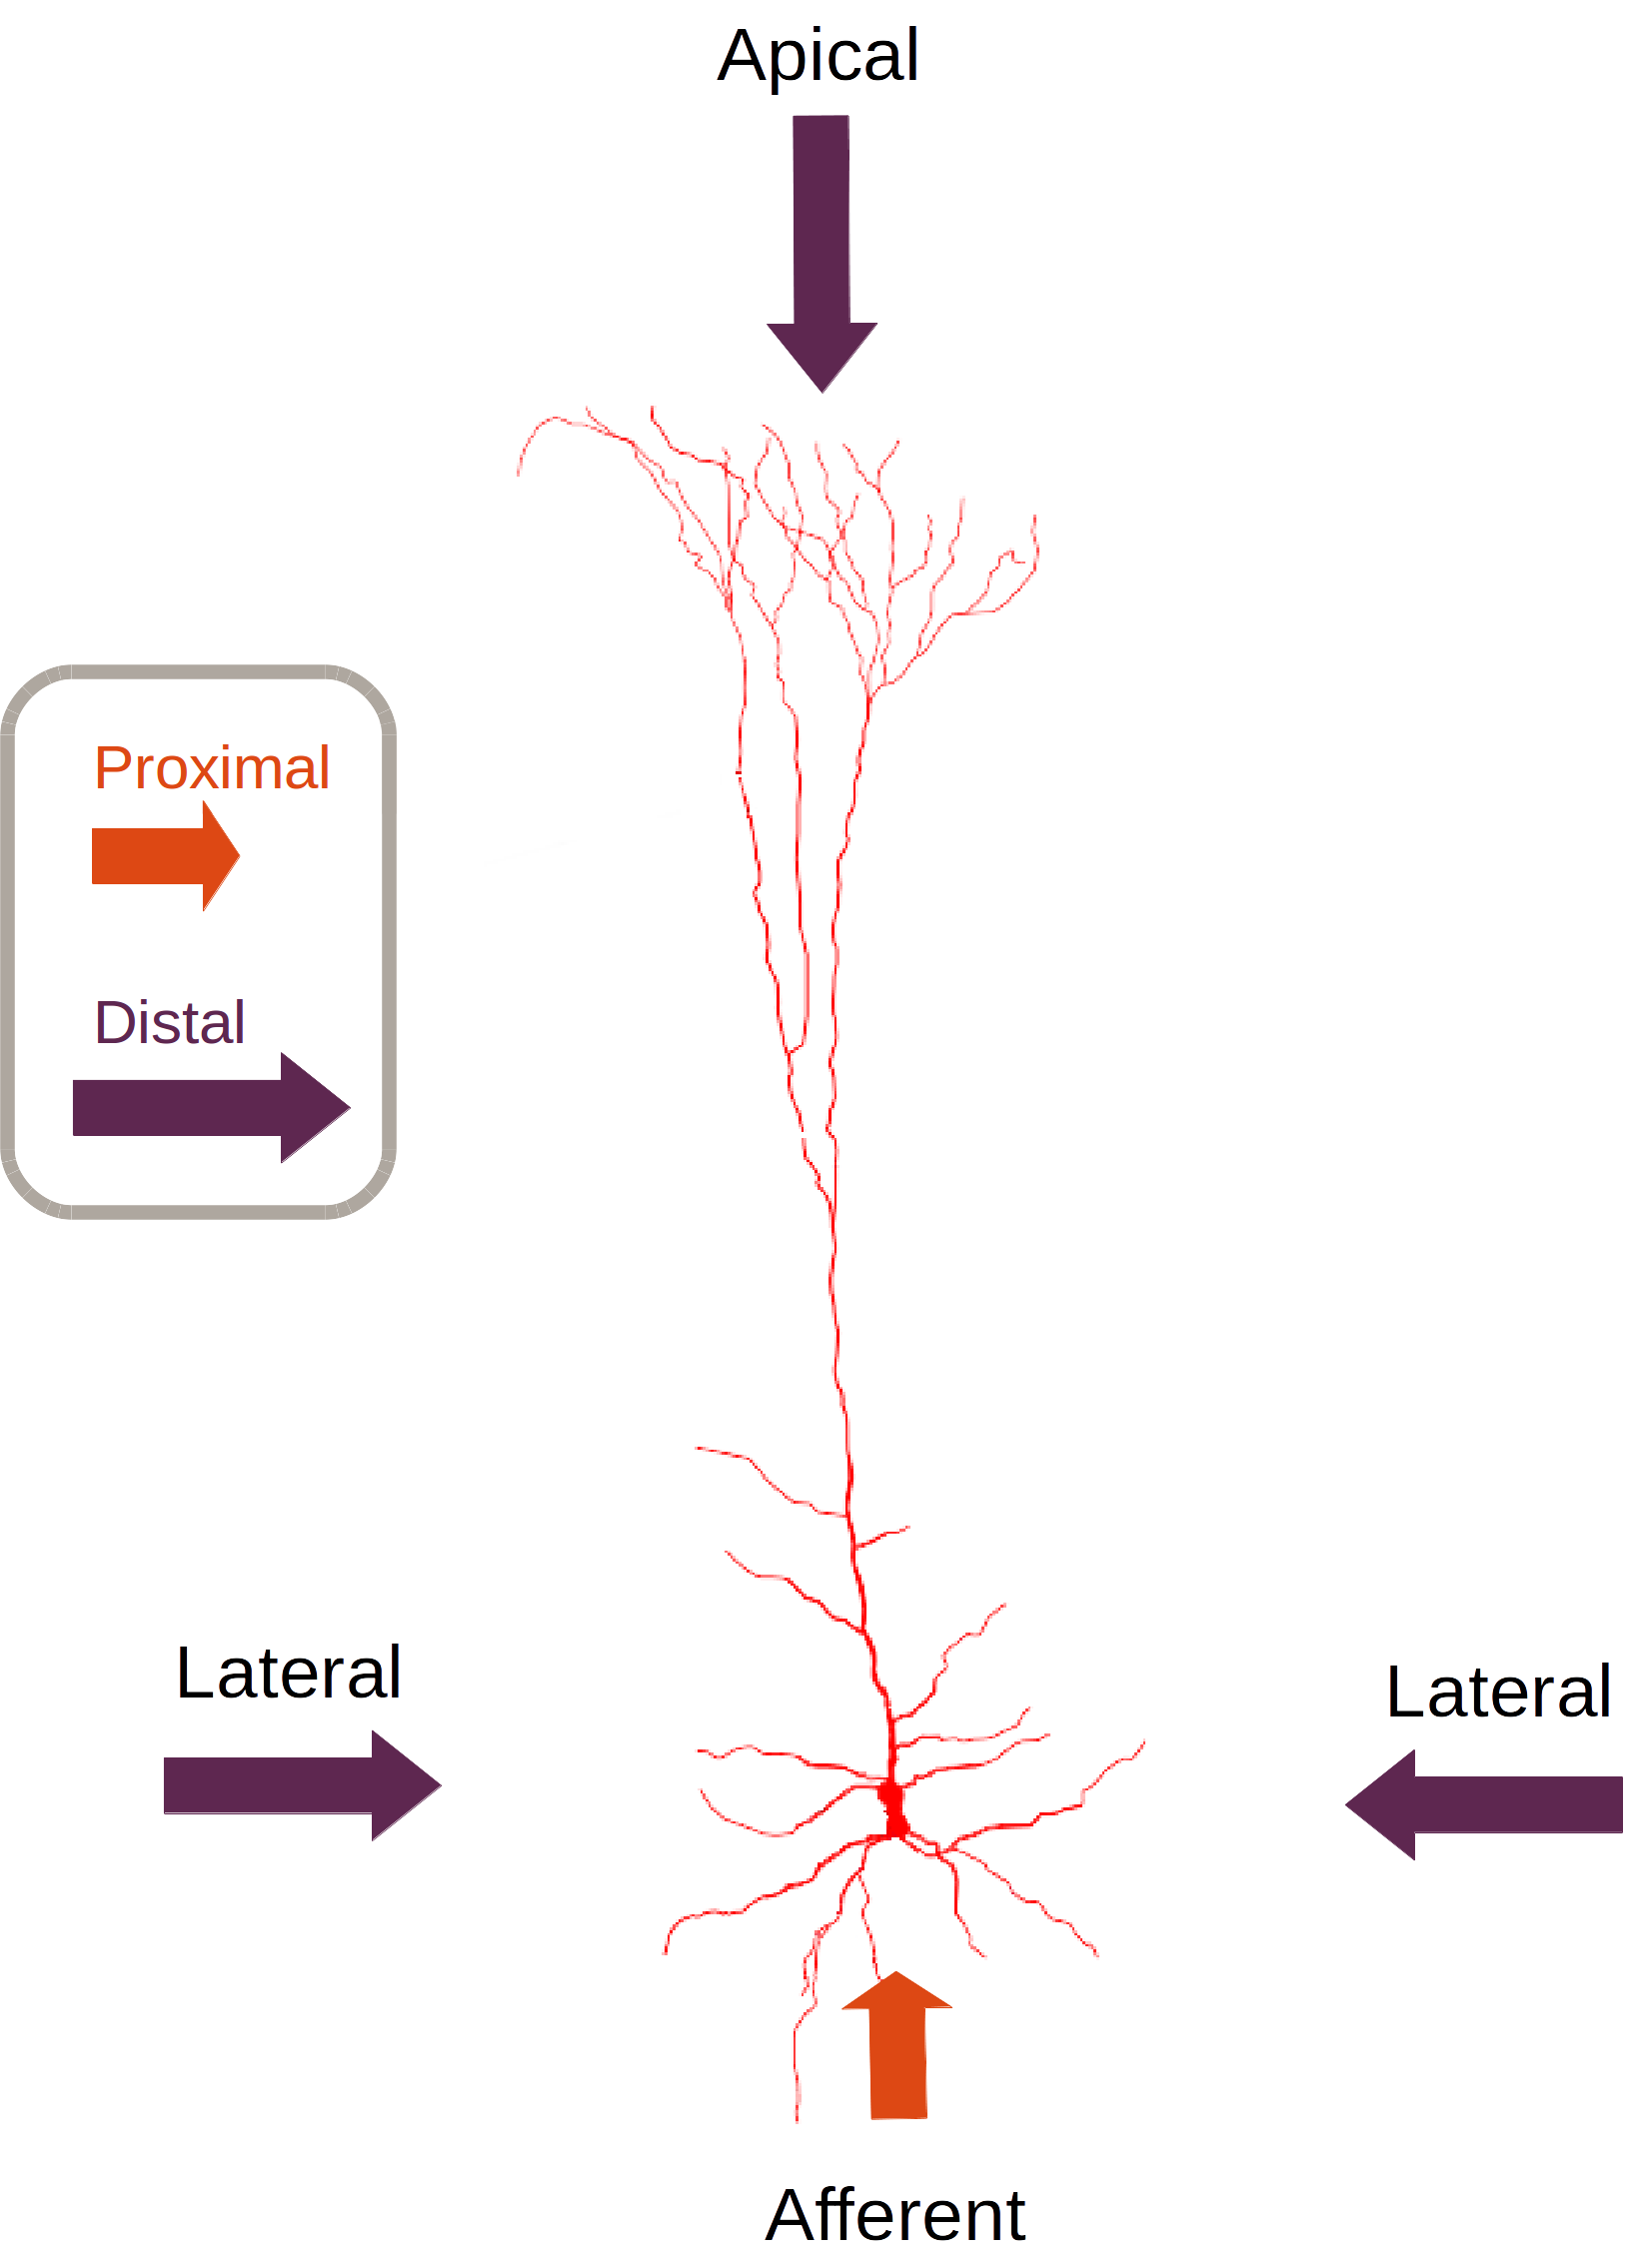
\includegraphics[width=0.5\textwidth]{Pyramidal_Cell.png}
    \caption{Perfil de conectividad de una unidad neuronal piramidal en la \gls{el}. Adaptado de (Fabuio - Own work, CC BY 4.0, \protect\url{https://commons.wikimedia.org/w/index.php?curid=60707501)}}
    \label{fig:Pyramidal_Cell}
\end{figure}

En la Fig.~\ref{fig:EncoderColumnConnections1} las conexiones próximas están solo compuestas por conexiones aferentes desde el algoritmo \gls{mrstsa} mientras que las conexiones distales están compuestas por conexiones laterales y apicales desde columnas vecinas y desde columnas en otra capa foránea respectivamente.
La información aferente activa diferentes clusters de unidades en una \gls{cc} estableciendo una primera aproximación de los rasgos fonéticos abstraídos desde el flujo auditivo de entrada. 
La \gls{el} refina tales rasgos crudos por medio de activaciones contextuales previas producidas en la misma \gls{cc} y/o en \gls{cc_pl} vecinas.
Tal información contextual es enviada a cada \gls{cc} por medio de ramas dendríticas distales laterales que trabajan como elementos de procesamiento independientes en una célula (Fig.~\ref{fig:Lateral_Distal_Connections}).
La activación actual en tales elementos dendríticos afectarán la manera en la que las células reciben información aferente futura.

\begin{figure*}[tb] 
    \centering
    \subfloat[Ramas dendríticas distales laterales en un campo receptivo en la \gls{el}.\label{sub:Distal_Lateral_Dendrites}]{%
       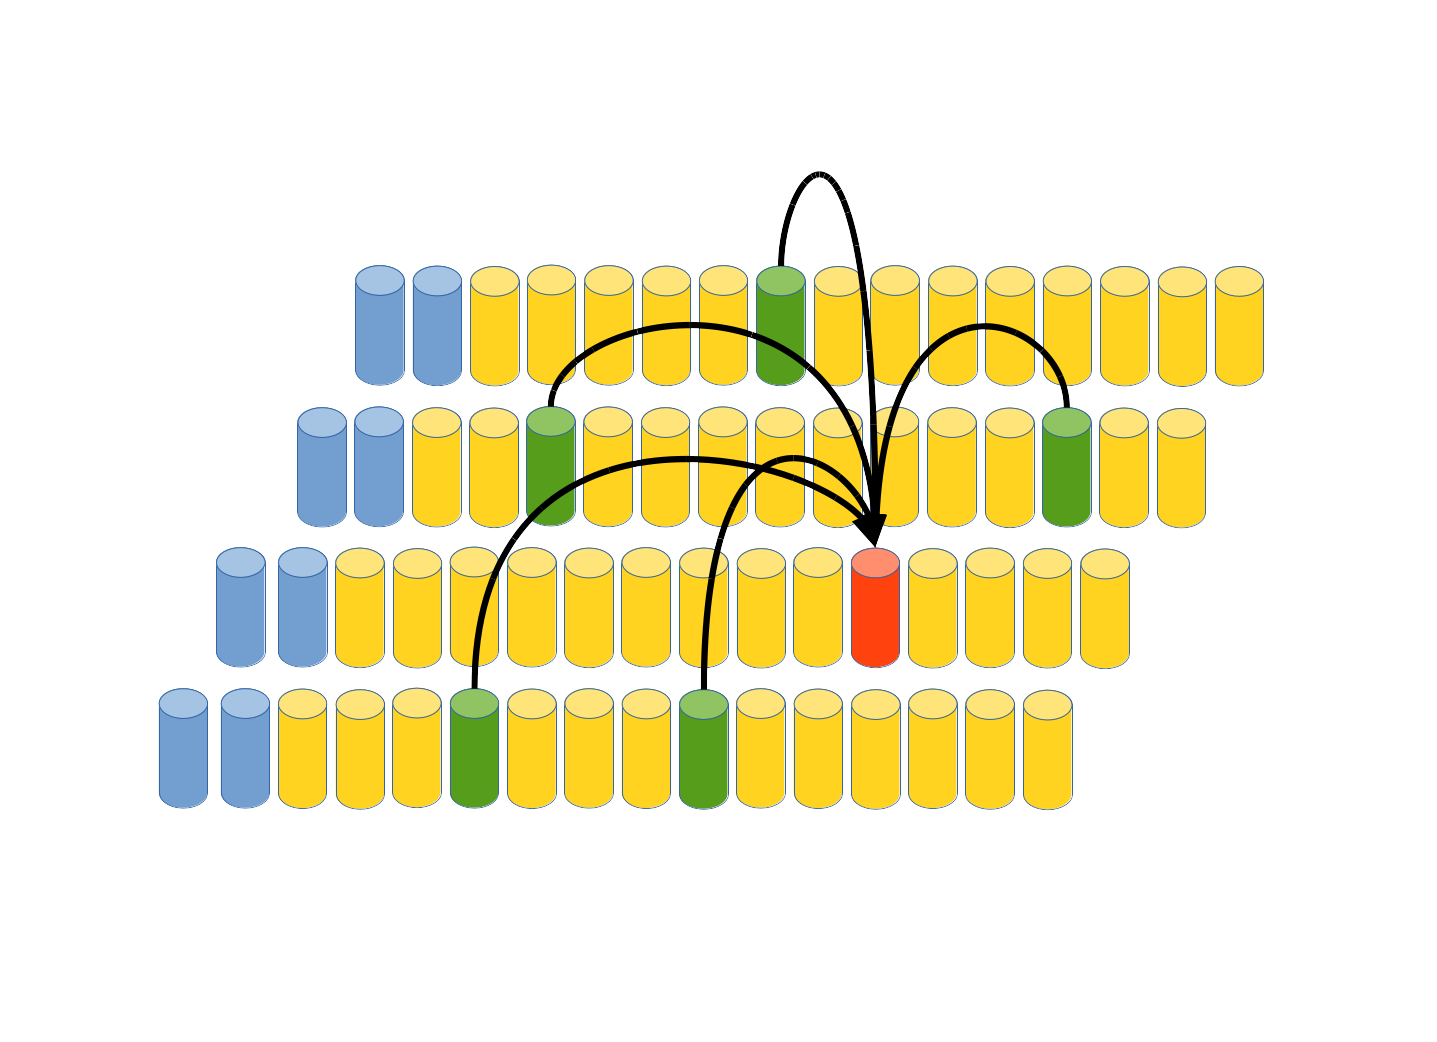
\includegraphics[width=0.482\linewidth]{Distal_Lateral_Dendrites.png}}
    \hfill
  \subfloat[Sinapsis potenciales en una rama dendrítica distante.\label{sub:Distal_Lateral_Potential_Connections}]{%
	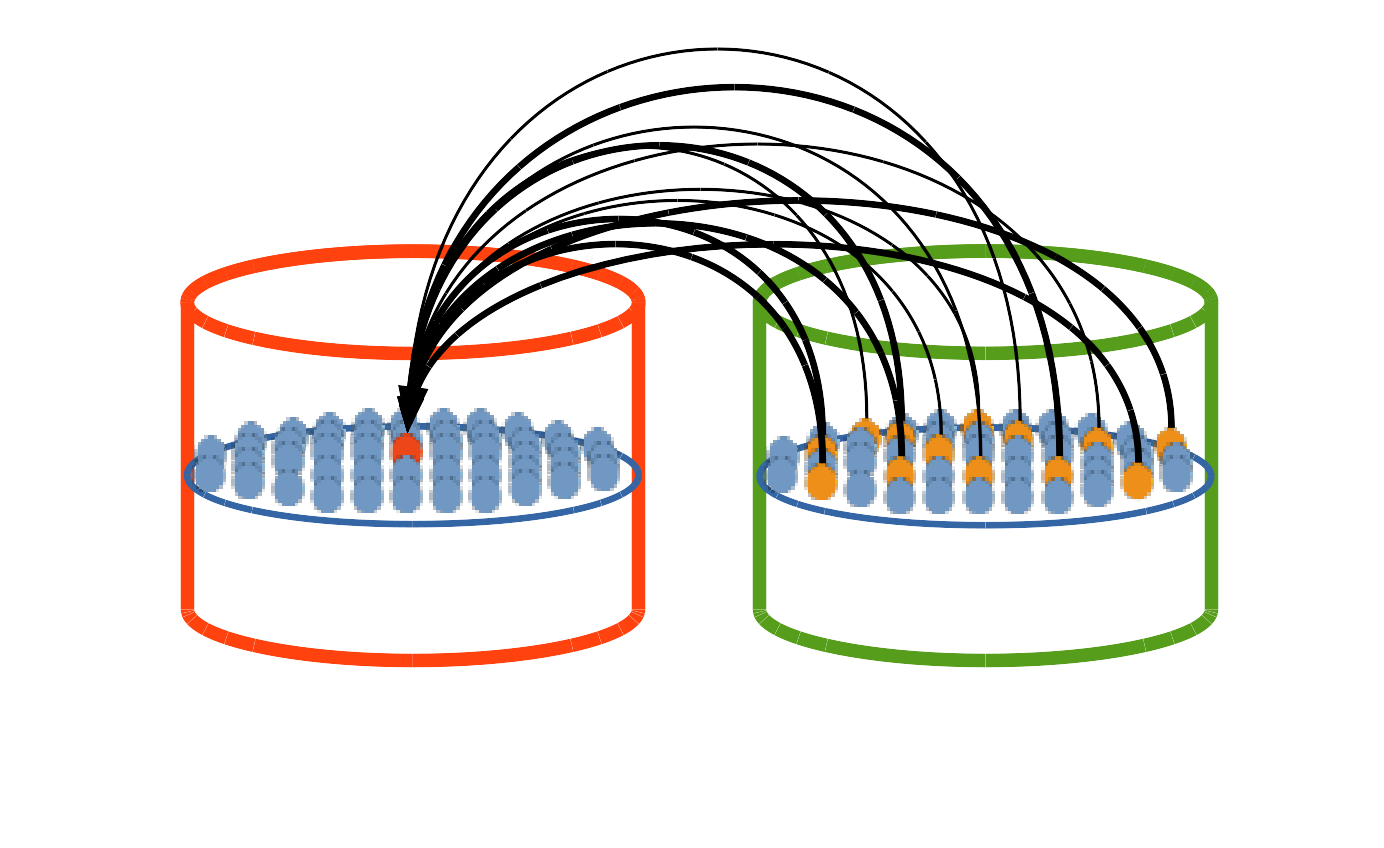
\includegraphics[width=0.482\linewidth]{Distal_Lateral_Potential_Connections.png}}
\\
  \subfloat[Contraparte biológica para las sinapsis potenciales en una rama dendrítica distal.\label{sub:Biological_Dendrite}]{%
       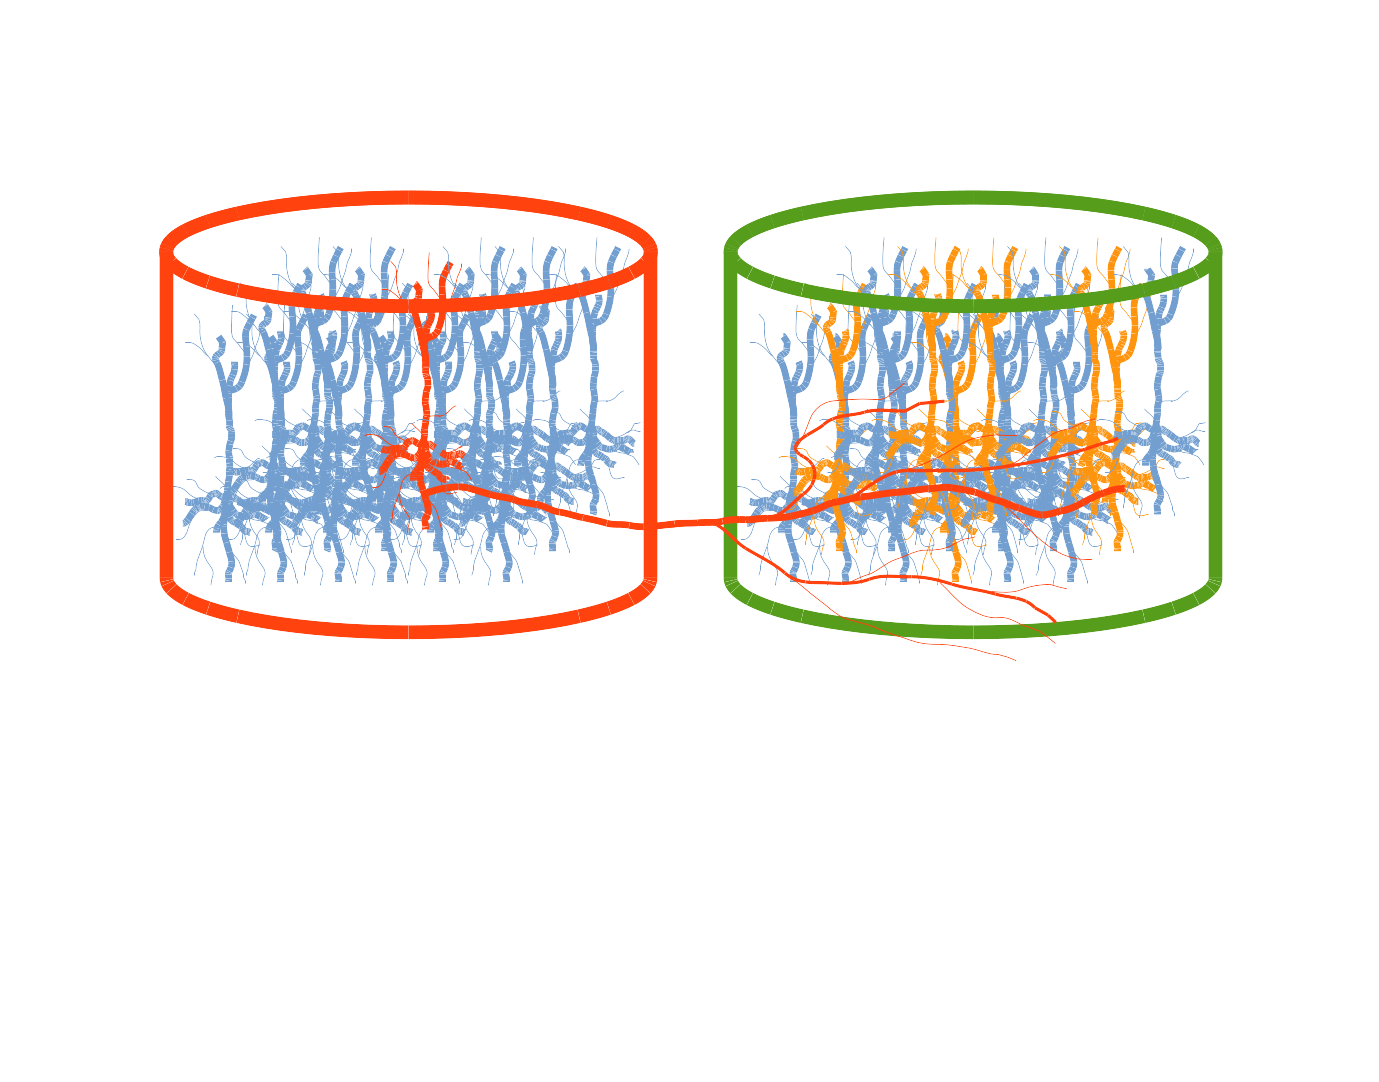
\includegraphics[width=0.482\linewidth]{Biological_Dendrite.png}}
    \hfill
    \subfloat[Crecimiento snaptico biológico en dendritas distales.\label{sub:Biological_Synapse}]{%
	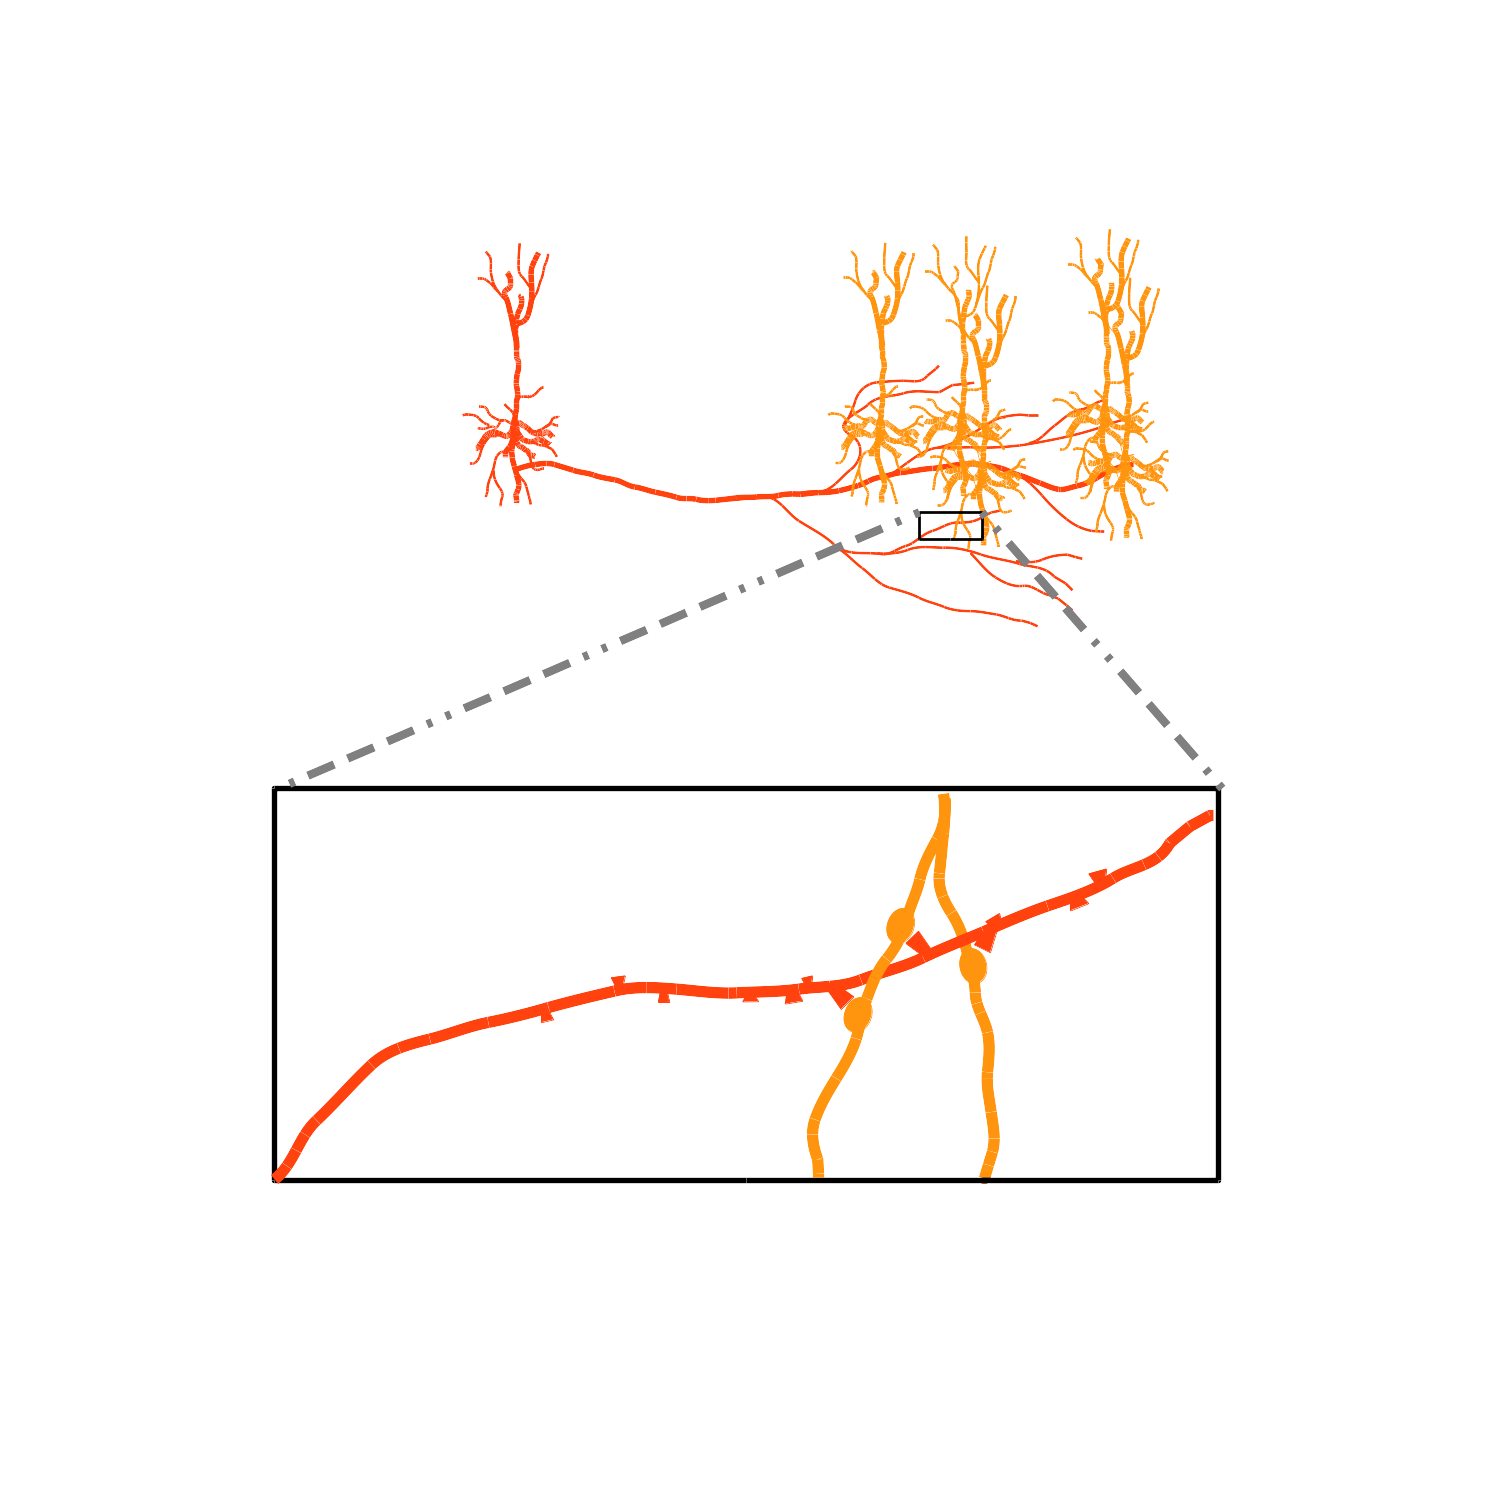
\includegraphics[width=0.482\linewidth]{Biological_Synapse.png}}
	\caption{Conectividad dendrítica distal en la \gls{el}.}
  \label{fig:Lateral_Distal_Connections} 
\end{figure*}

Las conexiones dendríticas distales se muestran en la Fig.~\ref{fig:Lateral_Distal_Connections}.
En la Fig.~\ref{sub:Distal_Lateral_Dendrites} las ramas dendríticas distales convergen desde \gls{cc_pl} vecinas dentro del campo receptivo de una \gls{cc} en la \gls{el}.
Una rama dendrítica distante entre la \gls{cc} roja y una \gls{cc} verde implica que cada unidad neuronal en la \gls{cc} roja está vinculada con un conjunto diferente de unidades neuronales en la \gls{cc} verde por medio de conexiones potenciales.
En la Fig.~\ref{sub:Distal_Lateral_Potential_Connections} tales conexiones potenciales en una rama dendrítica vinculan una unidad neuronal en la \gls{cc} roja con un subconjunto de unidades neuronales en una \gls{cc} verde.
El subconjunto de conexiones potenciales constituye un porcentaje de unidades neuronales dentro de la \gls{cc} verde.
Tal porcentaje es un parámetro ajustable para la \gls{cc}.
La Fig.~\ref{sub:Biological_Dendrite} muestra una rama dendrítica distal biológica entre una célula piramidal en una \gls{cc} y un subconjunto de células piramidales en una \gls{cc} vecina dentro de su campo receptivo en la \gls{el}.
Esta es la contraparte biológica de la Fig.~\ref{sub:Distal_Lateral_Potential_Connections}.
La Fig.~\ref{sub:Biological_Synapse} muestra cómo la proximidad física de una rama dendrítica desde la célula roja a las ramas axonales desde las células amarillas constituyen conexiones potenciales que podrían prosperar convirtiéndose en sinapsis establecidas dependiendo de la actividad secuencial entre células.

En la Fig.~\ref{fig:Lateral_Distal_Connections} se puede ver que la dispersión y aleatoriedad en el perfil de conectividad de nuestro modelo computacional se manifiesta a diferentes escalas.
Tal fenómeno no solo se implementa a escala macro como se observa en la Fig.~\ref{sub:Distal_Lateral_Dendrites} sino que también a escala micro como se puede ver en la Fig.~\ref{sub:Distal_Lateral_Potential_Connections}.
De hecho, la complejidad de nuestra implementación deriva en diferentes algoritmos sinápticos para las dendritas próximas y distales.
Mientras que las dendritas próximas implementan un \gls{som} de conectividad desde información aferente, las dendritas distales resultan en un mecanismo sináptico mucho más preciso para conseguir \gls{sdr_pl} desde una estructura predictiva secuencial en la que ramas dendríticas individuales actúan como elementos computacionales activos e independientes.
}{
\section{Cortical Spectro-Temporal Model (CSTM)}

The \gls{cstm} introduced in this paper constitutes a set of algorithms for the simulation of early phonetic acquisition in cortical dynamics~\cite{10.1371/journal.pone.0217966}. Fig.~\ref{fig:EncoderColumnConnections1} shows a representation of the \gls{cstm} centered in a connection scheme for a cortical column in the \glsfirst{el}--the central algorithm in the~\gls{cstm}. Each cylinder in the \gls{el} and in the \glsfirst{cl} represents a \glsfirst{cc} in neural tissue. Each prism in the \glsfirst{mrstsa} represents a \gls{a1} activation, (implemented as a real valued variable in the~\gls{mrstsa}). The figure is a visualization of a \gls{cc} (in red) and its three receptive fields (in yellow). The receptive field of a \gls{cc}--on the \gls{el} or the \gls{cl}--is an array that defines a set of \glspl{cc} with which such column could be connected. The receptive field of a \gls{cc} on the \gls{mrstsa} determines an array of real valued variables with which such column could be connected. A subset of \glspl{cc} in a receptive field (in green) represents a sparse and random set of \glspl{cc} that are really connected with the \gls{cc} in red. A similar scenario could be described for the green prisms on the \gls{mrstsa}. The size, wrap-around property and percentage of established links (in green) inside a receptive field are tunable parameters for the \gls{el}. In this work, only lateral connections have been implemented. There is no apical dendritic branches in the \gls{el} since, in the current implementation, there are no upper \glspl{cl} from which to bring such connections. We have already implemented \glspl{cl} which can receive afferent inputs from the \gls{el} outputs, but we have not been able to test those algorithms properly yet. Regardless of it, we decided to include the \gls{cl} in Fig.~\ref{fig:EncoderColumnConnections1} in order to show that lateral connections from neighboring \glspl{cc} have the same algorithmic nature than apical connections from the \glspl{cl} above the \gls{el}.

In this way, Fig. \ref{fig:EncoderColumnConnections1} shows the data flow of the information converging to a \gls{cc} inside the \gls{el}. First of all, our Corpora Generation algorithm is used to produce audio files containing the uttered corpora generated by means of speech synthesis tools. The algorithm generates cross synthesizer standard mark up language files with SABLE \cite{sable} format. In such files, \gls{festival} synthesizer is instructed to generate corpora from several number of words from different vocabularies uttered by different voices available from the synthesizer. The organization of the corpora has certain rules and restrictions in order to avoid biases in the training processes. The voices are sequentially chosen (pseudo-randomly) with the restriction that no voice could utter a second time until all the voices had uttered in their turns. Every voice utters certain number of words per turn--in pseudo-random order--and no word is repeated until all the words are used by such voice. Every word in the audio file is followed by a silence gap whose time is equivalent to the uttering time of certain monosyllabic word. We use the \texttt{text2wave} program provided by Festival in order to generate a \texttt{wav} file from the SABLE file.

Second, sound waves from the audio files are processed by the \gls{mrstsa} algorithm. In this paper we show an implementation that prompts the parsimonious incorporation of neurophysiological properties--mainly centered in cortical features. In such sense, we followed the main guidelines in the implementation of the cortical section of Chi T. et al. \cite{chi_2005} model in order to implement the \gls{mrstsa} algorithm. We implemented the initial stage in the \gls{mrstsa} with the application of \gls{fft} to the audio vector with a different sample window for each resolution. We then extracted the power spectral density from each resolution. In this way we obtained a multiresolution spectral analysis of the audio signal, with high spectral and low temporal resolution for wider sample windows and vice versa. Such different time windows in the \gls{fft}, incorporated--at the same time--leakage low-pass filters with a time constant for each resolution accounting for decrease of phase-locking in the auditory nerve~\cite{chi_2005}. We then applied a \gls{mfb} with 128 elements to each spectrum in order to represent the spectral analysis performed by the cochlear filter bank. Then, we convolved each resolution obtained in the last step along its tonotopic axis with a complex multiresolution function whose real part was a symmetric Mexican hat function and its imaginary part was its antisymmetric Hilbert transform. With this strategy we incorporated additional neuro-physiological phenomena such as symmetry \cite{shamma_1993}, bandwidth \cite{schreiner_1990} and frequency modulation selectivity \cite{shamma_1993,heil_1992,mendelson_1985} found in \gls{a1} and incorporated in the original algorithms \cite{wang_1995}.

Finally, the \gls{el} simulates a patch of cortical tissue using an n-dimensional array of complex structures called \glspl{csom} that simulate \glspl{cc} in the brain. The \gls{el} generates \glspl{sdr} \cite{ahmad_2016} from the inputs delivered by the \gls{mrstsa} stage and from the activation history in its own \glspl{cc}. \glspl{sdr} exhibit interesting mathematical properties which give them high noise rejection and fault tolerance \cite{DBLP:journals/corr/AhmadH15}. These are typical characteristics in cortical tissue where individual cells are far from 100\% reliable and the cells die and regenerate continuously. This algorithm incorporates neurophysiological phenomena such as columnar organization, afferent spontaneous micro-columnar formation, proximal and distal dendritic arborization, lateral intercolumn interaction by means of independent dendritic \gls{nmda} branch activations, \glspl{mfe} with contextual stimulus adaptation, proximal lateral intracolumn inhibition, \gls{ltp}, \gls{ltd}, \gls{stdp} and distal synaptic homeostatic regulations.

Each cell unit in a \gls{cc} has two types of dendritic branches; proximal and distal. Proximal and distal dendritic branches lead to proximal and distal connections in a cell unit respectively~\cite{10.1371/journal.pone.0217966}. Neural units in the \gls{el} simulates pyramidal cells in cortical tissue in the brain (Fig \ref{fig:Pyramidal_Cell}). 

\begin{figure}[h!]
    \centering
    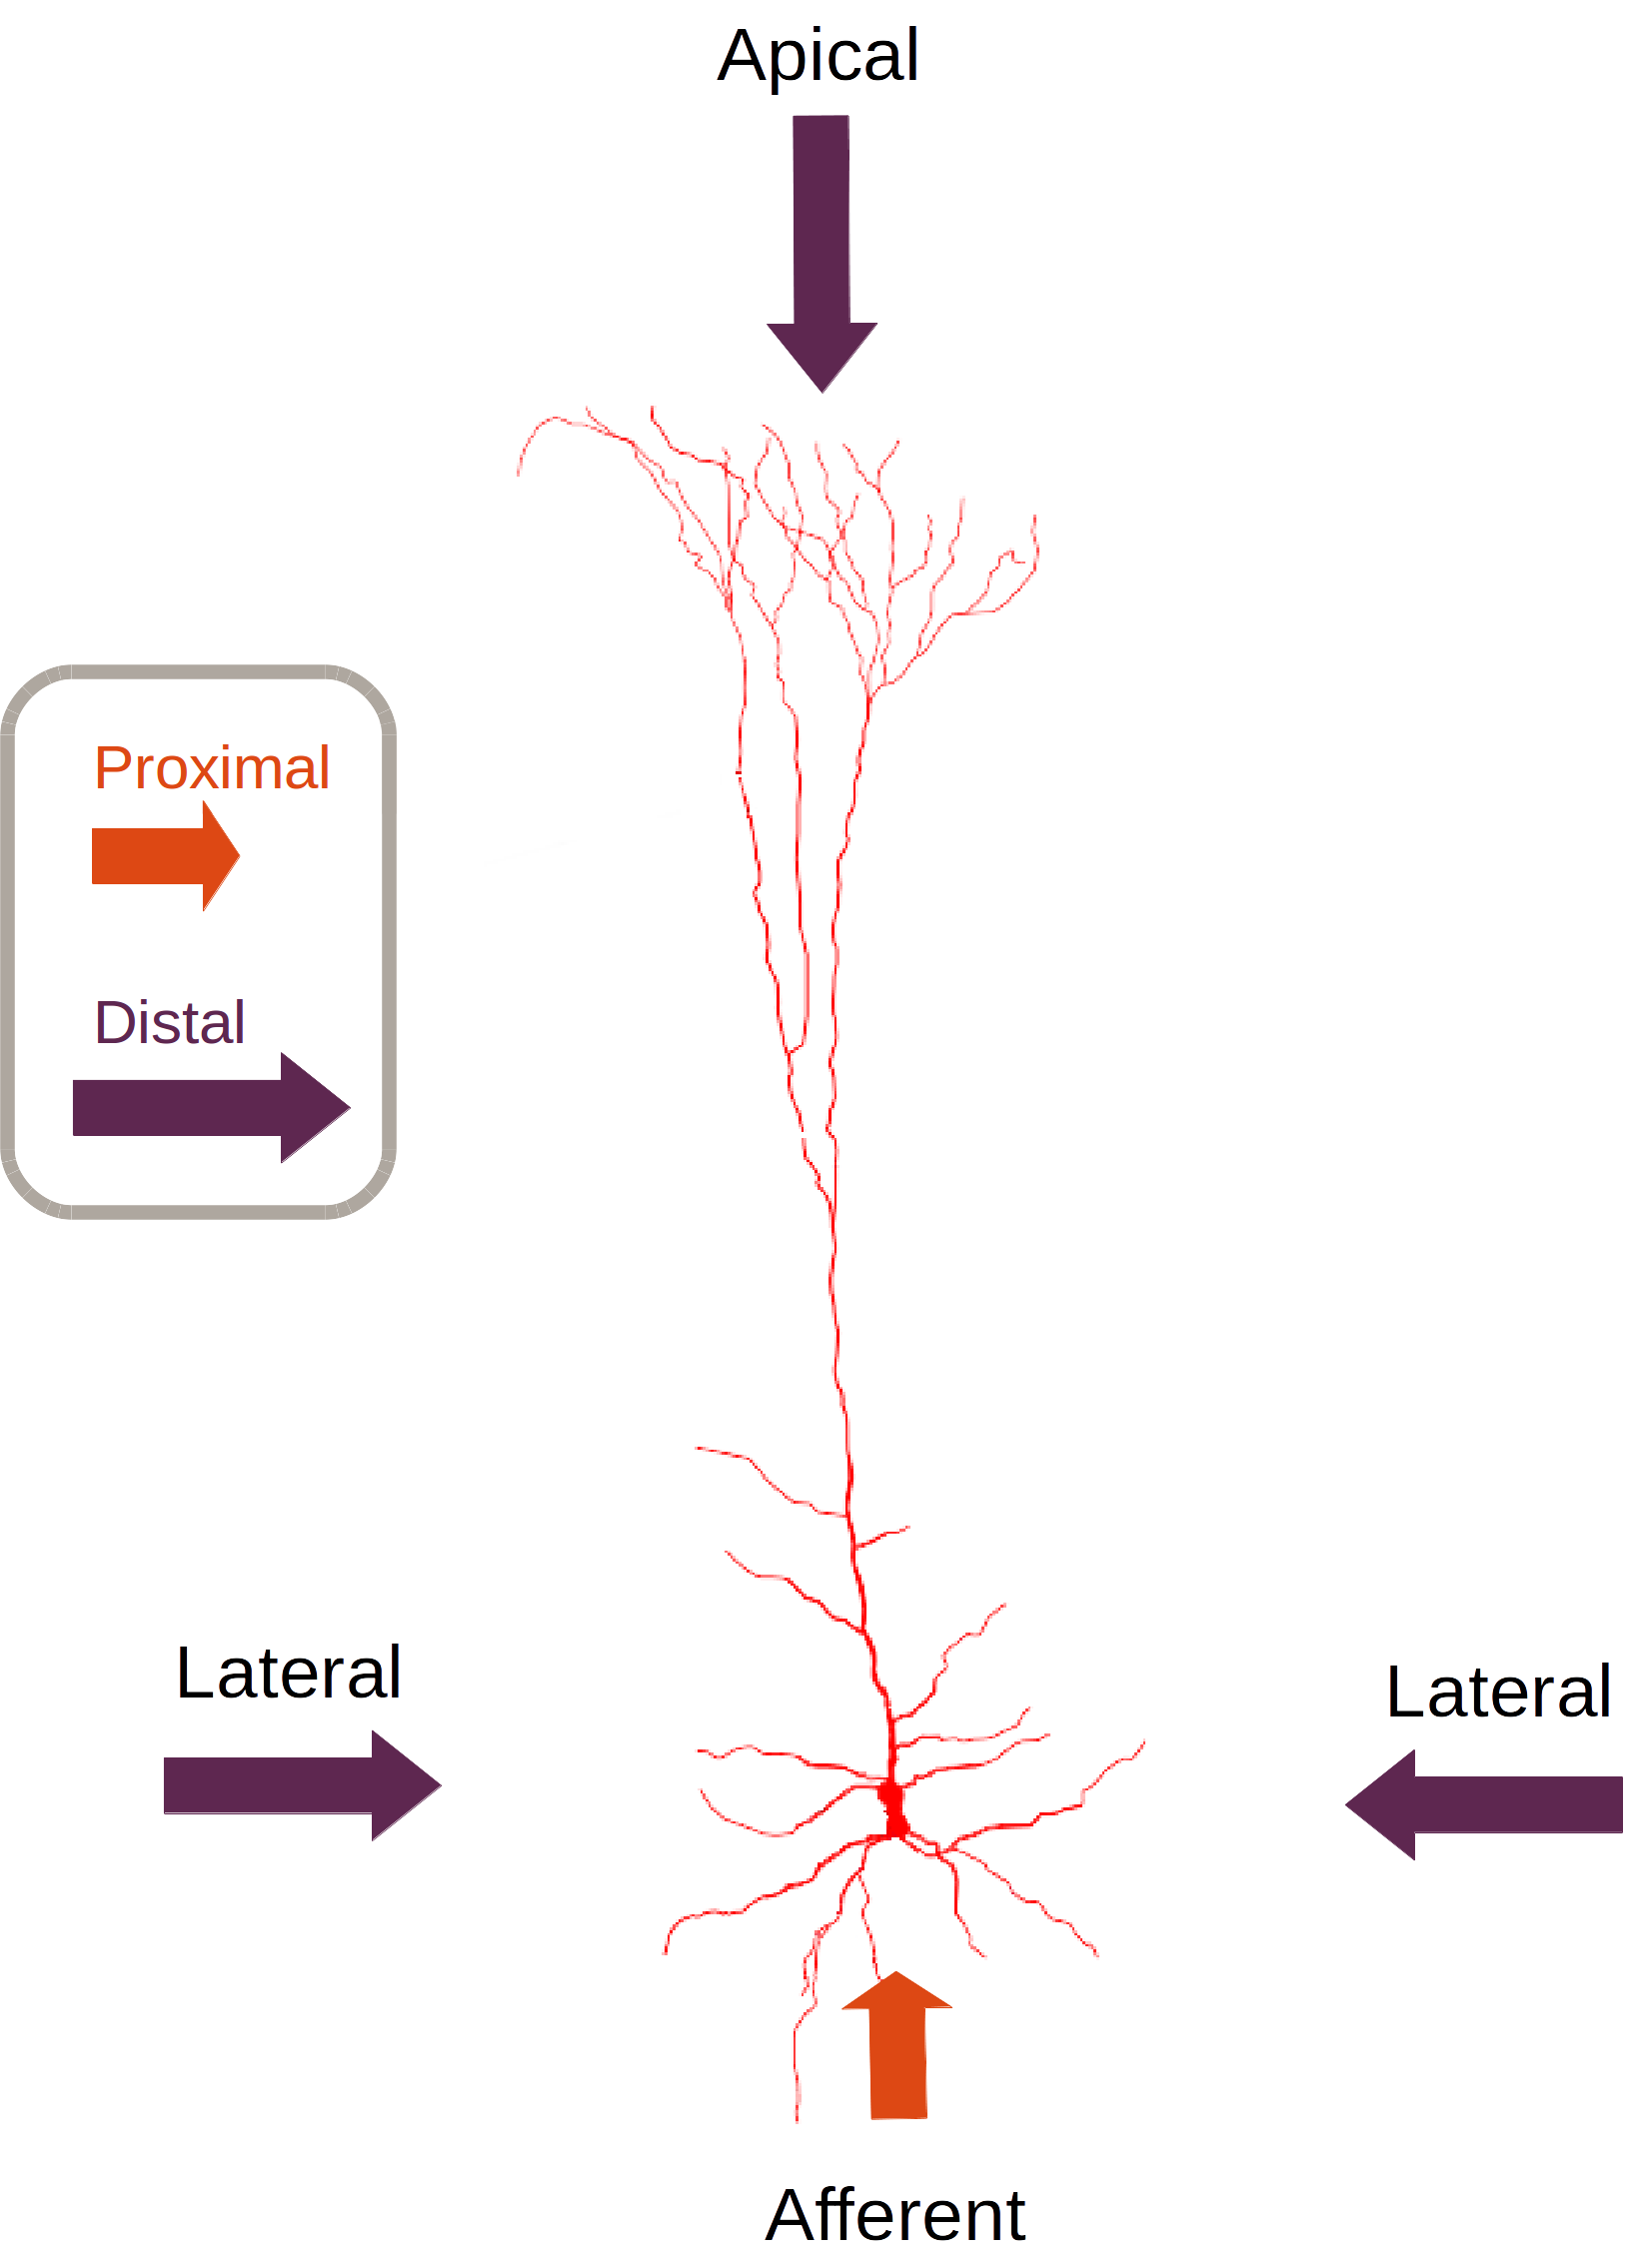
\includegraphics[width=0.3\textwidth]{Pyramidal_Cell.png}
    \caption{Connectivity profile of a pyramidal neural unit in the \gls{el}. Adapted from (Fabuio - Own work, CC BY 4.0, \protect\url{https://commons.wikimedia.org/w/index.php?curid=60707501)}}
    \label{fig:Pyramidal_Cell}
\end{figure}

In Fig.~\ref{fig:EncoderColumnConnections1} proximal connections are composed only by afferent connections from the \gls{mrstsa} algorithm while distal connections are composed by lateral and apical connections from neighboring columns and from columns in another cortical layer above respectively. Afferent information activates different clusters of units in a \gls{cc} establishing a first and raw approximation of the phonetic features abstracted from the input auditory stream. The \gls{el} fine-tunes such raw features by means of previous contextual activations produced in the same and/or in neighboring \glspl{cc}. Such contextual information is sent to each \gls{cc} by means of lateral distal dendritic branches which work as independent processing elements in a cell (Fig.~\ref{fig:Lateral_Distal_Connections}). Current activation in such dendritic elements will affect the way in which cells receives future afferent information.

\begin{figure*}[tb] 
    \centering
    \subfloat[Lateral distal dendritic branches in a receptive field in the \gls{el}.\label{sub:Distal_Lateral_Dendrites}]{%
       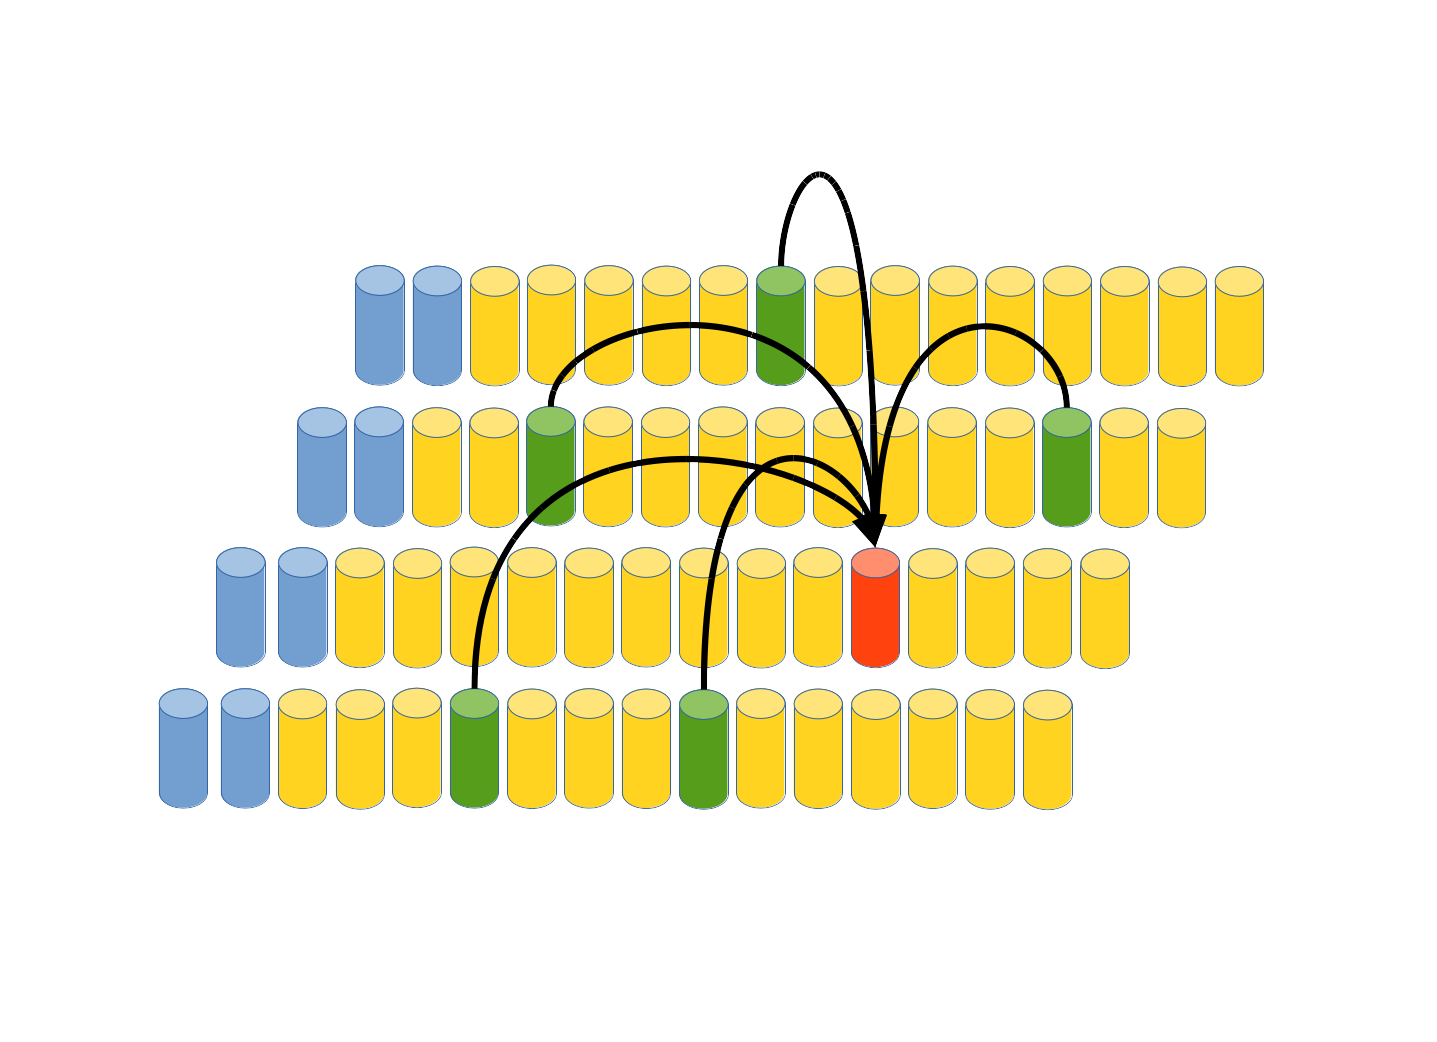
\includegraphics[width=0.482\linewidth]{Distal_Lateral_Dendrites.png}}
    \hfill
  \subfloat[Potential synapses in a distal dendritic branch.\label{sub:Distal_Lateral_Potential_Connections}]{%
        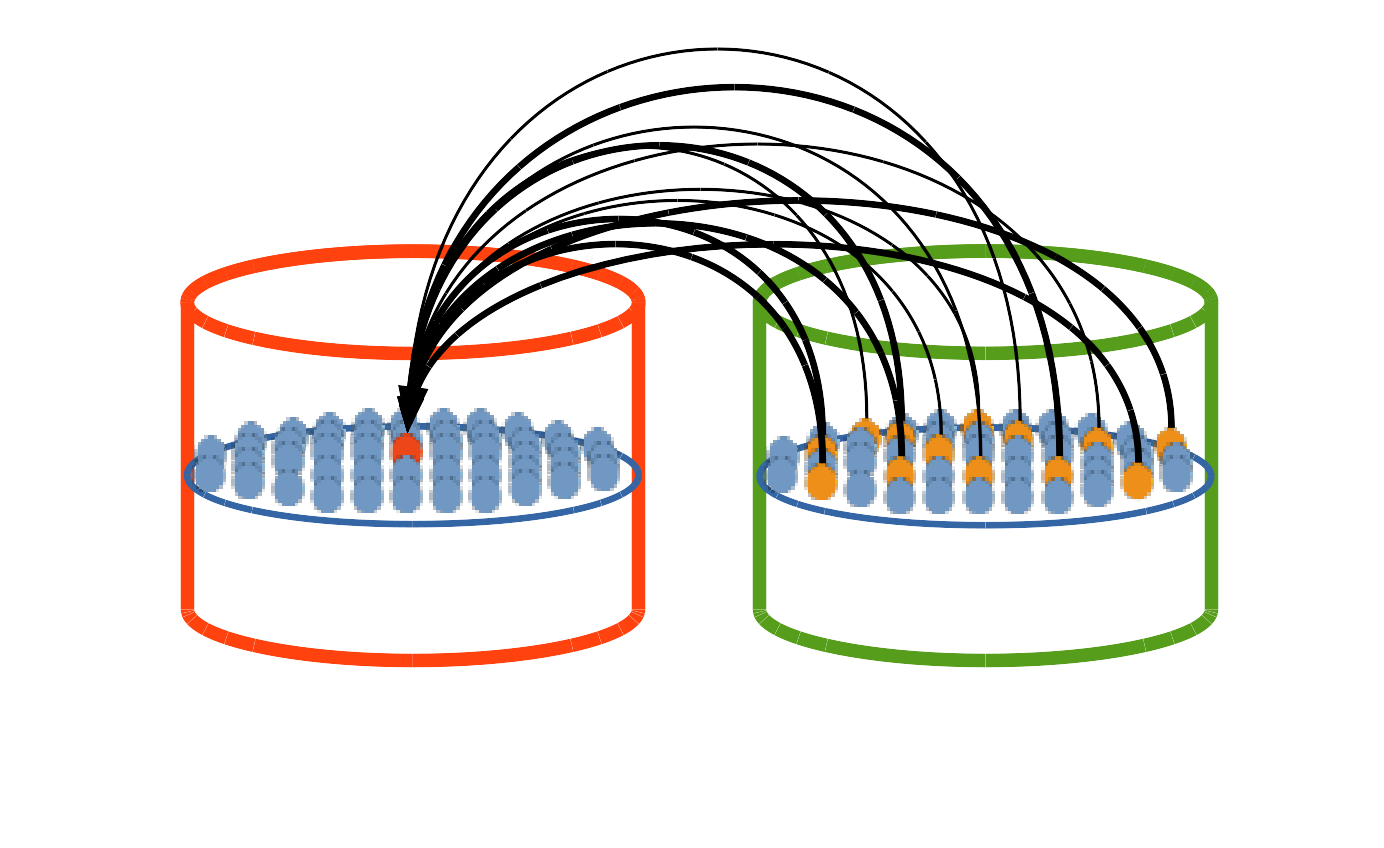
\includegraphics[width=0.482\linewidth]{Distal_Lateral_Potential_Connections.png}}
\\
  \subfloat[Biological counterpart for the potential synapses in a distal dendritic branch.\label{sub:Biological_Dendrite}]{%
       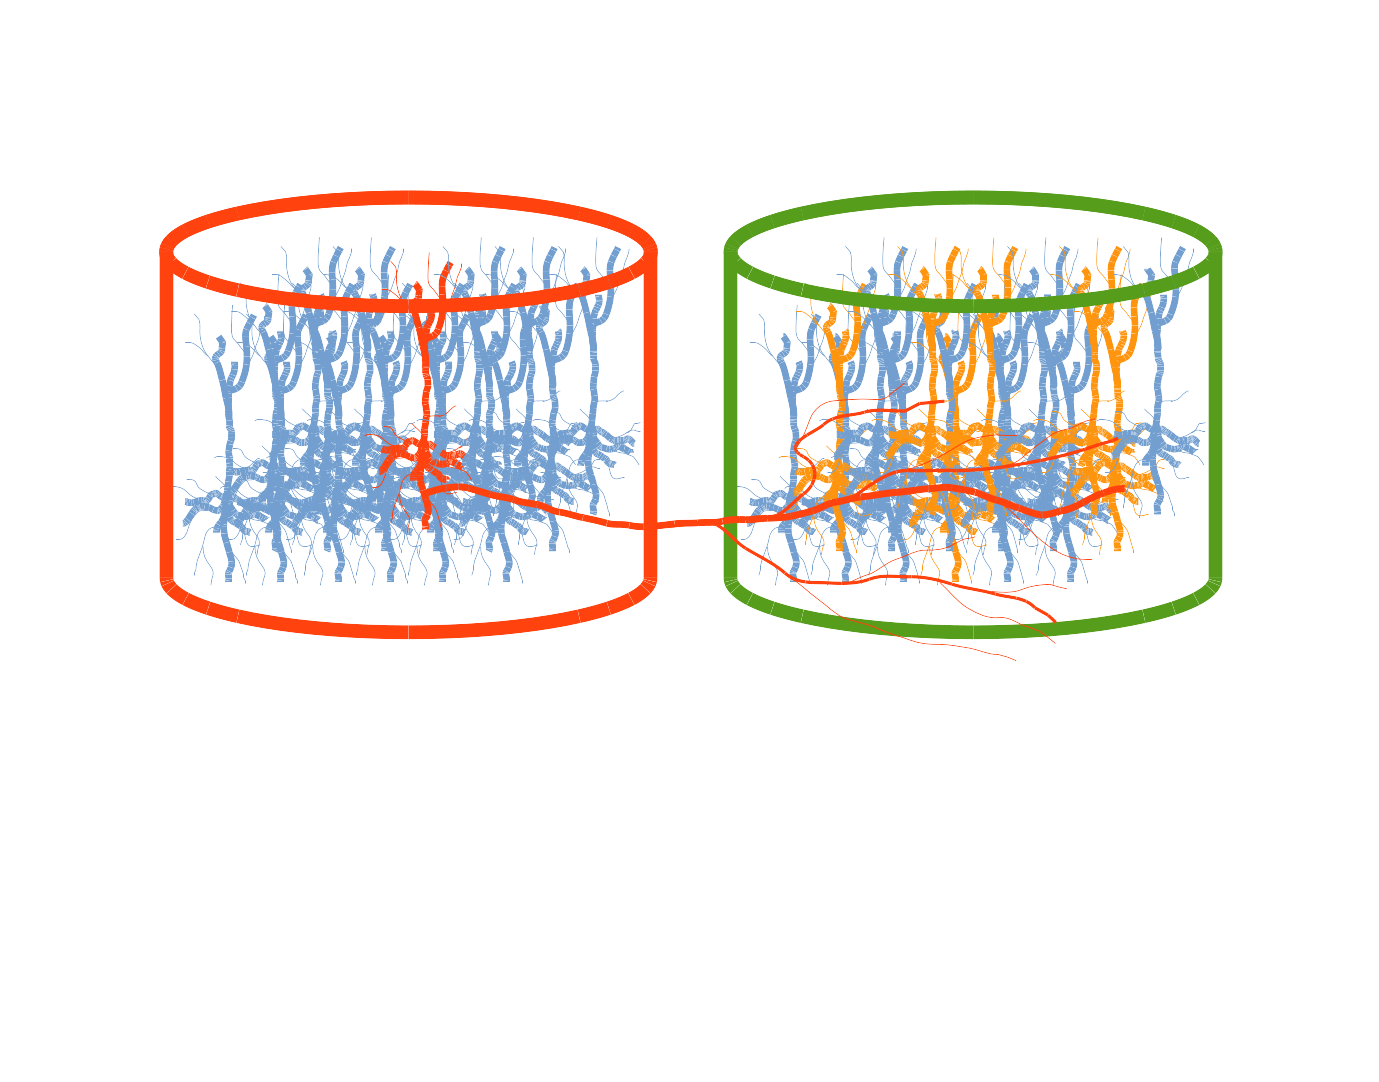
\includegraphics[width=0.482\linewidth]{Biological_Dendrite.png}}
    \hfill
    \subfloat[Biological synaptic grow in distal dendrites.\label{sub:Biological_Synapse}]{%
        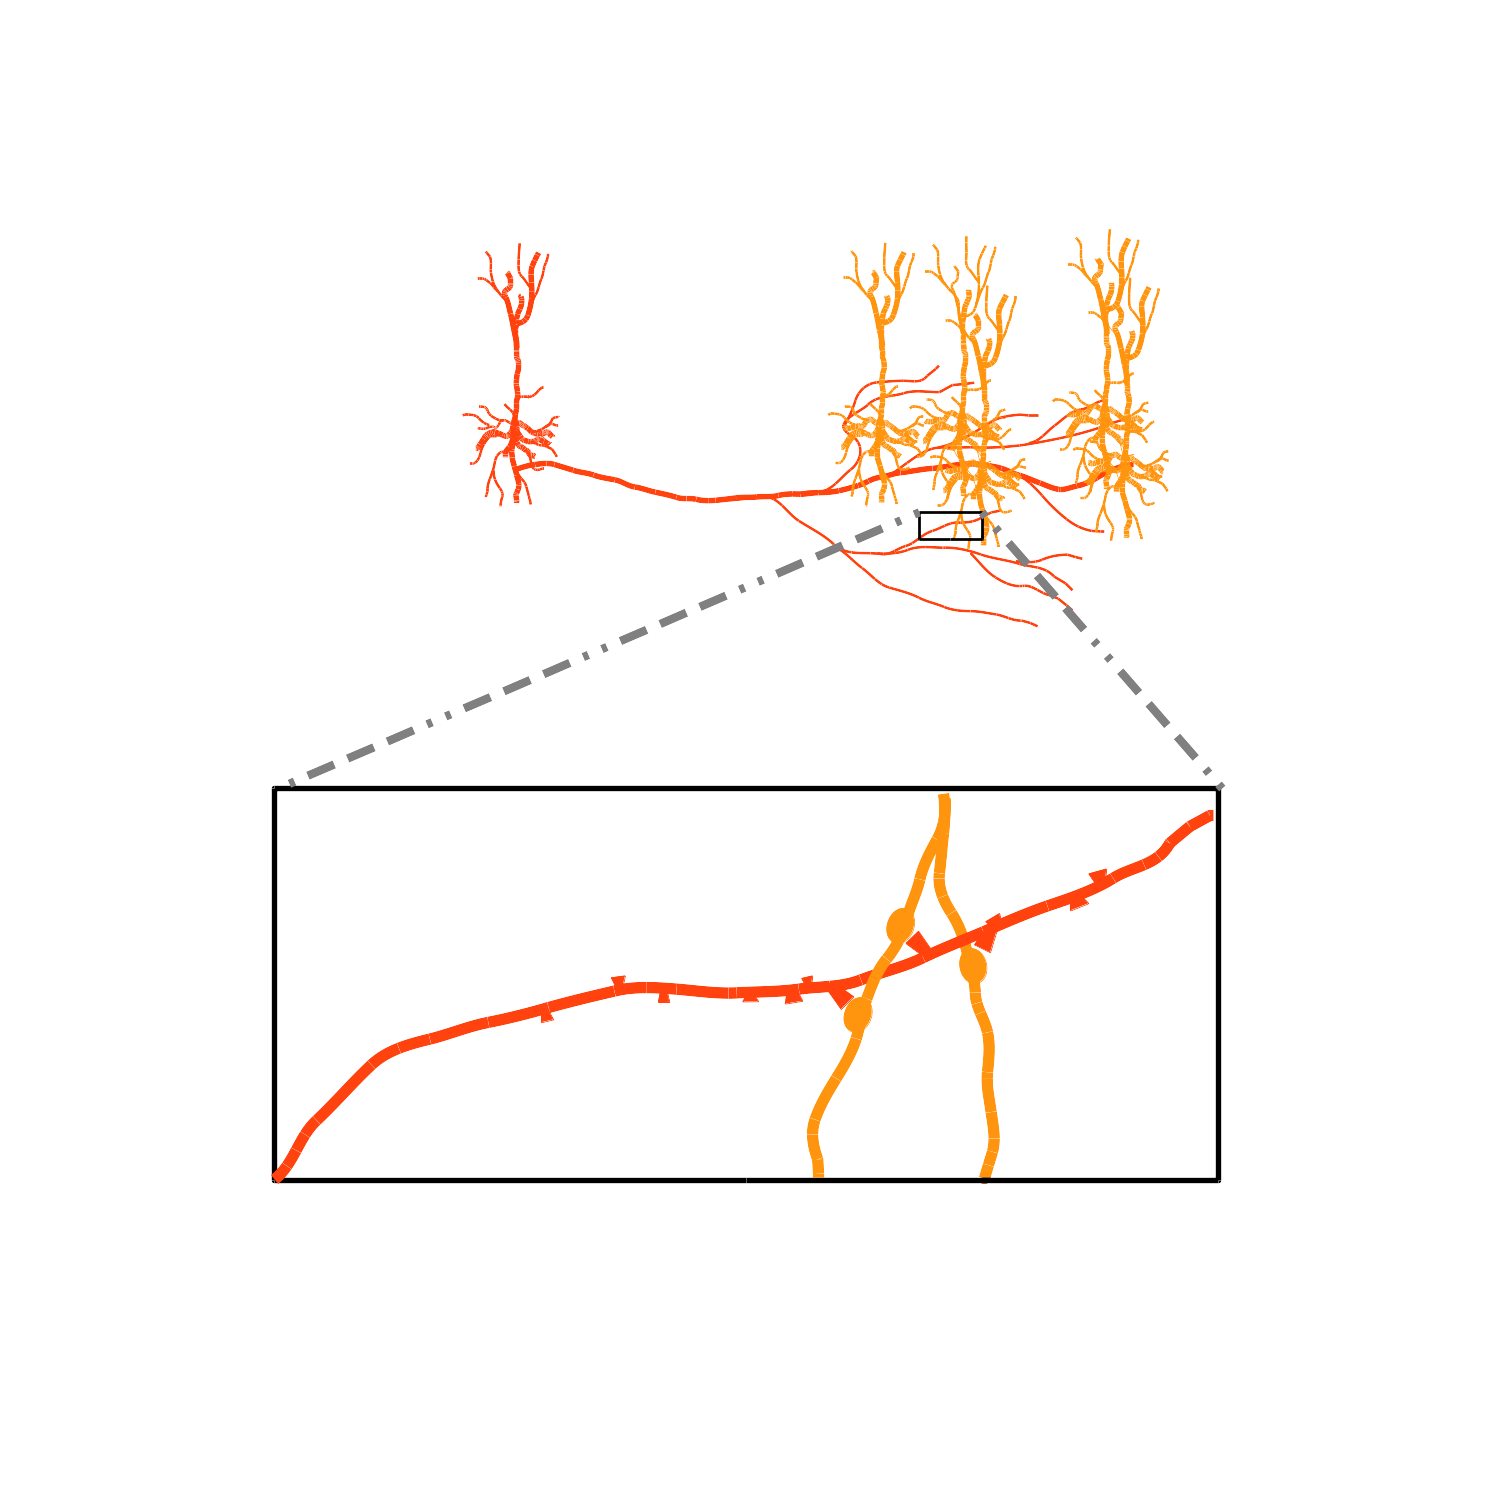
\includegraphics[width=0.482\linewidth]{Biological_Synapse.png}}
	\caption{Distal dendritic connectivity in the \gls{el}.}
  \label{fig:Lateral_Distal_Connections} 
\end{figure*}

Distal dendrite connections are shown in Fig.~\ref{fig:Lateral_Distal_Connections}. In Fig.~\ref{sub:Distal_Lateral_Dendrites} distal dendritic branches converge from neighboring \glspl{cc} inside the receptive field of a \gls{cc} in the \gls{el}. A distal dendritic branch between the red \gls{cc} and a green \gls{cc} implies that every neural unit in the red \gls{cc} is linked with a different subset of neural units in the green \gls{cc} by means of potential connections. In Fig.~\ref{sub:Distal_Lateral_Potential_Connections} such potential connections in a dendritic branch link a neural unit in the red \gls{cc} with a subset of neural units in a green \gls{cc}. The subset of potential connections constitutes a percentage of neural units inside the green \gls{cc}. Such percentage is a tunable parameter for the \gls{cc}. Fig.~\ref{sub:Biological_Dendrite} shows a biological distal dendritic branch between a pyramidal cell in a \gls{cc} and a sub-set of pyramidal cells in a neighboring \gls{cc} inside its receptive field in the \gls{el}. This is the biological counterpart of Fig.~\ref{sub:Distal_Lateral_Potential_Connections}. Fig.~\ref{sub:Biological_Synapse} shows how the physical proximity of a dendritic branch from the red cell to axonal branches from yellow cells constitutes potential connections which could prosper becoming in established synapses depending on the sequential activity among cells.

From Fig.~\ref{fig:Lateral_Distal_Connections} it can be seen that the sparseness and randomness in the connectivity profile of our computational model manifest at different scales. Such phenomena have not only a macro imprint as can be seen in Fig.~\ref{sub:Distal_Lateral_Dendrites} but also a micro imprint as can be seen in Fig.~\ref{sub:Distal_Lateral_Potential_Connections}. Furthermore, the complexity of our implementation derives in different synaptic algorithms for proximal and distal dendrites. While proximal dendrites implements a \gls{som} connectivity from afferent information, distal dendrites results in a much more precise synaptic mechanism to get~\glspl{sdr} from a sequential predictive structure in which individual dendritic branches act as independent and active computing elements.
}






















\iftoggle{DEBUG}{
\subsection{Implementación Paralela de la Generación de Corpus}
\label{CorpGenImp}

En cuanto a la producción paralela de los datos de entrada, generamos corpus con palabras mono y multi-silábicas escogidas aleatoriamente del idioma Inglés~\cite{10.1371/journal.pone.0217966} utilizando la síntesis de \emph{\gls{festival}} \cite{festival2014}.
A tales fines, también generamos archivos de marcado estándar para sintetizadores en lenguaje SABLE \cite{sable}.
En esos archivos instruimos \emph{\gls{festival}} a que genere archivos \texttt{wav} de audio con los corpus pronunciados por diferentes voces disponibles en el sintetizador.

Todo el código encargado de generar los corpus está implementado en Python y paralelizado por medio de un paquete \gls{mpi} para Python llamado \texttt{mpi4py}. 
La implementación algorítmica de esta paralelización se muestra en la Fig.~\ref{fig:CorporaGenerationParallelization}.
En tal figura, hay una distribución de generación de corpus entre procesos \gls{mpi} en Python.
Las tareas de generación de corpus se distribuyen entre procesos como un mazo de cartas se distribuye entre los jugadores de una partida.

En la Fig.~\ref{sub:Corpora_Generation_ALG} el esquema de paralelización distribuye vocabularios entre procesos \gls{mpi}.
En este algoritmo corremos un proceso \gls{mpi} por \gls{cpu}.
Cada proceso itera entre 0 y el número de vocabularios menos uno con un tamaño de paso de valor uno.
Pero, cada proceso desarrolla un vocabulario solo si el resto del número de iteración dividido por el número de procesos en el entorno \gls{mpi} es igual al identificador del proceso en cuestión.
De esta manera, teniendo 10 vocabularios y 3 procesos \gls{mpi}, el proceso número 0 desarrollará los vocabularios 0, 3, 6 y 9.
Todos los corpus que corresponden a cierto vocabulario son procesados de manera serial por el proceso que toma a cargo tal vocabulario.

La Fig.~\ref{sub:CorporaGenerationParallelization} muestra como cada proceso \gls{mpi} termina con un conjunto de vocabularios para generar los corpus correspondientes a tales vocabularios.
Si tenemos 10 corpus por vocabulario, el proceso 0 terminará generando 40 corpus serialmente, mientras que los procesos 1 y 2 generarán 30 corpus cada uno serialmente.

\begin{figure*}[tb] 
    \centering
  \subfloat[Algoritmo de paralelización.\label{sub:Corpora_Generation_ALG}]{%
       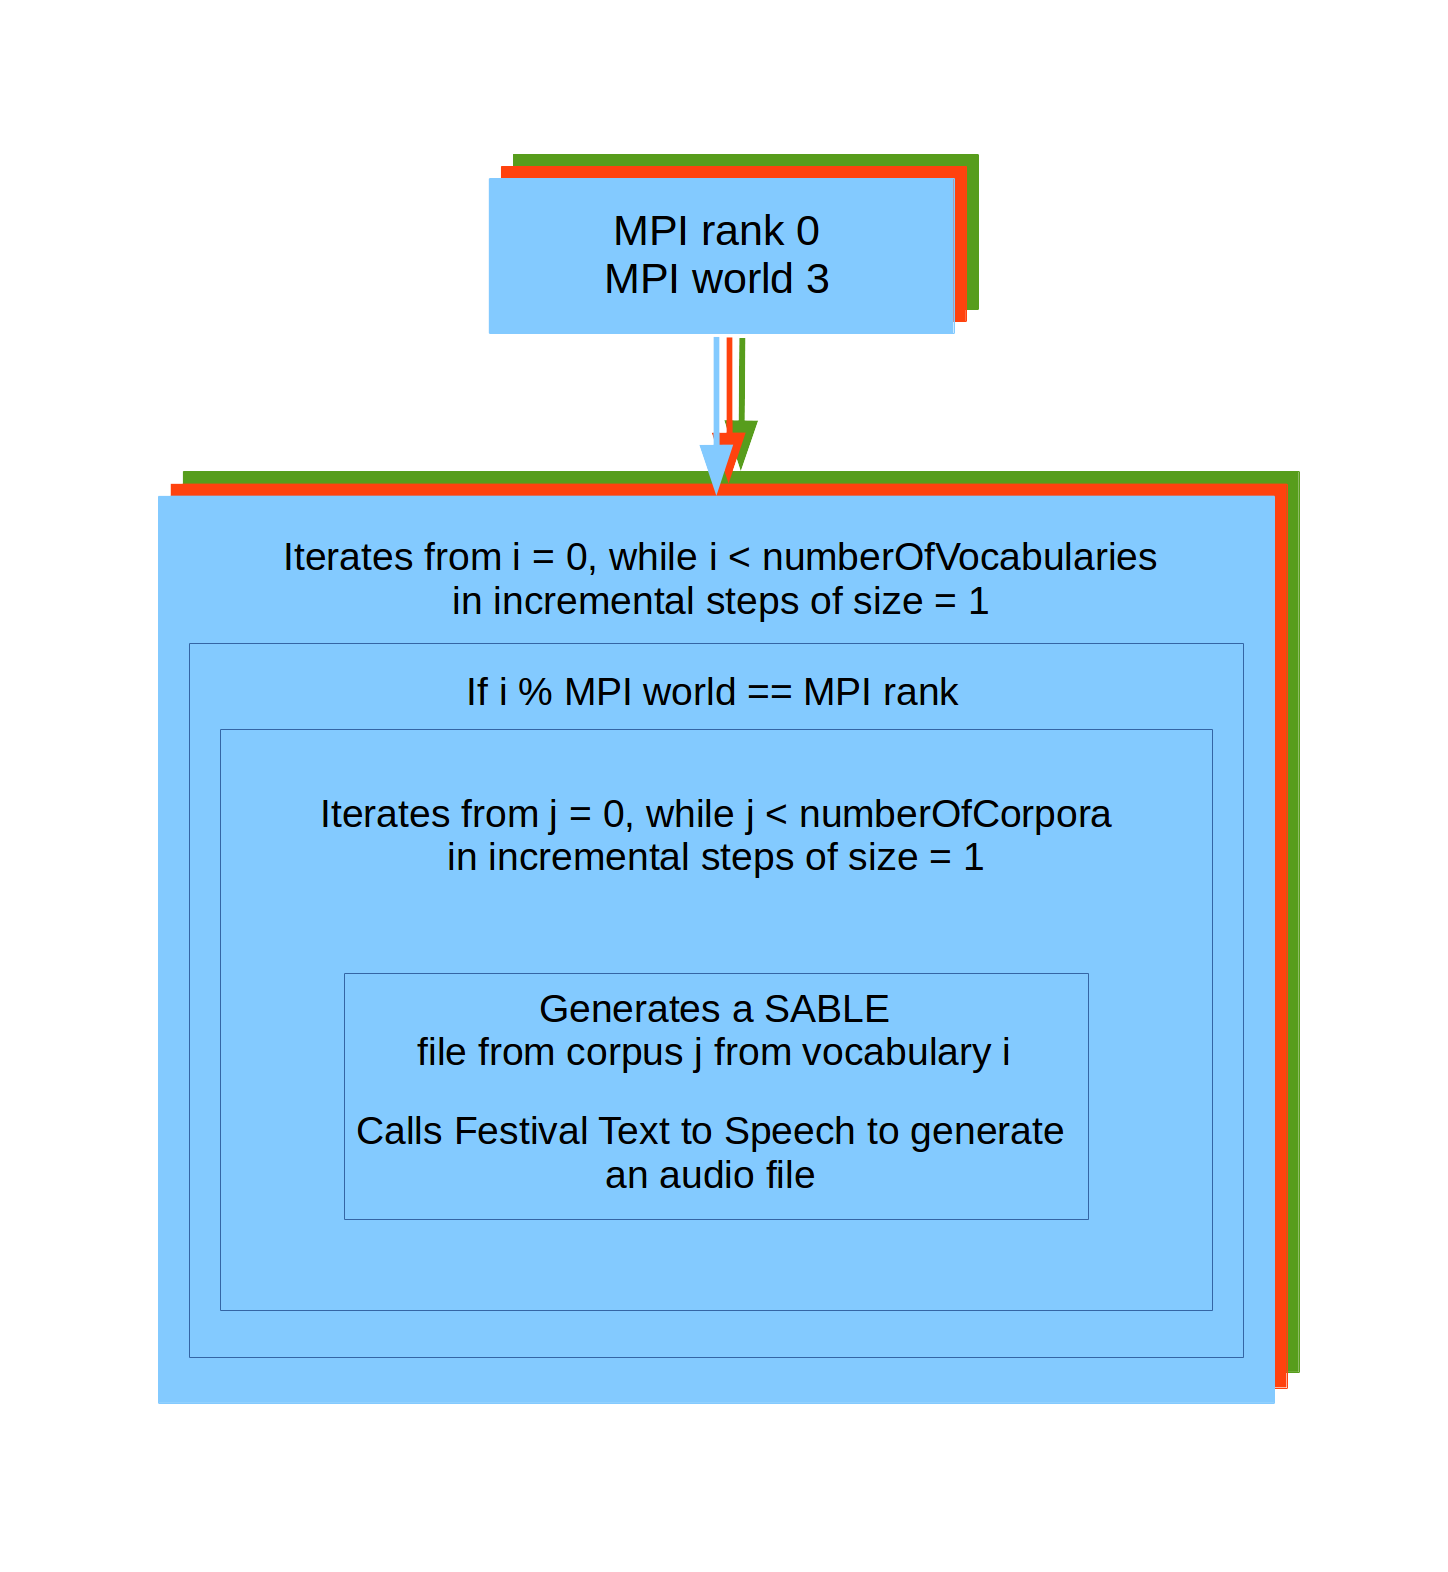
\includegraphics[width=0.482\linewidth]{Corpora_Generation_ALG.png}}
    \hfill
    \subfloat[Vocabularios distribuidos entre procesos \gls{mpi}.\label{sub:CorporaGenerationParallelization}]{%
	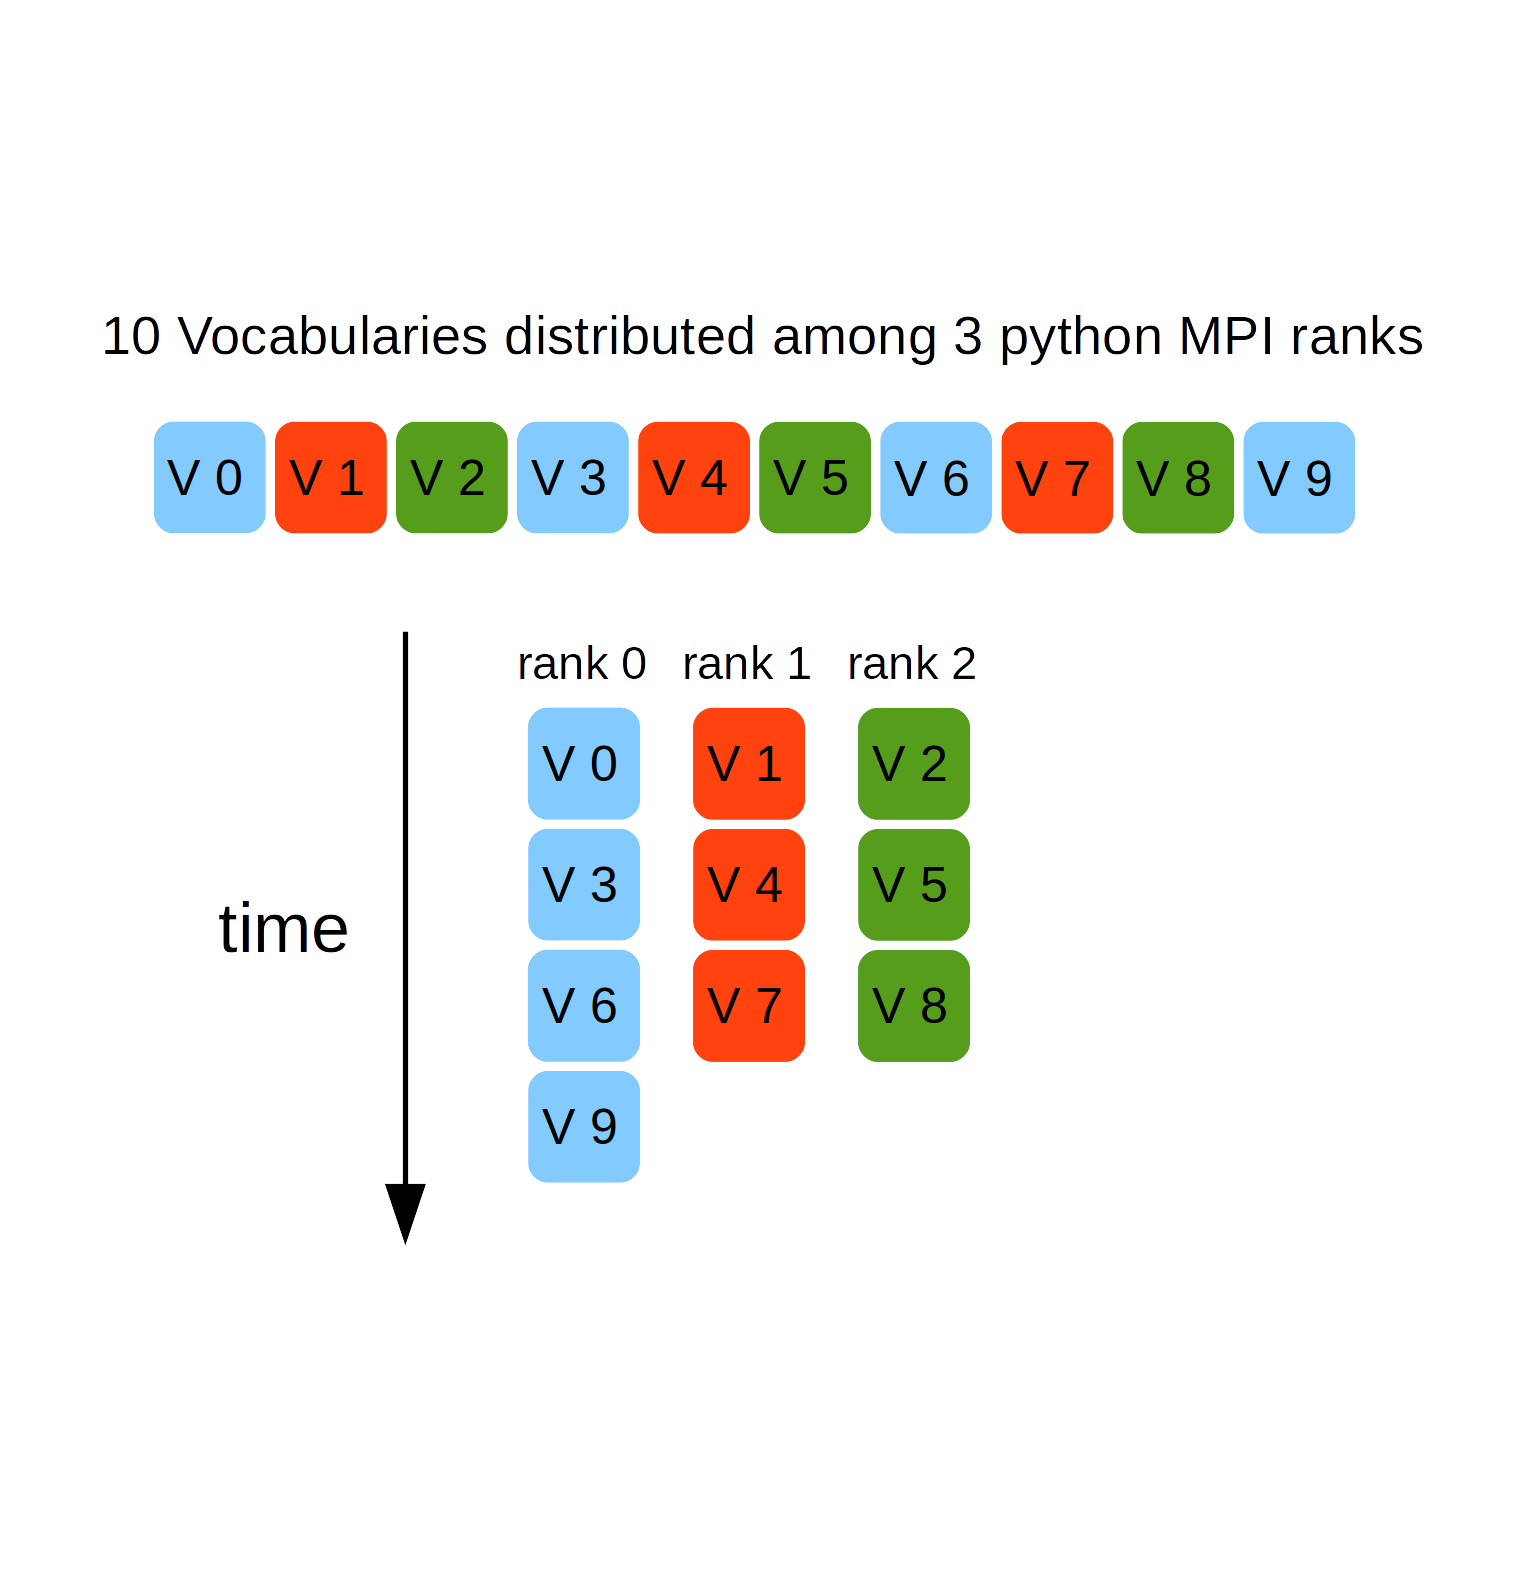
\includegraphics[width=0.482\linewidth]{CorporaGenerationParallelization.png}}
	\caption{Esquema de paralelización para el Proceso de Generación de Corpus.}
  \label{fig:CorporaGenerationParallelization} 
\end{figure*}
}{
\subsection{Corpora Generation Parallel Implementation}
\label{CorpGenImp}

We generated corpora with randomly chosen English mono and multisyllabic words~\cite{10.1371/journal.pone.0217966} using \gls{festival} Synthesis \cite{festival2014}. To that end, we generated cross synthesizer standard mark up language SABLE \cite{sable} files. In those files, we instructed \gls{festival} to generate audio \texttt{wav} files with the corpora uttered by different voices available from the synthesizer.

All the code that generates the corpora is implemented in Python and parallelized by means of an \gls{mpi} package for Python called \texttt{mpi4py}. The algorithmic implementation of this parallelization is shown in Fig.~\ref{fig:CorporaGenerationParallelization}. In such figure, there is a distribution of corpora generation among Python \gls{mpi} ranks. The corpora generation tasks are distributed among ranks as a deck of cards is distributed among players.

In Fig.~\ref{sub:Corpora_Generation_ALG} the parallelization scheme distributes vocabularies among \gls{mpi} processes. In this algorithm we run one \gls{mpi} process per \gls{cpu}. Each rank iterates from 0 to the number of vocabularies minus one with a step size of one. Yet, each rank processes a vocabulary only if the residue of the iteration divided by the number of ranks in the \gls{mpi} environment is equal to the rank identification. In this way, having 10 vocabularies and 3 \gls{mpi} ranks, the rank number 0 will process the vocabularies 0, 3, 6 and 9. All the corpora that corresponds to certain vocabulary are processed serially for the rank which takes charge of such vocabulary.

Fig.~\ref{sub:CorporaGenerationParallelization} shows how each \gls{mpi} rank ends up with a set of vocabularies to generate the corpora corresponding to such vocabularies. If we had 10 corpora per vocabulary, rank 0 would end up generating 40 corpora serially while ranks 1 and 2 would generate 30 corpora each serially.

\begin{figure*}[tb] 
    \centering
  \subfloat[Parallelization algorithm.\label{sub:Corpora_Generation_ALG}]{%
       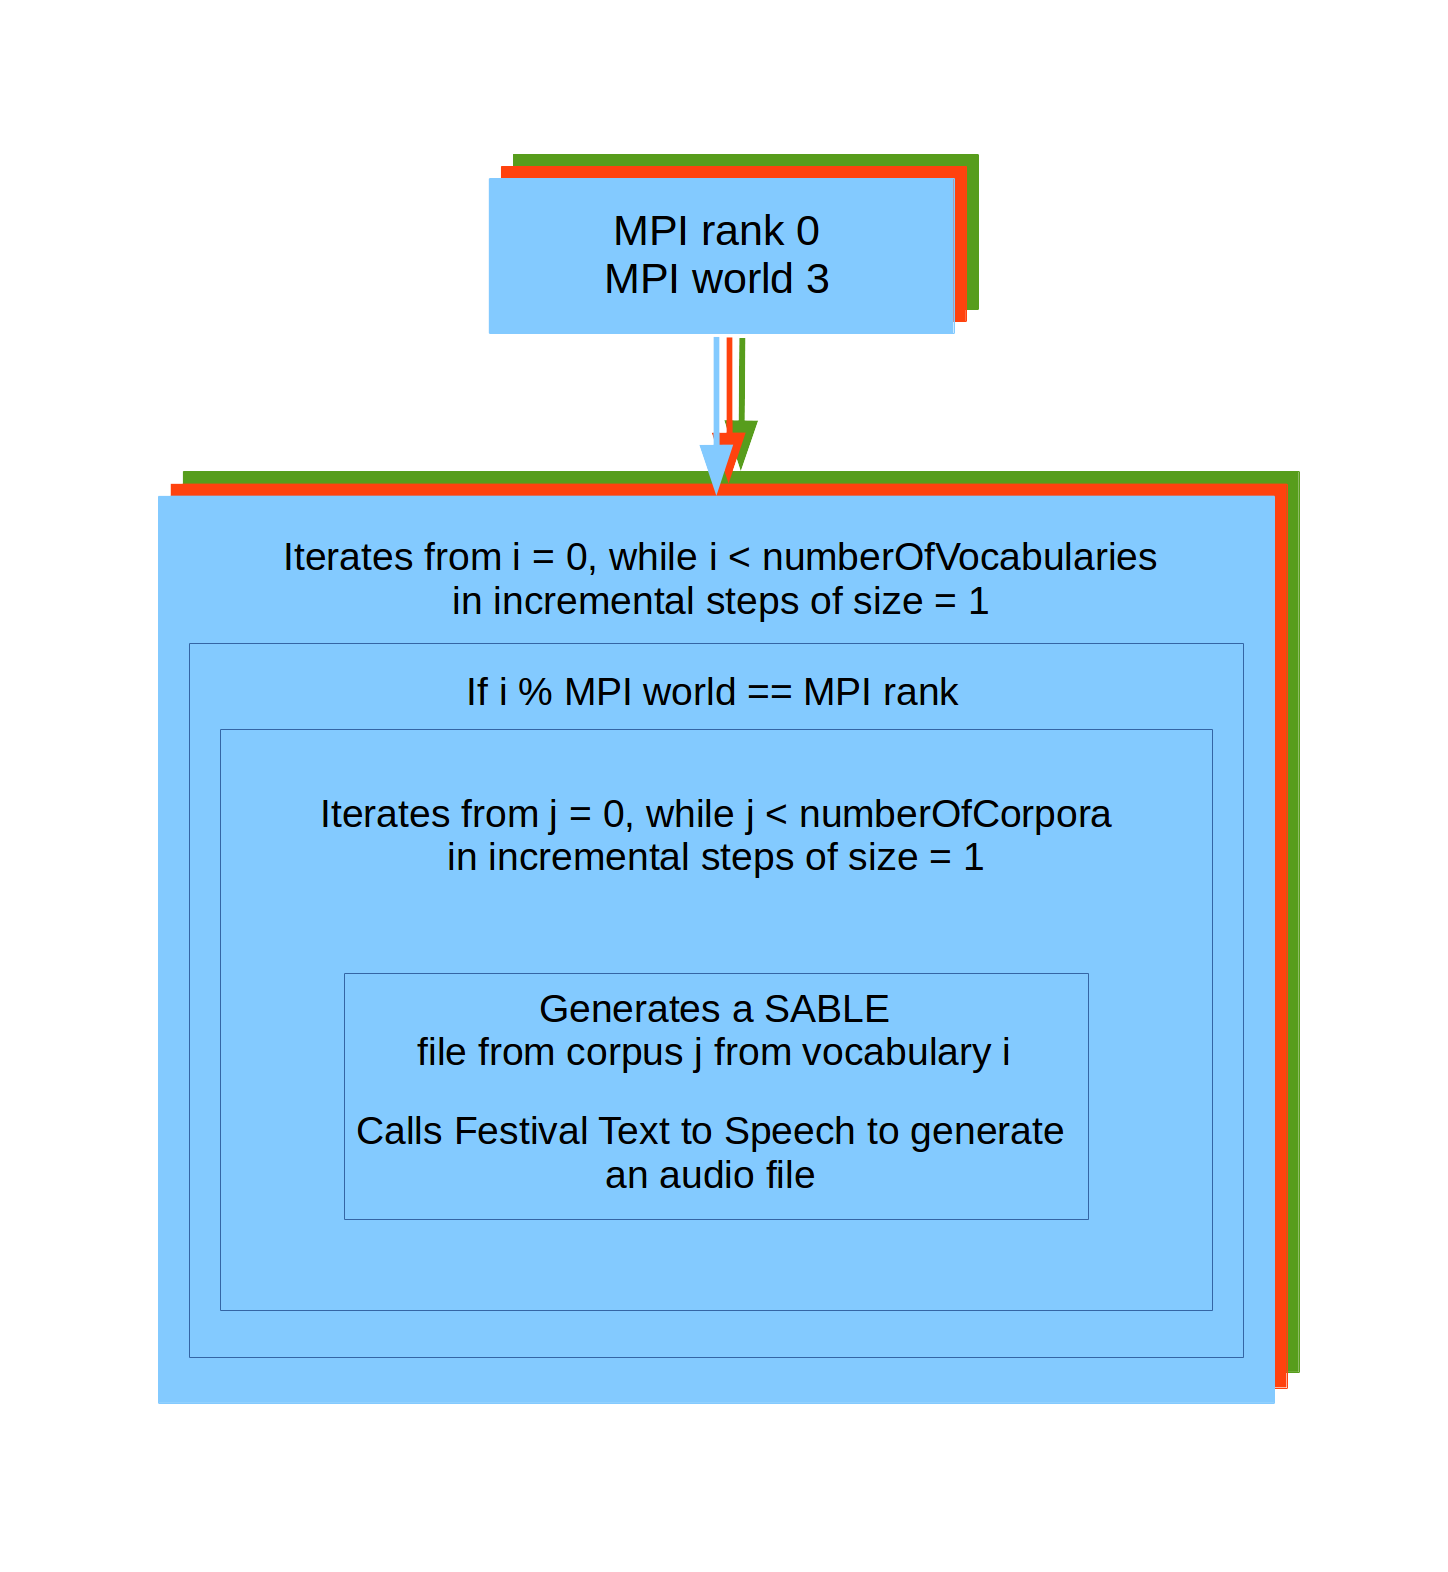
\includegraphics[width=0.482\linewidth]{Corpora_Generation_ALG.png}}
    \hfill
    \subfloat[Vocabularies distributed among \gls{mpi} ranks.\label{sub:CorporaGenerationParallelization}]{%
        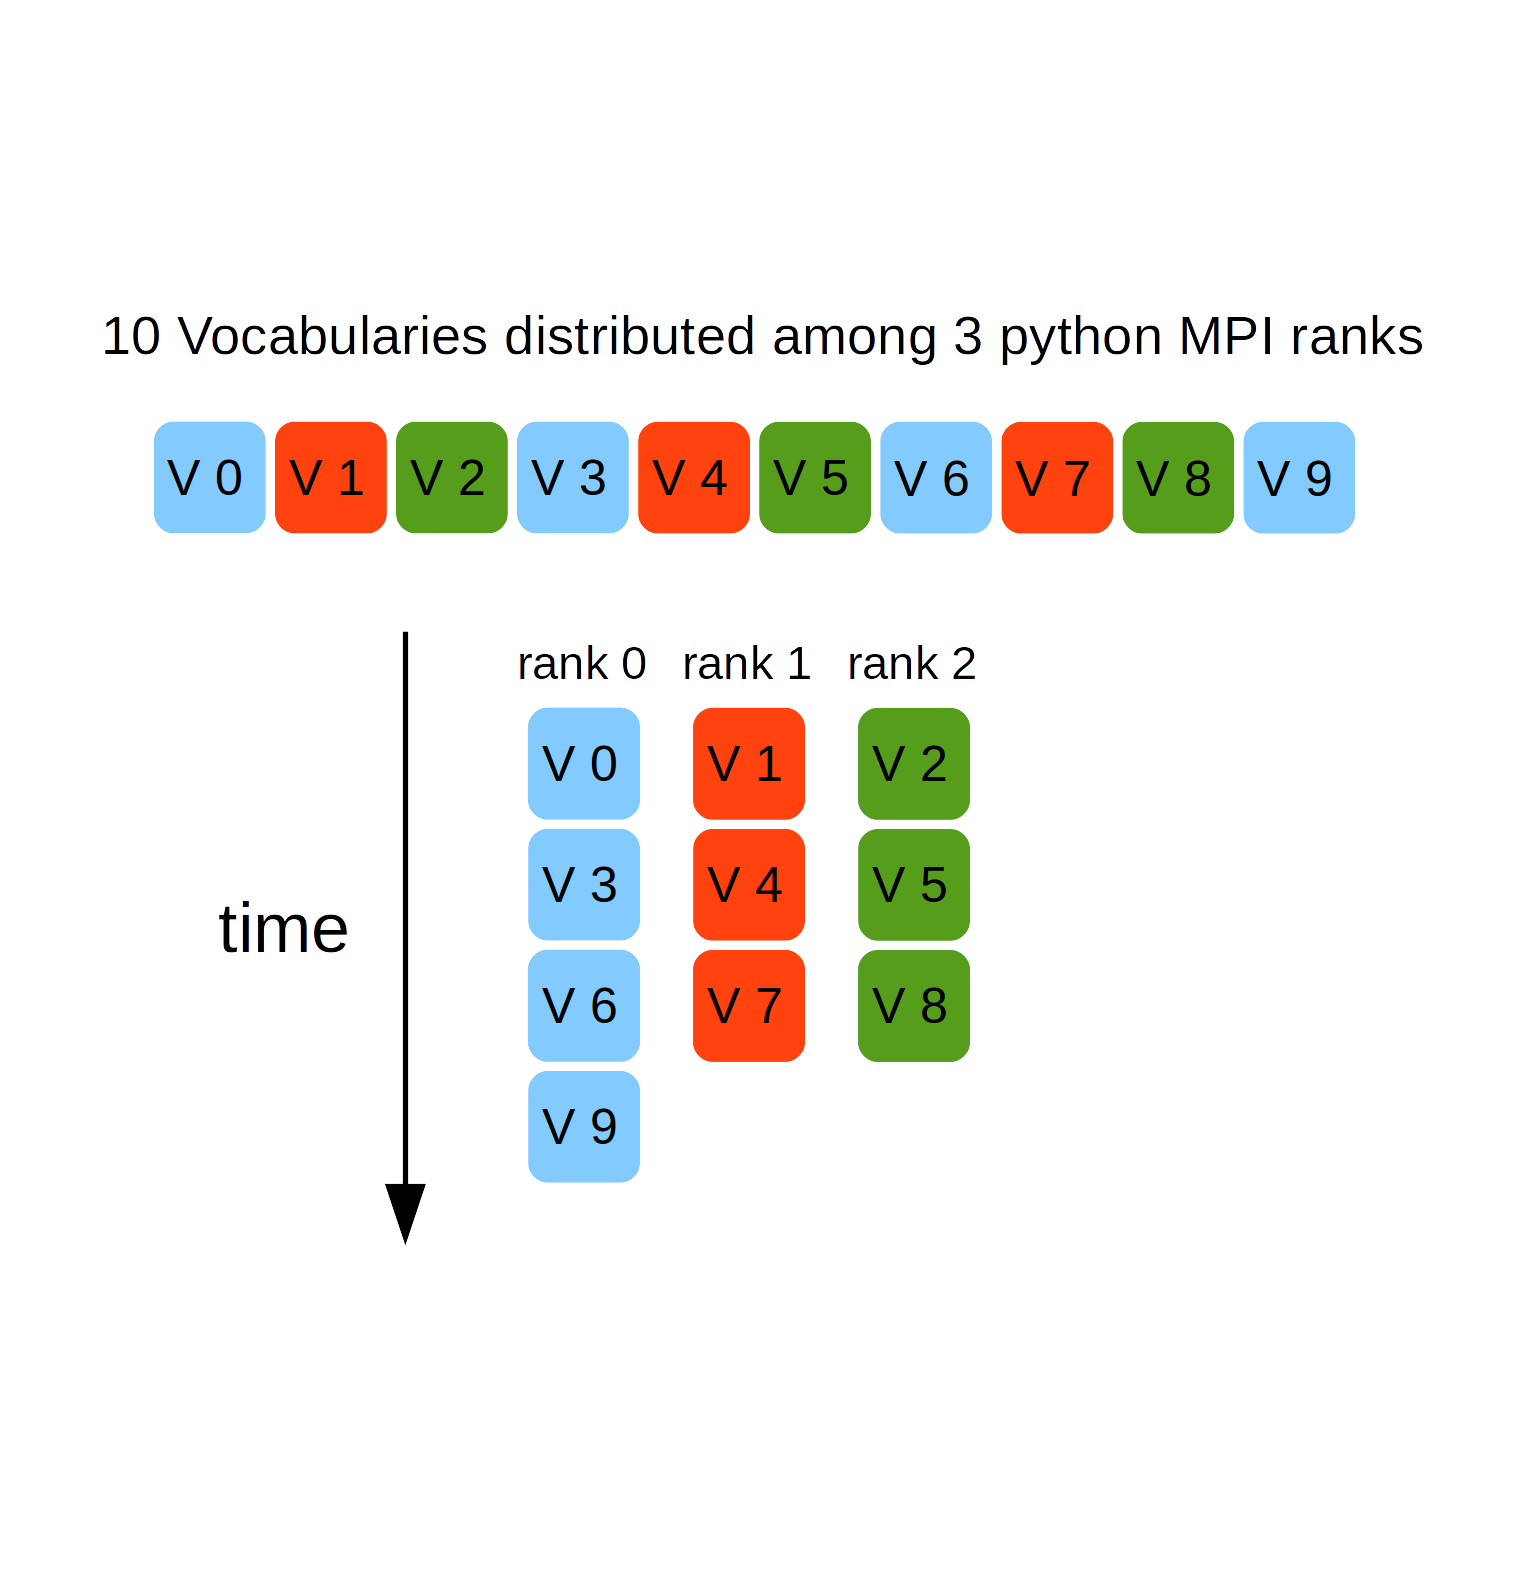
\includegraphics[width=0.482\linewidth]{CorporaGenerationParallelization.png}}
	\caption{Parallelization scheme for the Corpora Generation Process.}
  \label{fig:CorporaGenerationParallelization} 
\end{figure*}
}














\iftoggle{DEBUG}{
\subsection{Implementación Paralela del Análisis Multiresolución Espectro-Temporal de Sonidos (AMRETS)}

Implementamos el algoritmo \gls{mrstsa} en C utilizando el paquete FFTW~\cite{fftw} el cual es una implementación de la \glsfirst{fft} que se encuentra disponible en Cooley.
Utilizamos un enfoque de paralelización híbrido \gls{mpi}+\gls{omp}.
Paralelizamos el algoritmo \gls{mrstsa} desarrollado en D. Dematties et al. \cite{10.1371/journal.pone.0217966} por medio de secciones \gls{omp} utilizando una sección \gls{omp} por resolución espectral corriendo 5 hilos \gls{omp} por nodo.

El esquema de paralelización completo se muestra en la Fig.~\ref{fig:MRSTSA_Parallelization}.
Las tareas son distribuidas entre procesos \gls{mpi} como un mazo de cartas se distribuye entre los distintos jugadores en la partida.
Cada proceso \gls{mpi} termina con un conjunto de tareas las que procesa una a la vez sequencialmente.
Cada tarea es el procesamiento de un corpus que corre 5 hilos \gls{omp} concurrentemente para procesar las resoluciones espectrales.
En este algoritmo corremos un proceso \gls{mpi} por nodo en Cooley.

En relación a \gls{mpi} procesamos un conjunto de corpus por proceso \gls{mpi}.
Suponiendo que tenemos $n$ vocabularios y $m$ corpus por vocabulario, terminamos con $n m$ corpus.
A diferencia del algoritmo de paralelización para la Generación de Corpus expuesto en la Fig.~\ref{sub:Corpora_Generation_ALG} y explicado en la sección~\ref{CorpGenImp}, en este caso desenrollamos el ciclo anidado que itera a través de los corpus y los vocabularios.
El algoritmo de paralelización \gls{mpi}+\gls{omp} se expone en la Fig.~\ref{sub:MRSTSA_ALG}.
En dicho algoritmo, cada proceso itera desde su identificador de proceso hasta el número total de procesos menos uno ($n m - 1$) en pasos incrementales de tamaño igual al número de procesos en el entorno \gls{mpi}.
Para cada iteración (tarea) cada proceso obtiene una identificación de \emph{corpus} y de \emph{vocabulary}, donde los corpus igualan a la división entre la tarea y el número de vocabularios mientras que el vocabulario es igual al resto de la misma división.
Por ejemplo, teniendo tres procesos \gls{mpi} y 10 vocabularios con 1 corpus por vocabulario terminamos teniendo 10 corpus.
En tales condiciones el proceso \gls{mpi} 0 itera a través de las tareas 0, 3, 6 y 9.
Para la tarea 0 corpus es 0 y vocabulario es 0, para la tarea 3 corpus es 0, y vocabulario es 3, para la tarea 6 corpus es 0 y vocabulario es 6, y para la tarea 9 corpus es 0 y vocabulario es 9.
Por otro lado el proceso \gls{mpi} 1 itera a través de las tareas 1, 4 y 7.
Para la tarea 1 corpus es 0 y vocabulario es 1, para la tarea 4 corpus es 0 y vocabulario es 4 y para la tarea 7 corpus es 0 y vocabulario es 7.
Como se puede ver, la estrategia distribuye todos los corpus entre procesos \gls{mpi} y cada proceso \gls{mpi} corre hasta 5 hilos \gls{omp} concurrentemente para generar cada corpus de audio.
La distribución de tareas entre procesos \gls{mpi} en el contexto de 10 vocabularios y 1 corpus por vocabulario se muestra en el Cuadro~\ref{MRSTSA_Tasks_Dist}.

\begin{table*}[tb]
\centering
\caption{Distribución de tareas entre e procesos \gls{mpi} en el contexto de 10 vocabularios y 1 corpus por vocabulario.}
\begin{tabular}{|l|l|l|l|l|l|l|l|l|l|l|}
\hline
Vocabulario & 0                                                       & 1                                                       & 2                                                       & 3                                                       & 4                                                       & 5                                                       & 6                                                       & 7                                                       & 8                                                       & 9                                                       \\ \hline
Corpus 0  & \begin{tabular}[c]{@{}l@{}}proceso 0\\ tarea 0\end{tabular} & \begin{tabular}[c]{@{}l@{}}proceso 1\\ tarea 1\end{tabular} & \begin{tabular}[c]{@{}l@{}}proceso 2\\ tarea 2\end{tabular} & \begin{tabular}[c]{@{}l@{}}proceso 0\\ tarea 3\end{tabular} & \begin{tabular}[c]{@{}l@{}}proceso 1\\ tarea 4\end{tabular} & \begin{tabular}[c]{@{}l@{}}proceso 2\\ tarea 5\end{tabular} & \begin{tabular}[c]{@{}l@{}}proceso 0\\ tarea 6\end{tabular} & \begin{tabular}[c]{@{}l@{}}proceso 1\\ tarea 7\end{tabular} & \begin{tabular}[c]{@{}l@{}}proceso 2\\ tarea 8\end{tabular} & \begin{tabular}[c]{@{}l@{}}proceso 0\\ tarea 9\end{tabular} \\ \hline
\end{tabular}
\label{MRSTSA_Tasks_Dist}
\end{table*}

En la Fig.~\ref{sub:MRSTSA_Parallelization} diez tareas se distribuyen entre procesos \gls{mpi}.
Cada proceso produce una tarea a la vez secuencialmente pero cada resolución espectral del corpus es procesada concurrentemente por medio de hilos \gls{omp}.

Finalmente, el Cuadro~\ref{MRSTSA_Tasks_Dist1} ilustra cómo el esquema de paralelización mostrado en la Fig.~\ref{fig:MRSTSA_Parallelization} distribuiría las tareas entre 3 procesos \gls{mpi} en las condiciones hipotéticas de tener 4 vocabularios y 5 corpus por vocabulario. 

\begin{table}[]
\centering
\caption{Distribución de tareas entre 3 procesos \gls{mpi} en el contexto de 4 vocabularios y 5 corpus por vocabulario.}
\begin{tabular}{|l|l|l|l|l|}
\hline
Vocabulario & 0                                                        & 1                                                        & 2                                                        & 3                                                        \\ \hline
Corpus 0   & \begin{tabular}[c]{@{}l@{}}proceso 0\\ tarea 0\end{tabular}  & \begin{tabular}[c]{@{}l@{}}proceso 1\\ tarea 1\end{tabular}  & \begin{tabular}[c]{@{}l@{}}proceso 2\\ tarea 2\end{tabular}  & \begin{tabular}[c]{@{}l@{}}proceso 0\\ tarea 3\end{tabular}  \\ \hline
Corpus 1   & \begin{tabular}[c]{@{}l@{}}proceso 1\\ tarea 4\end{tabular}  & \begin{tabular}[c]{@{}l@{}}proceso 2\\ tarea 5\end{tabular}  & \begin{tabular}[c]{@{}l@{}}proceso 0\\ tarea 6\end{tabular}  & \begin{tabular}[c]{@{}l@{}}proceso 1\\ tarea 7\end{tabular}  \\ \hline
Corpus 2   & \begin{tabular}[c]{@{}l@{}}proceso 2\\ tarea 8\end{tabular}  & \begin{tabular}[c]{@{}l@{}}proceso 0\\ tarea 9\end{tabular}  & \begin{tabular}[c]{@{}l@{}}proceso 1\\ tarea 10\end{tabular} & \begin{tabular}[c]{@{}l@{}}proceso 2\\ tarea 11\end{tabular} \\ \hline
Corpus 3   & \begin{tabular}[c]{@{}l@{}}proceso 0\\ tarea 12\end{tabular} & \begin{tabular}[c]{@{}l@{}}proceso 1\\ tarea 13\end{tabular} & \begin{tabular}[c]{@{}l@{}}proceso 2\\ tarea 14\end{tabular} & \begin{tabular}[c]{@{}l@{}}proceso 0\\ tarea 15\end{tabular} \\ \hline
Corpus 4   & \begin{tabular}[c]{@{}l@{}}proceso 1\\ tarea 16\end{tabular} & \begin{tabular}[c]{@{}l@{}}proceso 2\\ tarea 17\end{tabular} & \begin{tabular}[c]{@{}l@{}}proceso 0\\ tarea 18\end{tabular} & \begin{tabular}[c]{@{}l@{}}proceso 1\\ tarea 19\end{tabular} \\ \hline
\end{tabular}
\label{MRSTSA_Tasks_Dist1}
\end{table}

\begin{figure*}[tb] 
    \centering
  \subfloat[Algoritmo de Paralelización.\label{sub:MRSTSA_ALG}]{%
       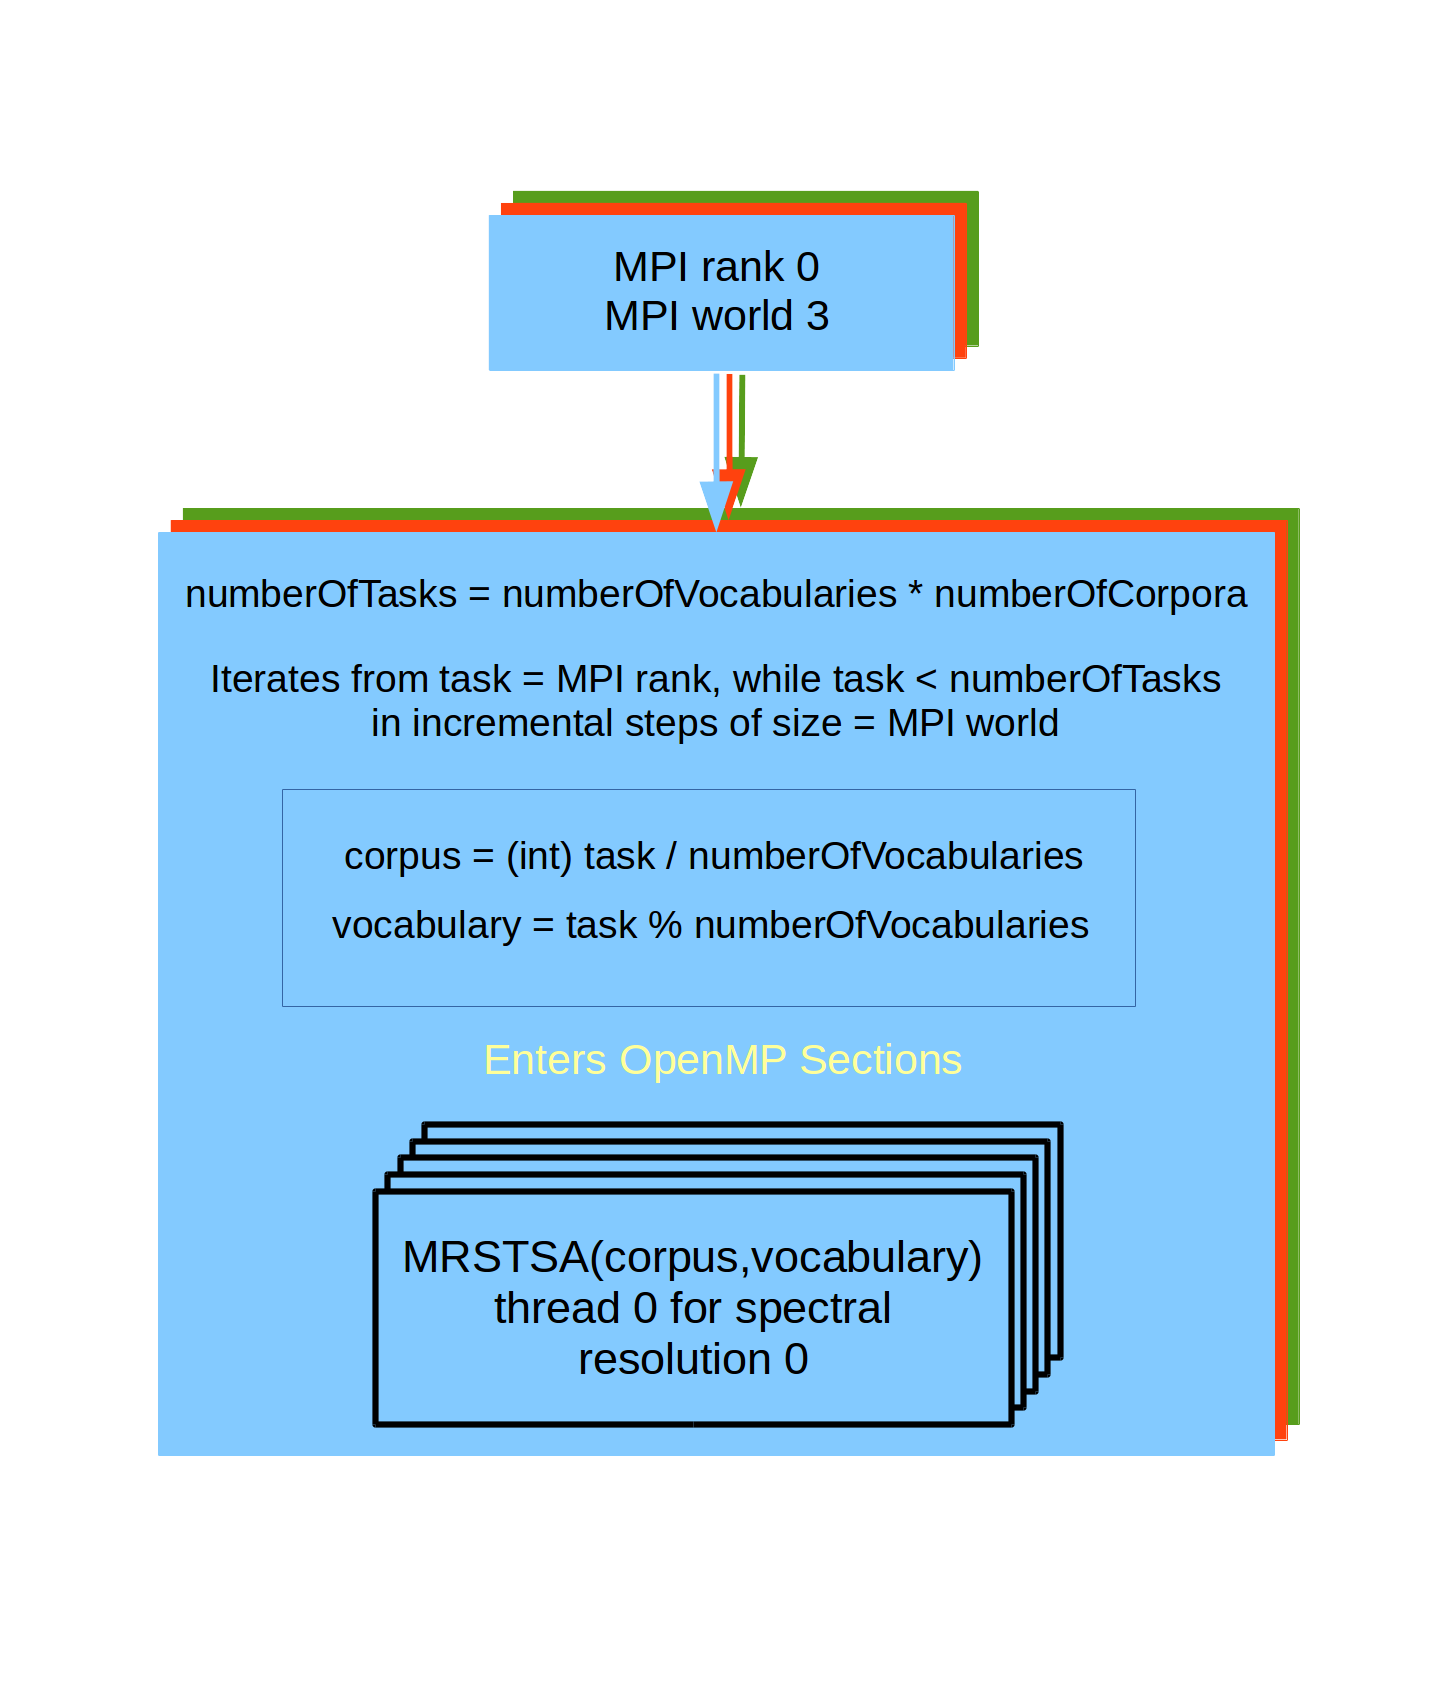
\includegraphics[width=0.482\linewidth]{MRSTSA_ALG.png}}
    \hfill
    \subfloat[Tareas distribuidas entre procesos \gls{mpi}. \label{sub:MRSTSA_Parallelization}]{%
	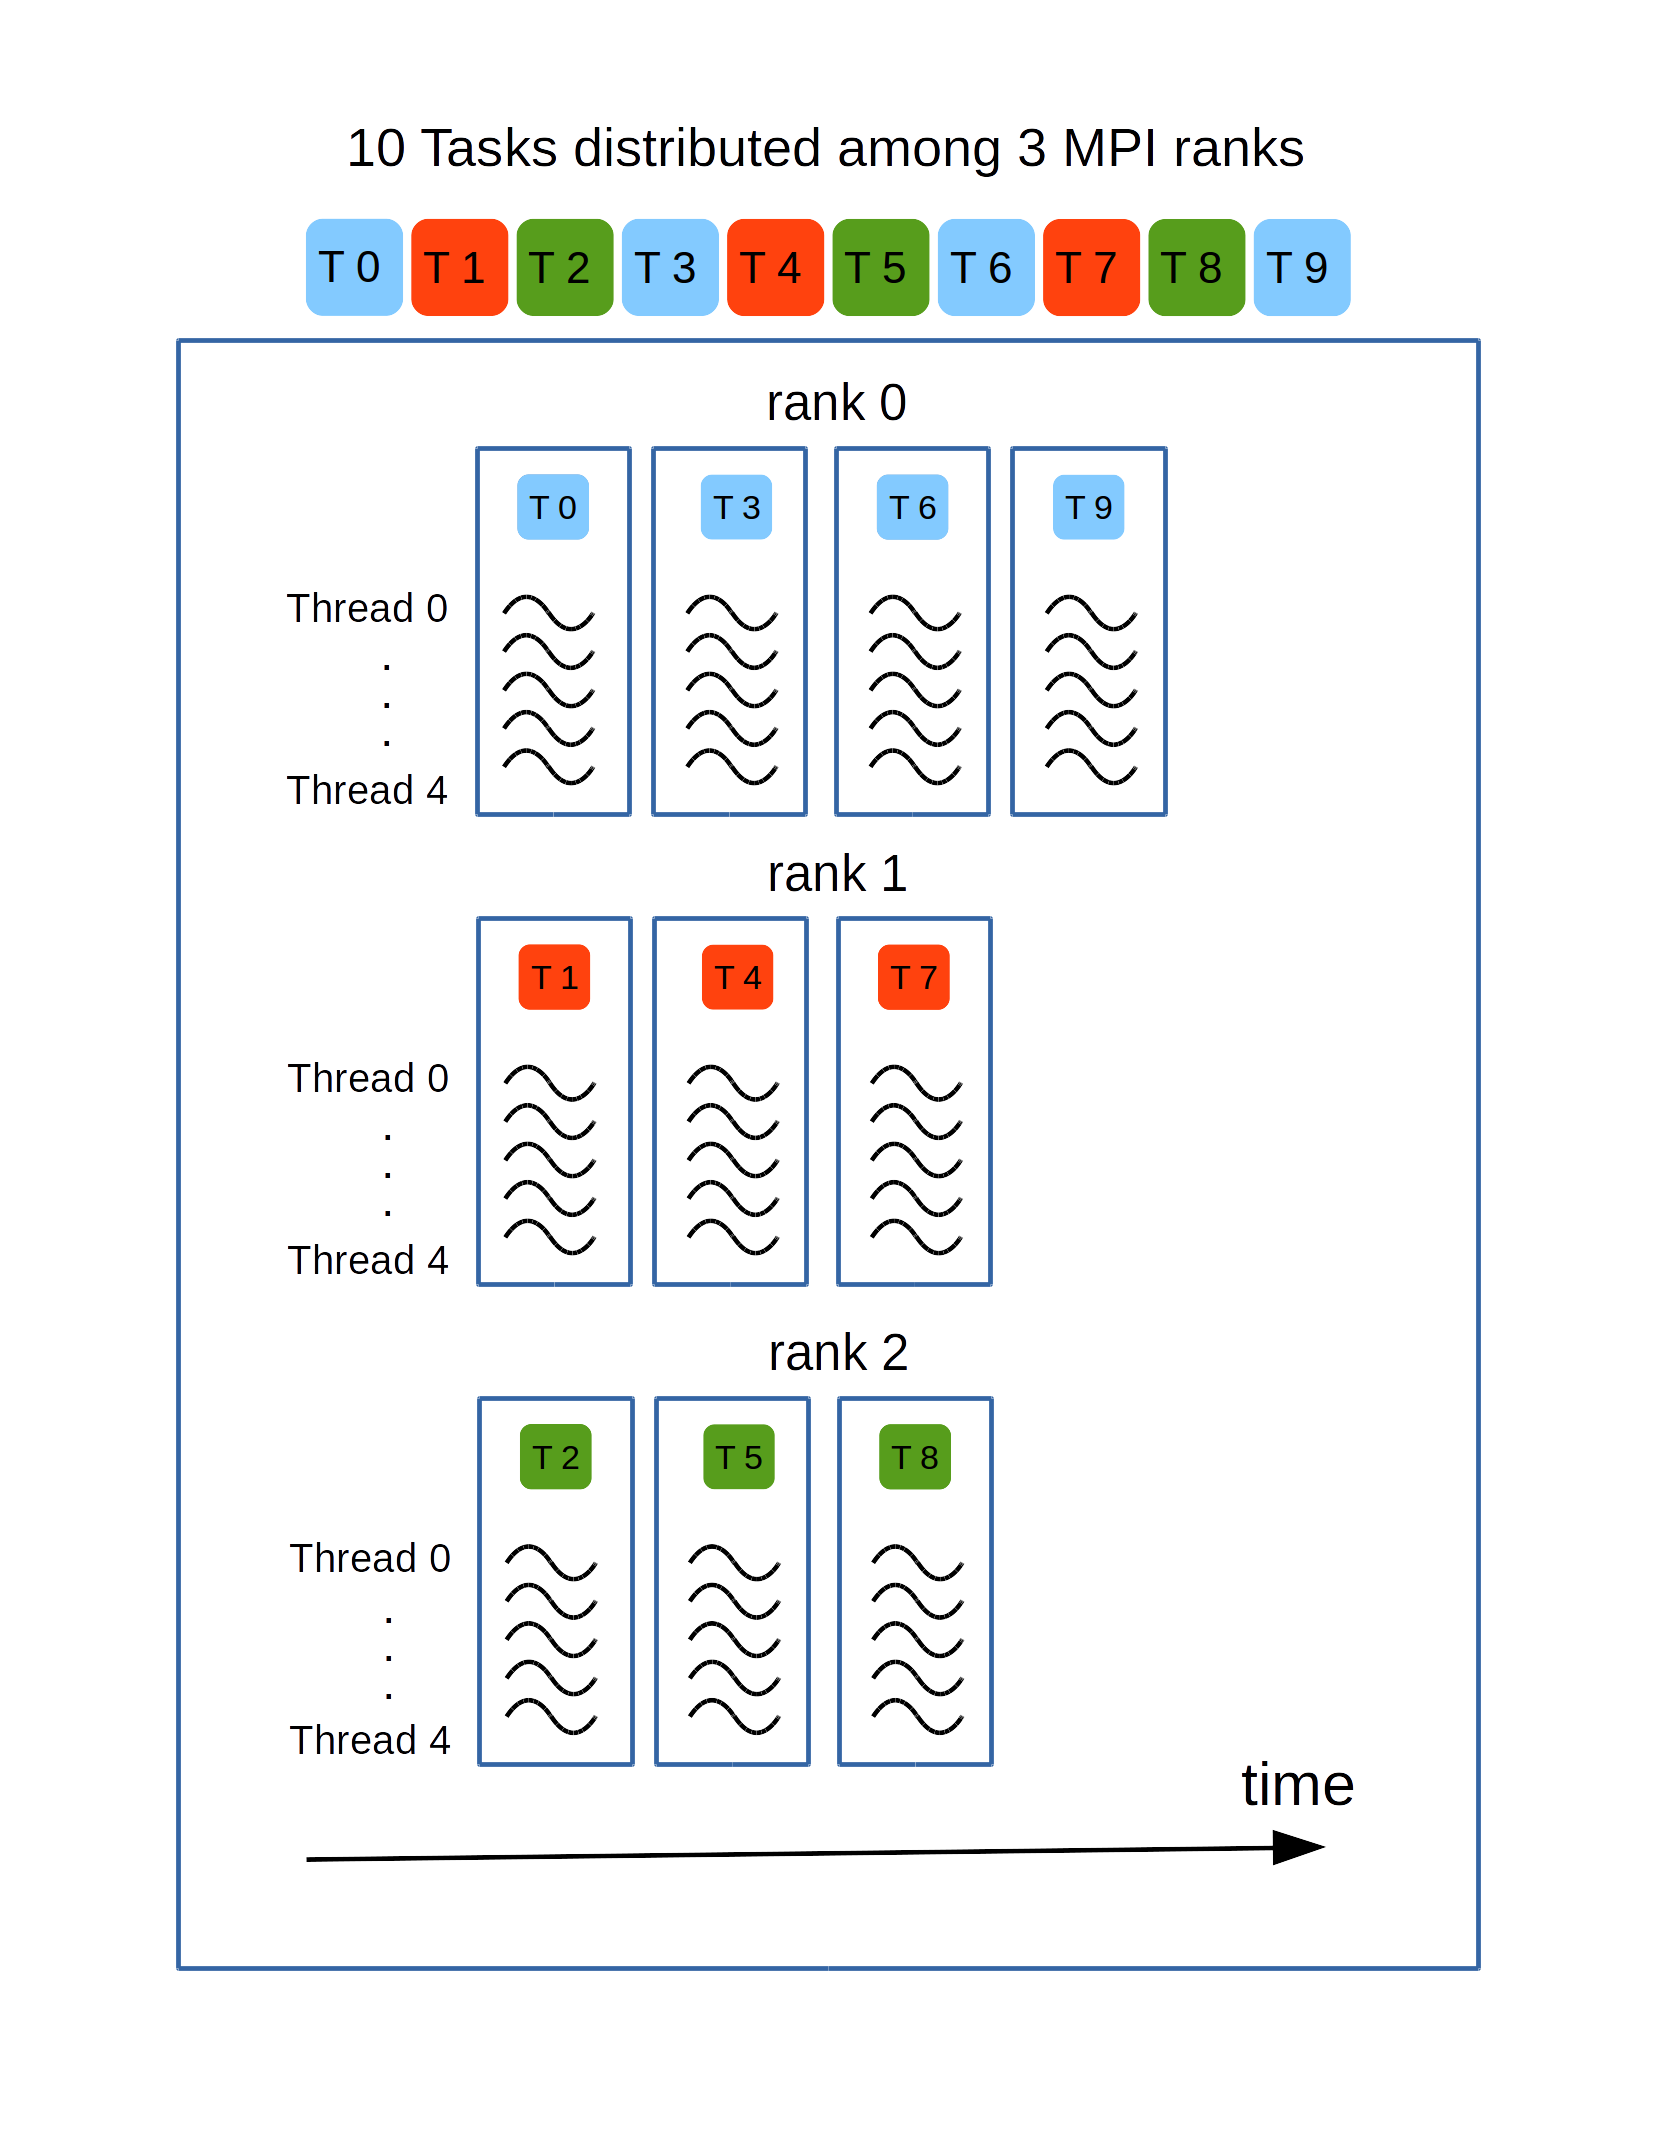
\includegraphics[width=0.482\linewidth]{MRSTSA_Parallelization.png}}
	\caption{Esquema de Paralelización para el \gls{mrstsa}.}
  \label{fig:MRSTSA_Parallelization} 
\end{figure*}
}{
\subsection{Multiresolution Spectro-Temporal Sound Analysis (MRSTSA) Parallel Implementation}

We implemented the \gls{mrstsa} algorithm in C using the package FFTW~\cite{fftw} which is an implementation of the \gls{fft} available on Cooley. We used \gls{mpi}+\gls{omp} hybrid parallelization approach. We parallelized the \gls{mrstsa} algorithm developed in \cite{10.1371/journal.pone.0217966} by means of \gls{omp} sections using one \gls{omp} section per spectral resolution and running until 5 \gls{omp} threads per node.

The complete parallelization scheme is depicted in Fig.~\ref{fig:MRSTSA_Parallelization}. Tasks are distributed among \gls{mpi} ranks as a deck of cards is distributed among players. Each \gls{mpi} rank ends up with a set of tasks which it processes one at a time--sequentially. Each task is a corpus processing which runs 5 \gls{omp} threads concurrently in order to process the spectral resolutions. In this algorithm we run one \gls{mpi} process per Cooley node.% The \gls{mrstsa} algorithm distributes the different spectral resolutions--processing a corpus--among \gls{omp} threads running until 5 \gls{omp} threads concurrently in order to generate such corpus processing.

In terms of \gls{mpi} we processed a set of corpora per \gls{mpi} rank. Supposing that we have $n$ vocabularies and $m$ corpora per vocabulary, we end up with $n m$ corpora. Unlike the Corpora Generation parallelization algorithm exposed in Fig.~\ref{sub:Corpora_Generation_ALG} and explained in section~\ref{CorpGenImp}, in this case we unroll the nested loop that iterates through corpora and vocabularies. The \gls{mpi}+\gls{omp} parallelization algorithm is exposed in Fig.~\ref{sub:MRSTSA_ALG}. In this algorithm, each rank iterates from the rank identification to the number of tasks minus one ($n m - 1$) in incremental steps of size equal to the number of ranks in the \gls{mpi} environment. For each iteration (task) each rank obtains a \emph{corpus} and a \emph{vocabulary} identification, where the corpus equals the division between the task and the number of vocabularies while the vocabulary is the residue from the same division. For example, having three \gls{mpi} ranks and 10 vocabularies with 1 corpus per vocabulary we end up having 10 corpora. In such conditions the \gls{mpi} rank 0 would iterate through tasks 0, 3, 6 and 9. For task 0 corpus is 0 and vocabulary is 0, for task 3 corpus is 0, and vocabulary is 3, for task 6 corpus is 0 and vocabulary is 6, and for task 9 corpus is 0 and vocabulary is 9. On the other hand \gls{mpi} rank 1 iterates through tasks 1, 4 and 7. For task 1 corpus is 0 and vocabulary is 1, for task 4 corpus is 0 and vocabulary is 4 and for task 7 corpus is 0 and vocabulary is 7. As can be seen the strategy distributes all the corpora among \gls{mpi} processes and each \gls{mpi} process runs until 5 \gls{omp} threads concurrently in order to generate each audio corpus. The distribution of tasks among \gls{mpi} ranks in the context of 10 vocabularies and 1 corpus per vocabulary is shown in Table~\ref{MRSTSA_Tasks_Dist}. 

\begin{table*}[tb]
\centering
\caption{Distribution of tasks among 3 \gls{mpi} ranks in the context of 10 vocabularies and 1 corpus per vocabulary.}
\begin{tabular}{|l|l|l|l|l|l|l|l|l|l|l|}
\hline
Vocabulary & 0                                                       & 1                                                       & 2                                                       & 3                                                       & 4                                                       & 5                                                       & 6                                                       & 7                                                       & 8                                                       & 9                                                       \\ \hline
Corpus 0  & \begin{tabular}[c]{@{}l@{}}rank 0\\ task 0\end{tabular} & \begin{tabular}[c]{@{}l@{}}rank 1\\ task 1\end{tabular} & \begin{tabular}[c]{@{}l@{}}rank 2\\ task 2\end{tabular} & \begin{tabular}[c]{@{}l@{}}rank 0\\ task 3\end{tabular} & \begin{tabular}[c]{@{}l@{}}rank 1\\ task 4\end{tabular} & \begin{tabular}[c]{@{}l@{}}rank 2\\ task 5\end{tabular} & \begin{tabular}[c]{@{}l@{}}rank 0\\ task 6\end{tabular} & \begin{tabular}[c]{@{}l@{}}rank 1\\ task 7\end{tabular} & \begin{tabular}[c]{@{}l@{}}rank 2\\ task 8\end{tabular} & \begin{tabular}[c]{@{}l@{}}rank 0\\ task 9\end{tabular} \\ \hline
\end{tabular}
\label{MRSTSA_Tasks_Dist}
\end{table*}

In Fig.~\ref{sub:MRSTSA_Parallelization} ten tasks are distributed among \gls{mpi} ranks. Each rank processes one task at a time sequentially but each corpus spectral resolution is processed concurrently by means of \gls{omp} threads.

Finally, Table~\ref{MRSTSA_Tasks_Dist1} depicts how the parallelization scheme shown in Fig.~\ref{fig:MRSTSA_Parallelization} would distribute tasks among 3 \gls{mpi} ranks in the hypothetic conditions of having 4 vocabularies and 5 corpora per vocabulary.

\begin{table}[]
\centering
\caption{Distribution of tasks among 3 \gls{mpi} ranks in the context of 4 vocabularies and 5 corpora per vocabulary.}
\begin{tabular}{|l|l|l|l|l|}
\hline
Vocabulary & 0                                                        & 1                                                        & 2                                                        & 3                                                        \\ \hline
Corpus 0   & \begin{tabular}[c]{@{}l@{}}rank 0\\ task 0\end{tabular}  & \begin{tabular}[c]{@{}l@{}}rank 1\\ task 1\end{tabular}  & \begin{tabular}[c]{@{}l@{}}rank 2\\ task 2\end{tabular}  & \begin{tabular}[c]{@{}l@{}}rank 0\\ task 3\end{tabular}  \\ \hline
Corpus 1   & \begin{tabular}[c]{@{}l@{}}rank 1\\ task 4\end{tabular}  & \begin{tabular}[c]{@{}l@{}}rank 2\\ task 5\end{tabular}  & \begin{tabular}[c]{@{}l@{}}rank 0\\ task 6\end{tabular}  & \begin{tabular}[c]{@{}l@{}}rank 1\\ task 7\end{tabular}  \\ \hline
Corpus 2   & \begin{tabular}[c]{@{}l@{}}rank 2\\ task 8\end{tabular}  & \begin{tabular}[c]{@{}l@{}}rank 0\\ task 9\end{tabular}  & \begin{tabular}[c]{@{}l@{}}rank 1\\ task 10\end{tabular} & \begin{tabular}[c]{@{}l@{}}rank 2\\ task 11\end{tabular} \\ \hline
Corpus 3   & \begin{tabular}[c]{@{}l@{}}rank 0\\ task 12\end{tabular} & \begin{tabular}[c]{@{}l@{}}rank 1\\ task 13\end{tabular} & \begin{tabular}[c]{@{}l@{}}rank 2\\ task 14\end{tabular} & \begin{tabular}[c]{@{}l@{}}rank 0\\ task 15\end{tabular} \\ \hline
Corpus 4   & \begin{tabular}[c]{@{}l@{}}rank 1\\ task 16\end{tabular} & \begin{tabular}[c]{@{}l@{}}rank 2\\ task 17\end{tabular} & \begin{tabular}[c]{@{}l@{}}rank 0\\ task 18\end{tabular} & \begin{tabular}[c]{@{}l@{}}rank 1\\ task 19\end{tabular} \\ \hline
\end{tabular}
\label{MRSTSA_Tasks_Dist1}
\end{table}

\begin{figure*}[tb] 
    \centering
  \subfloat[Parallelization algorithm.\label{sub:MRSTSA_ALG}]{%
       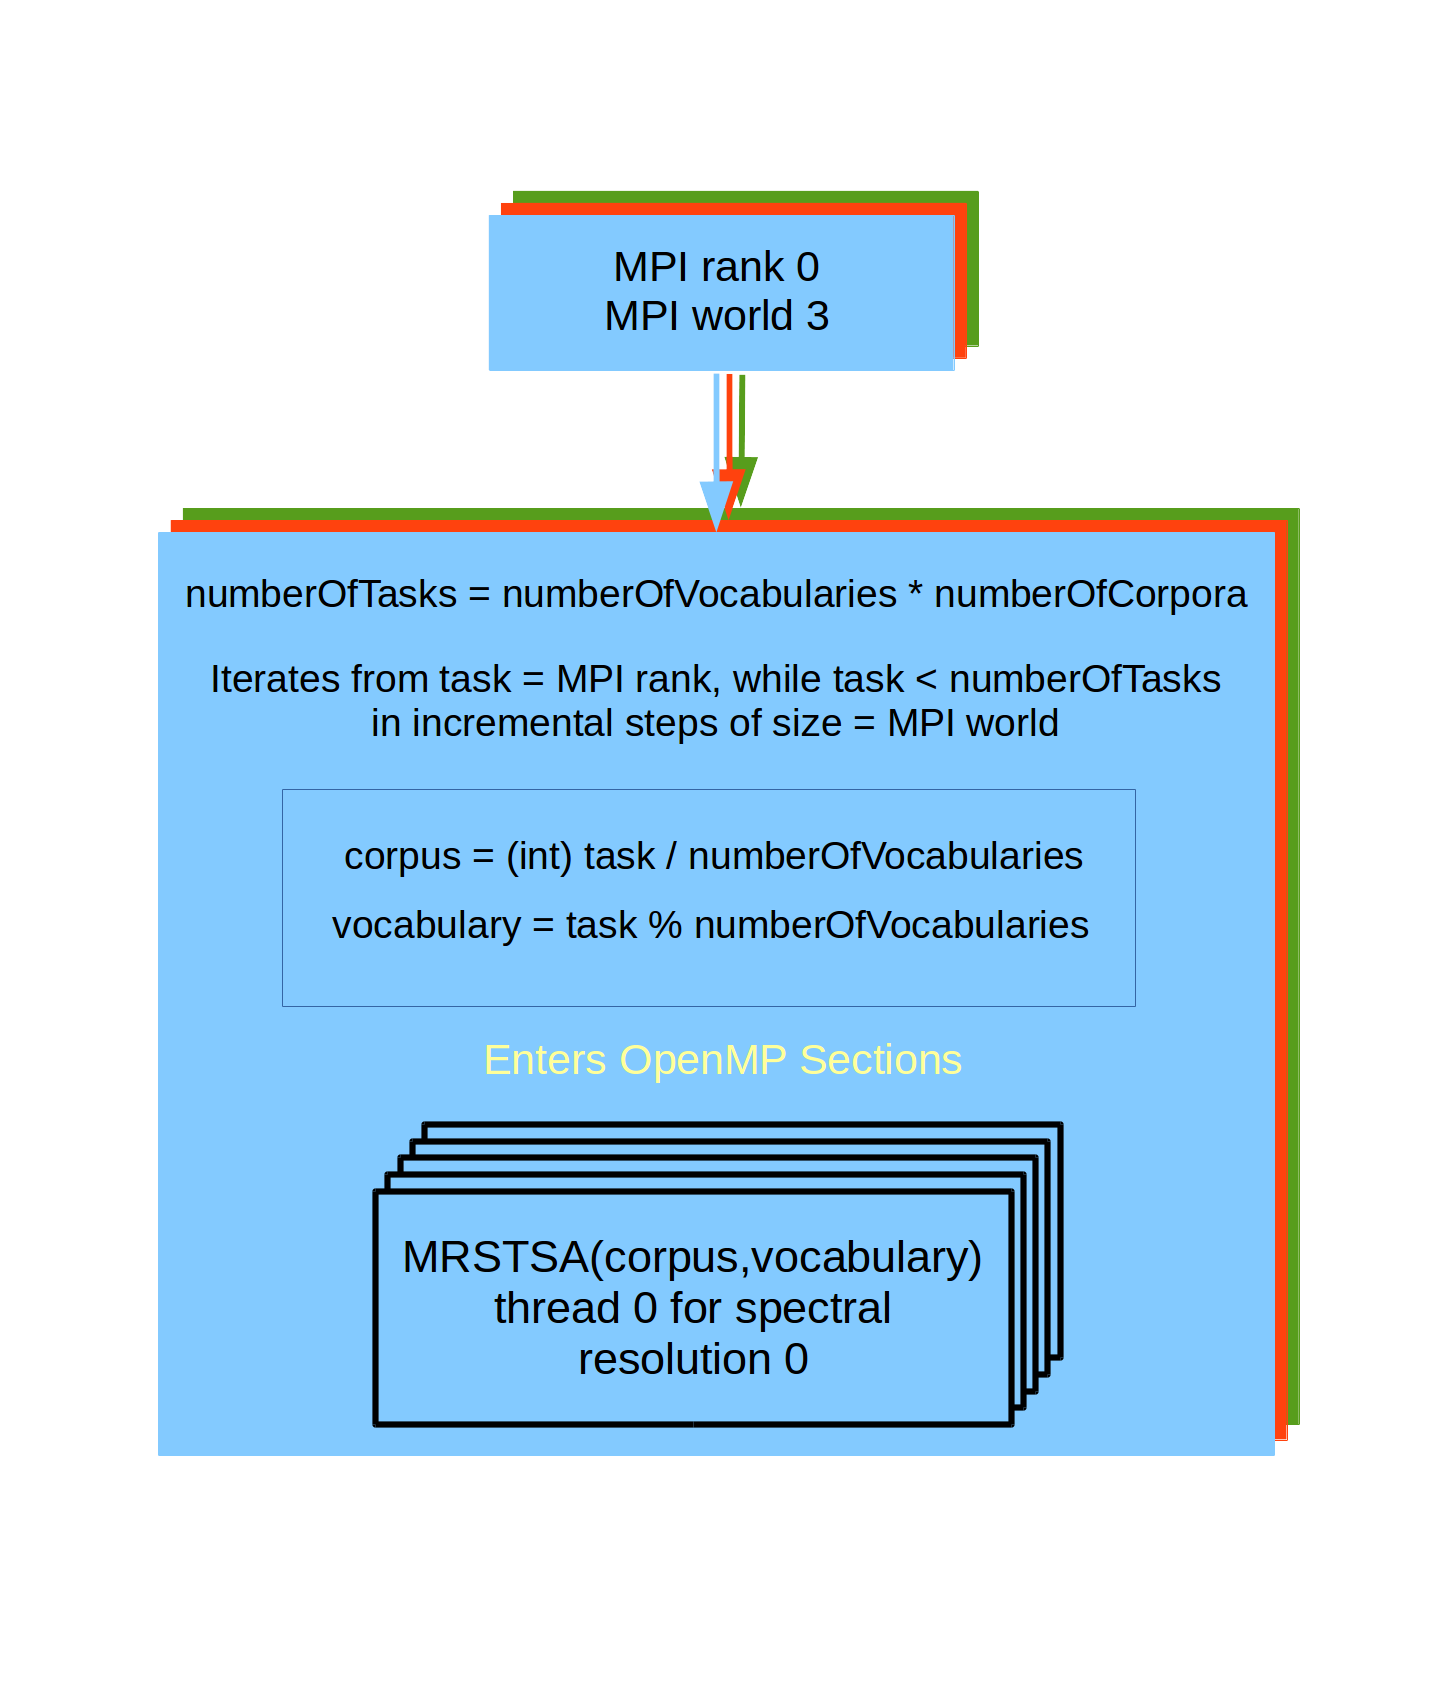
\includegraphics[width=0.482\linewidth]{MRSTSA_ALG.png}}
    \hfill
    \subfloat[Tasks distributed among \gls{mpi} ranks.\label{sub:MRSTSA_Parallelization}]{%
        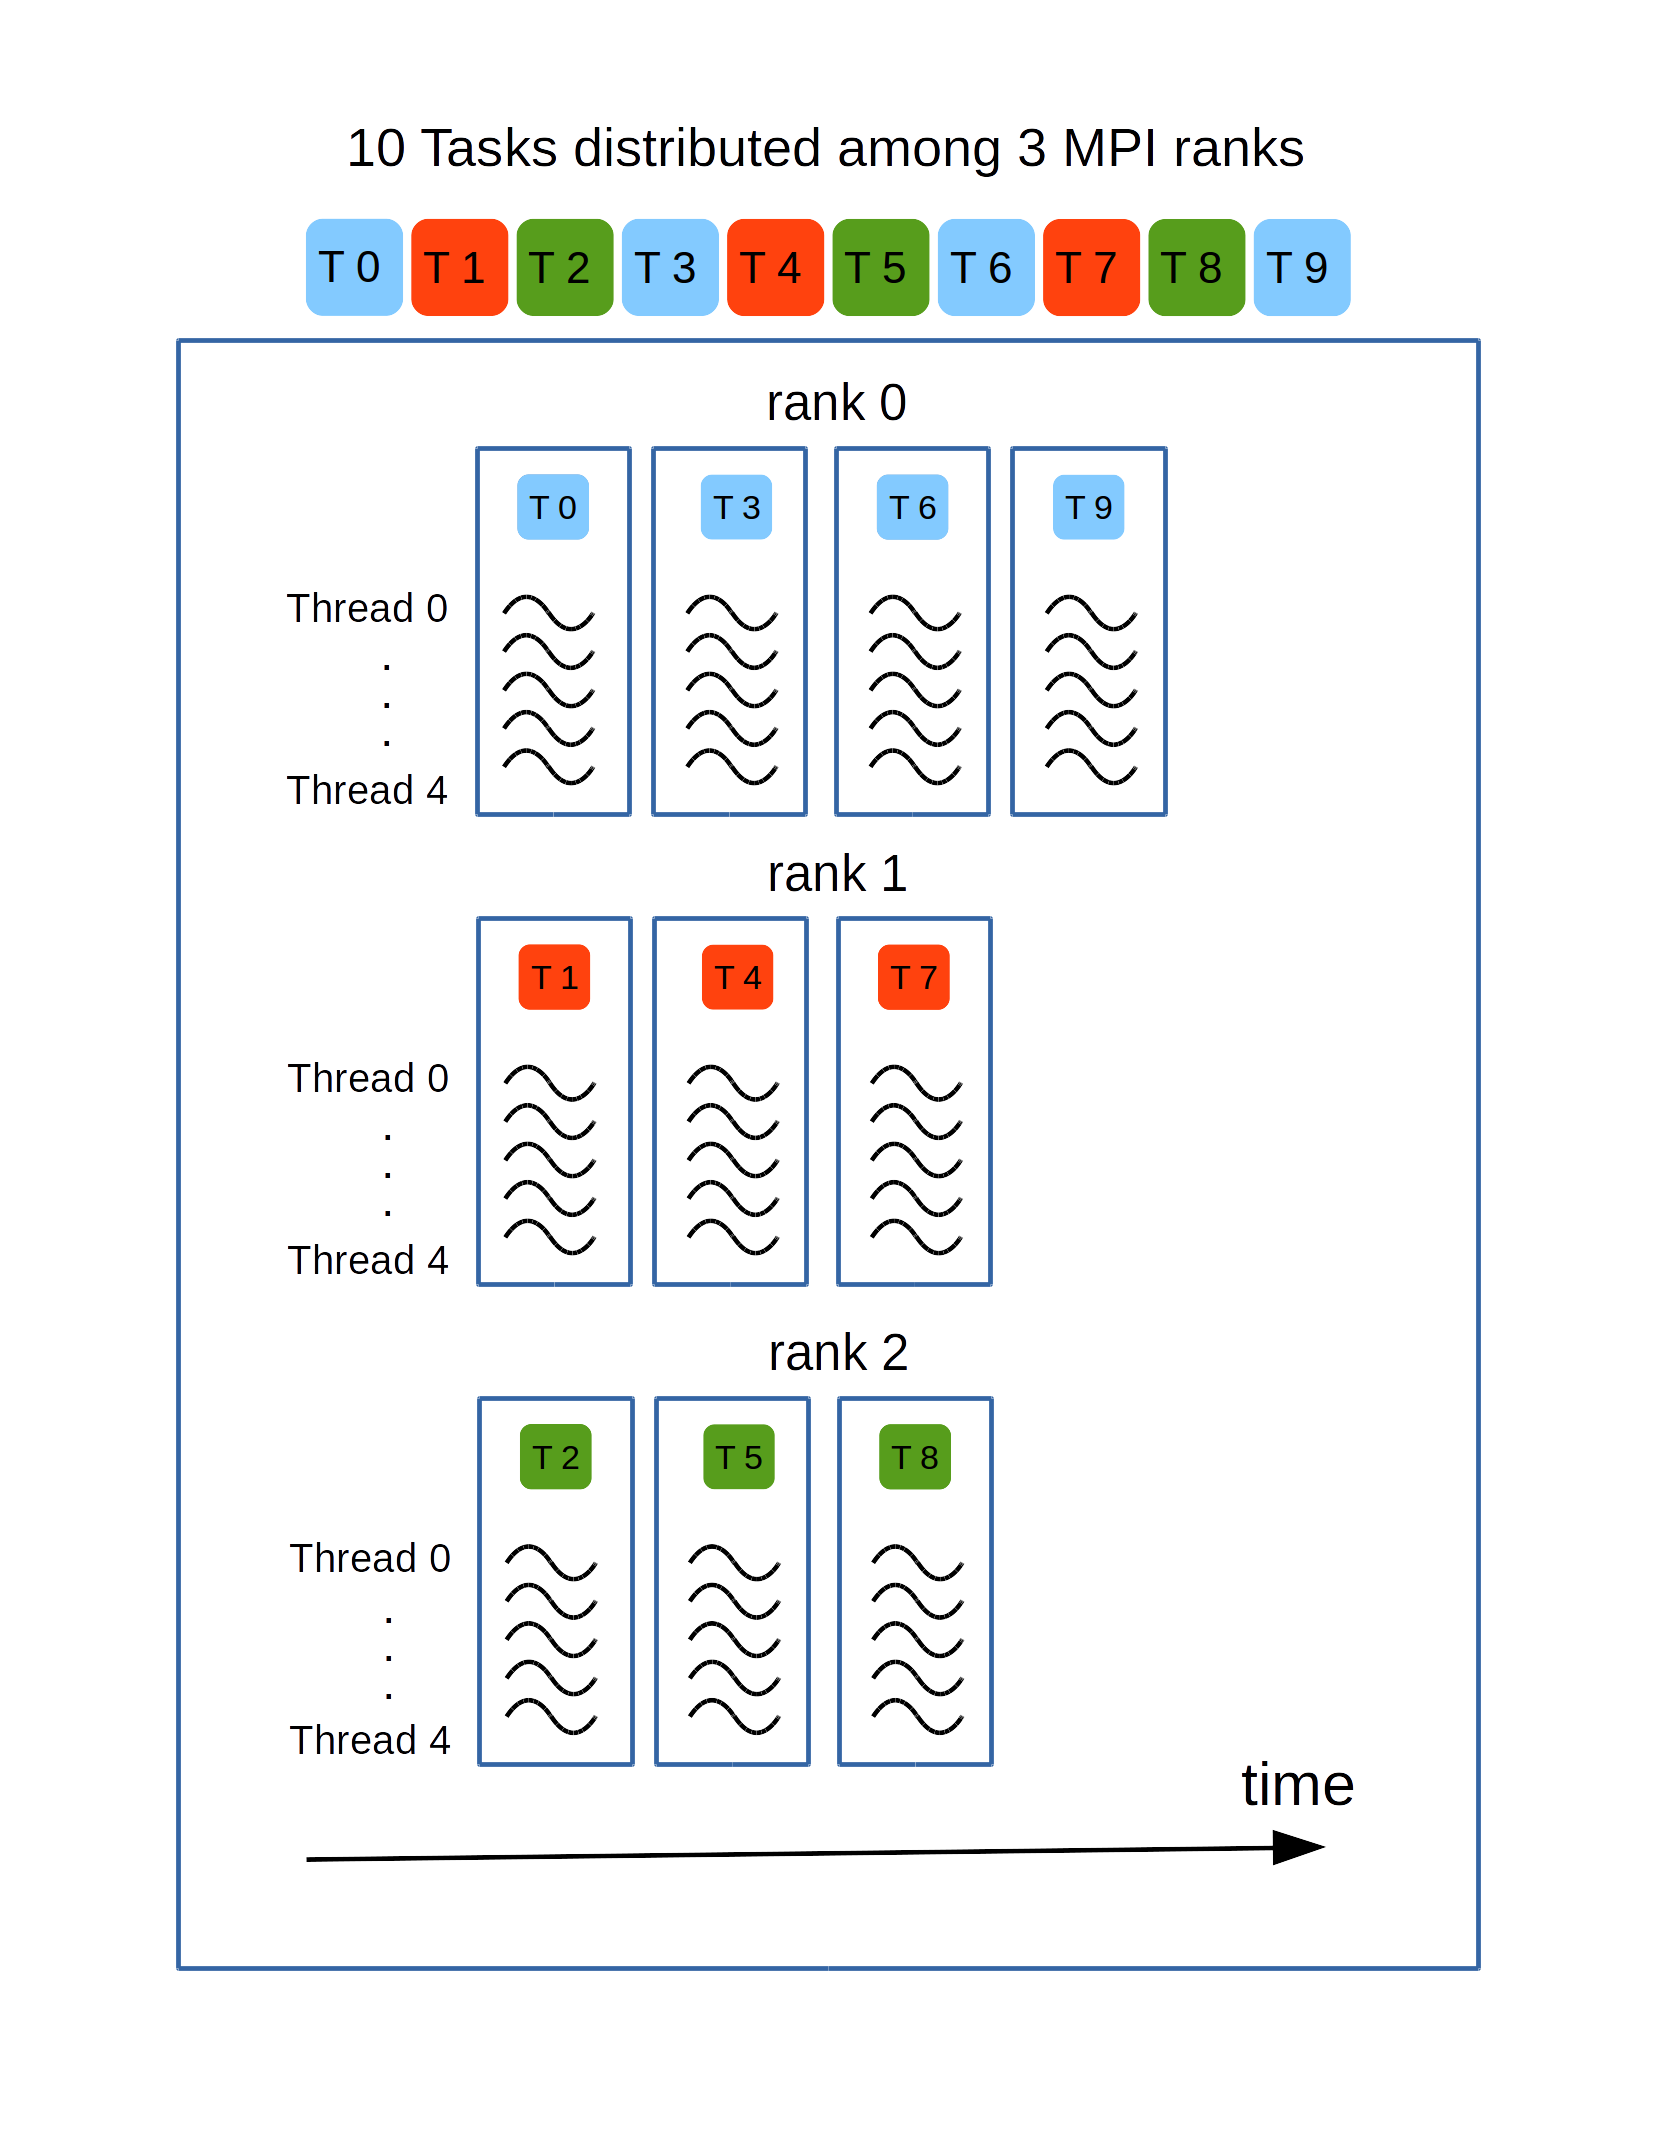
\includegraphics[width=0.482\linewidth]{MRSTSA_Parallelization.png}}
	\caption{Parallelization scheme for the \gls{mrstsa}.}
  \label{fig:MRSTSA_Parallelization} 
\end{figure*}
}


















\iftoggle{DEBUG}{
\subsection{Implementación Paralela de la \glsfirst{el}}
\label{EL_Parallelization}

La \gls{el} simula un parche de tejido cortical e incorpora organización columnar, formación espontánea micro-columnar, depolarización parcial \gls{nmda} y adaptación a activaciones contextuales.
Simulamos células piramidales segregando las conexiones próximas--desde ramas dendríticas aferentes--completamente de las conexiones distales--desde ramas dendríticas laterales.
Este algoritmo produce \gls{sdr_pl} que el cerebro utiliza para procesar información en todos los mamíferos, desde ratones hasta humanos~\cite{barth_2012}.

Paralelizamos la \gls{el} por medio de un paradigma híbrido \gls{mpi}+\gls{omp} distribuyendo \glsfirst{csom_pl} entre procesos \gls{mpi} como un mazo de cartas se distribuye entre los diferentes jugadores de la partida.
Cada proceso \gls{mpi} termina con uno o más \gls{csom_pl} y los \gls{csom_pl} en cada proceso se distribuyen entre diferentes hilos \gls{omp}.

La Fig.~\ref{fig:Encoder_Parallelization} muestra la distribución de objetos \gls{csom_pl} en una \gls{el} con 3 por 8 (24) \gls{cc_pl} en tres procesos \gls{mpi} con tres hilos \gls{omp} cada uno.
Ciertos procesos podrían hacerse cargo de un número diferente de \gls{csom_pl} dependiendo del número de procesos \gls{mpi} así como del número de \gls{cc_pl} en la \gls{el}.
Cada proceso \gls{mpi} distribuye sus \gls{csom_pl} entre diferentes hilos de la misma manera.

\begin{figure}[h!]
    \centering
    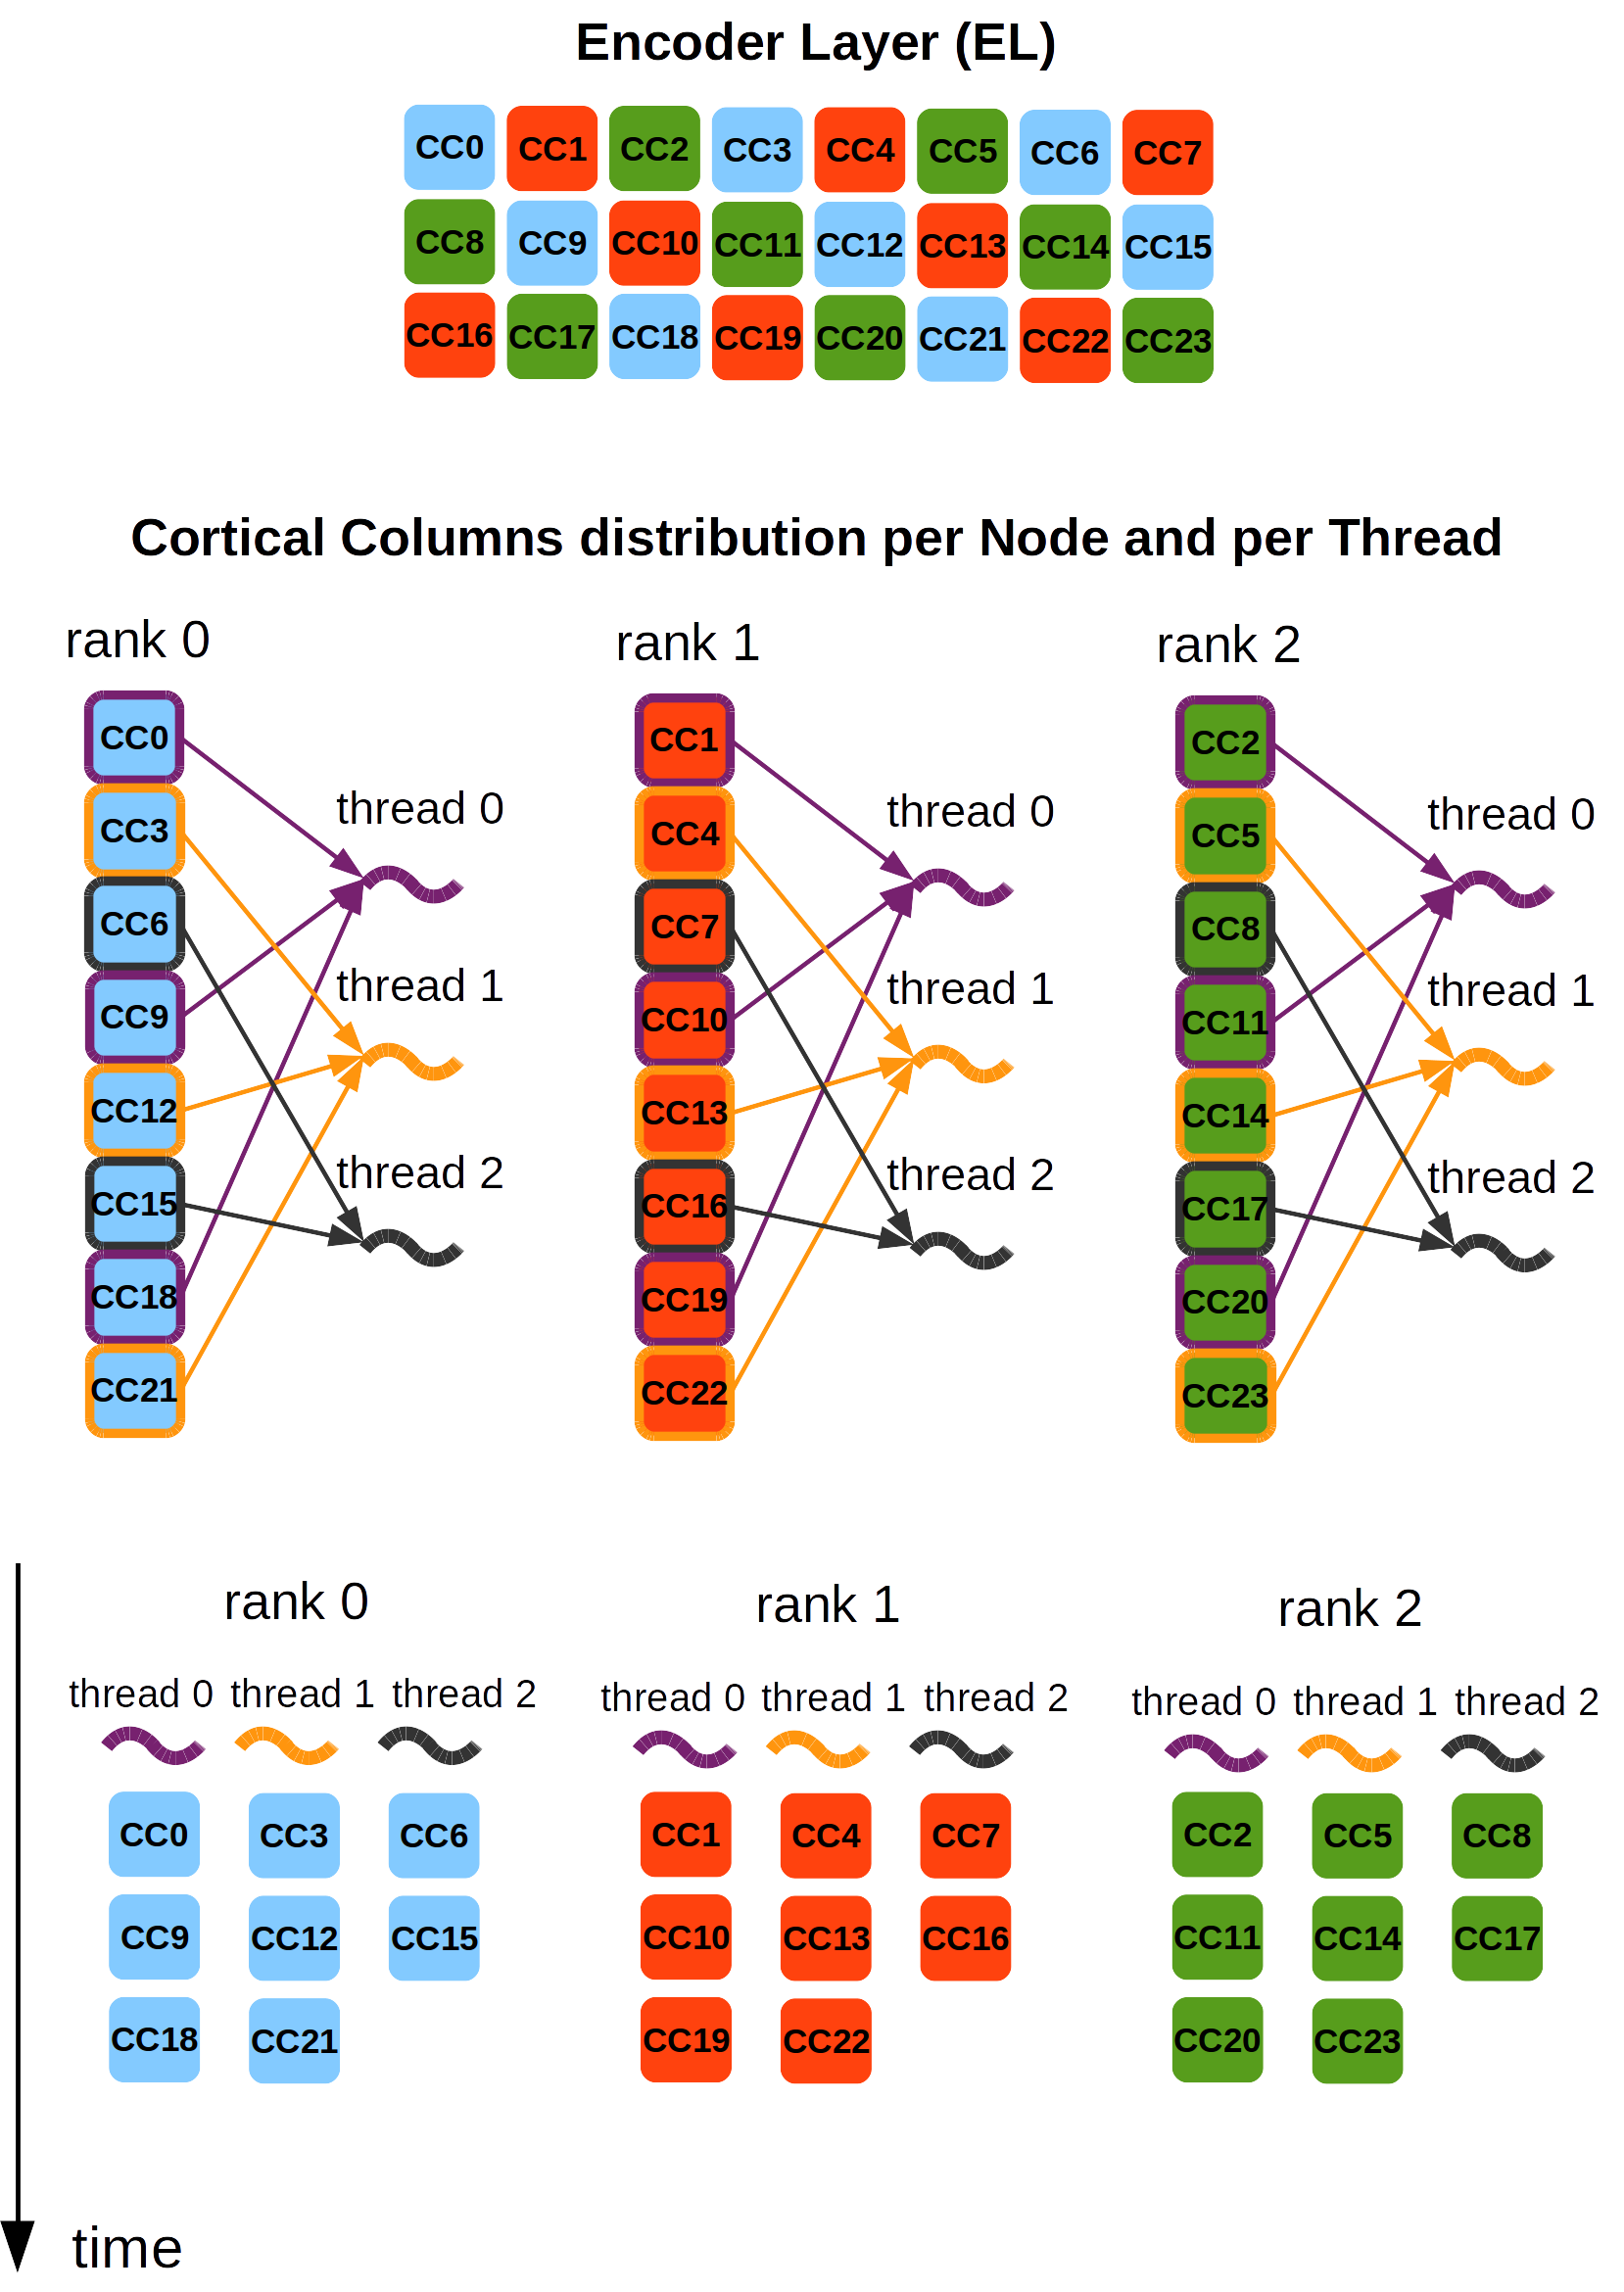
\includegraphics[width=0.7\textwidth]{Encoder_Parallelization.png}
    \caption{Paralelización \gls{mpi}+\gls{omp} de la \gls{el}.}
    \label{fig:Encoder_Parallelization}
\end{figure}

La información entre los procesos \gls{mpi} se debe transferir en cada paso temporal.
Básicamente toda la información requerida por cada proceso es la identidad de las unidades neuronales activas en cada \gls{cc} de la \gls{el}.
Agrupamos toda la información correspondiente a los \gls{csom_pl} en cada proceso y luego utilizamos la función \gls{mpi} Bcast para transmitir tal información usando un protocolo de comunicación especial por medio del cual especificamos los límites de la información correspondiente a cada \gls{csom}.
Por medio de esta estrategia cada proceso \gls{mpi} tiene que llamar \gls{mpi} Bcast solo una vez para transmitir sus datos.

La Fig. \ref{fig:BCast} muestra que la \gls{ipc} se lleva a cabo en cada paso temporal ya que cada proceso \gls{mpi} requiere la salida completa desde la \gls{el} en cada paso temporal.
Cada proceso \gls{mpi} difunde la información correspondiente a sus \gls{cc_pl} a los otros procesos en el entorno \gls{mpi}.
En el protocolo de comunicación para transmitir información entre los procesos \gls{mpi} en la \gls{el} toda la información es transmitida en dos vectores \emph{\gls{stl}}--\texttt{activeUnits} y \texttt{boundaries}.
El vector \texttt{activeUnits} identifica las unidades neuronales activas en las \gls{cc_pl} dentro de un proceso \gls{mpi} y \texttt{boundaries} identifica el número de unidades activas que pertenecen a las diferentes \gls{cc_pl}.
La figura muestra $n+1$ unidades activas en las \gls{cc_pl} manejadas por cierto proceso \gls{mpi} y $m+1$ \gls{cc_pl} manejadas por tal proceso \gls{mpi}.

\begin{figure}[h!]
    \centering
    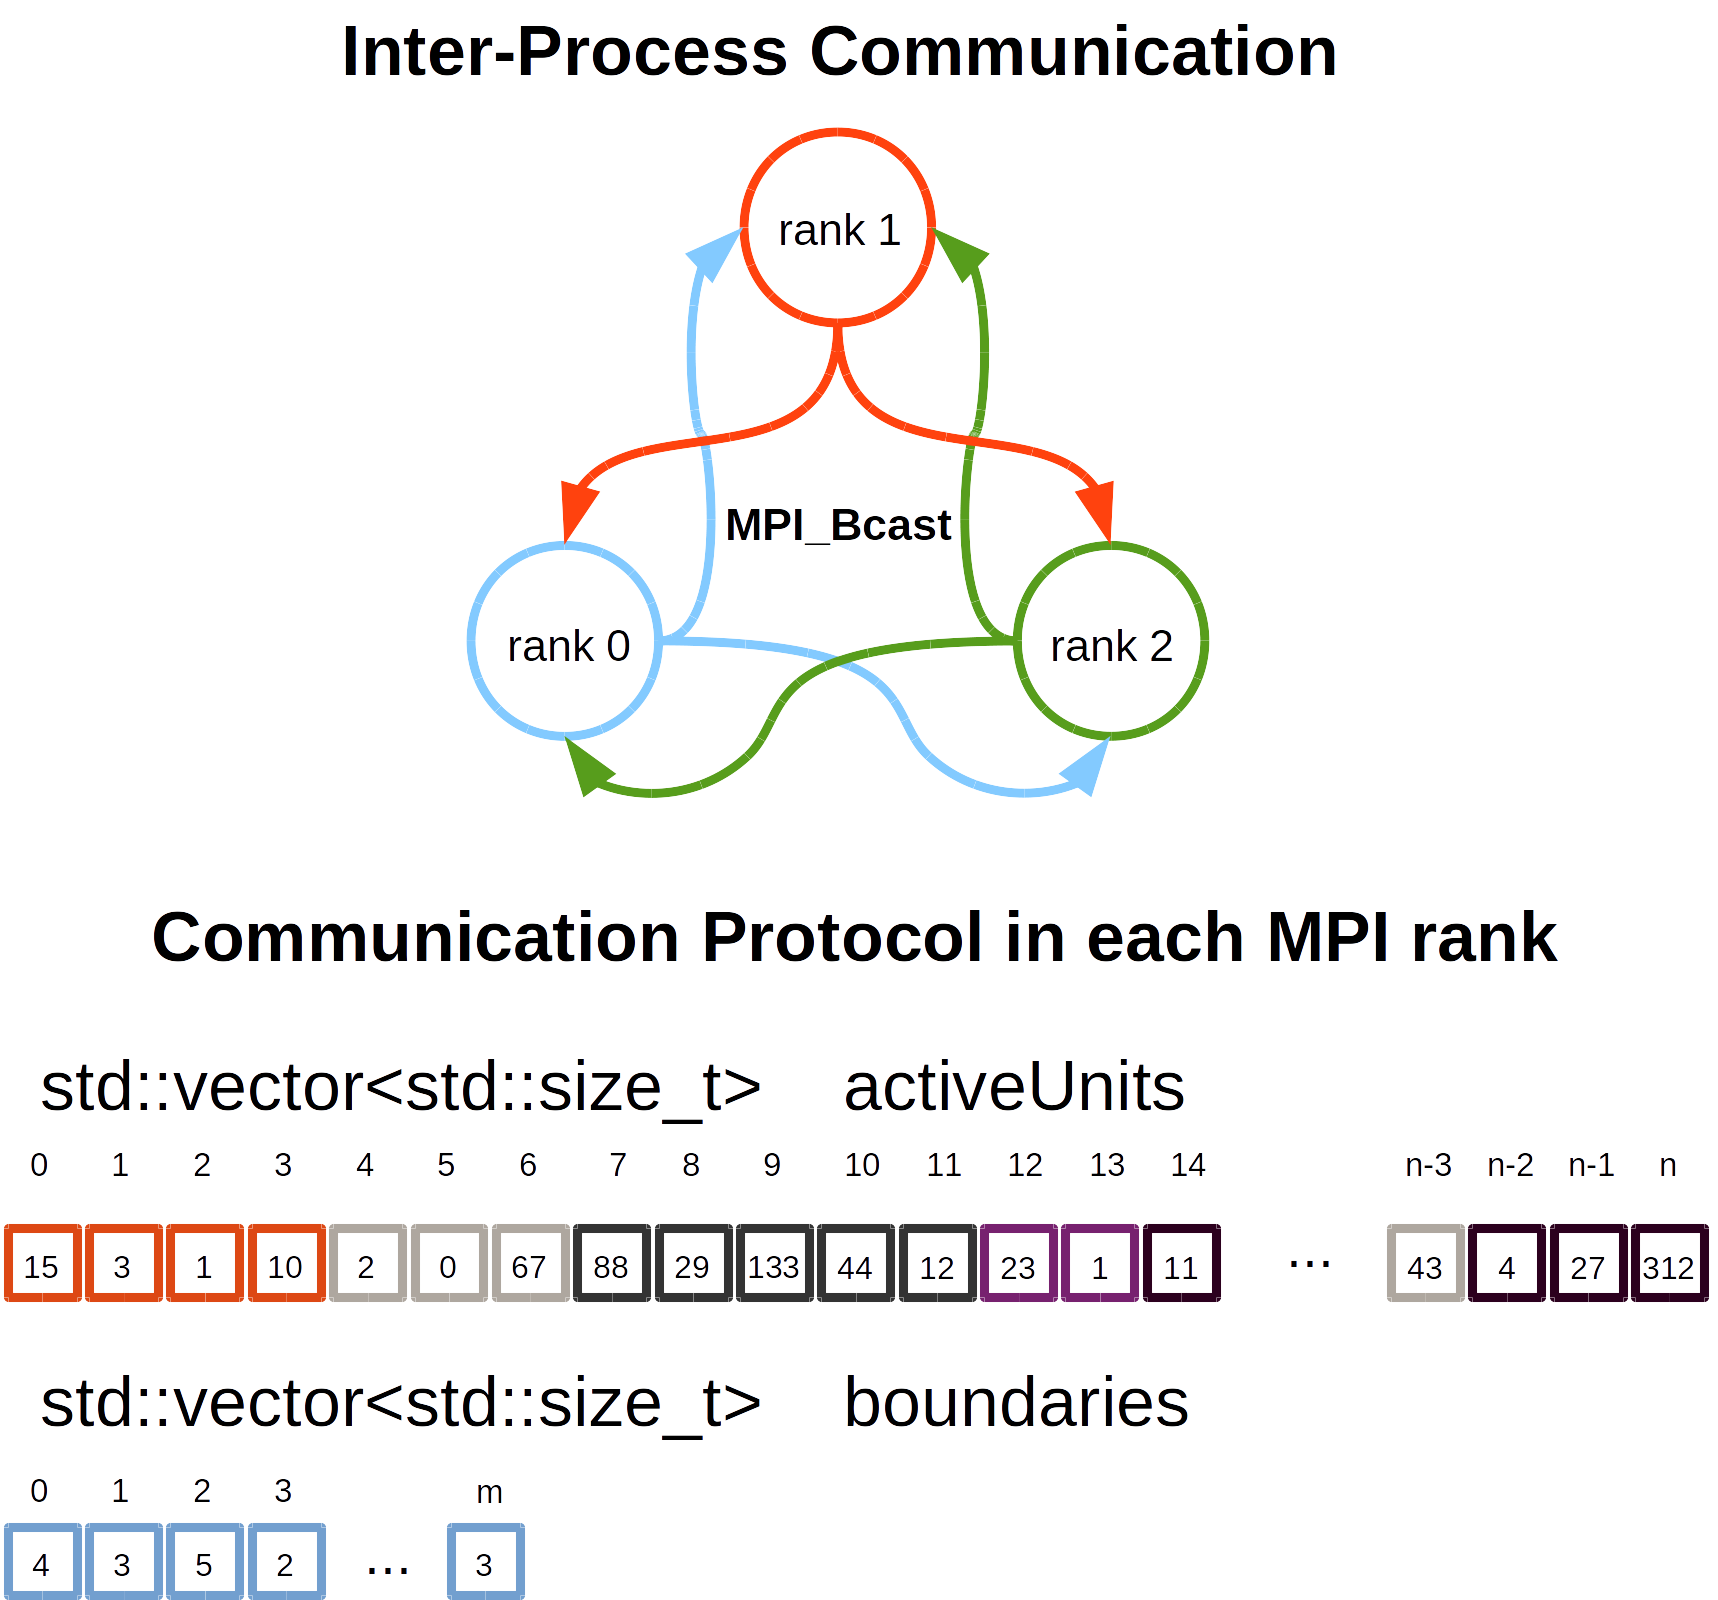
\includegraphics[width=0.7\textwidth]{BCast.png}
    \caption{\gls{ipc} entre diferentes procesos \gls{mpi}.}
    \label{fig:BCast}
\end{figure}

La \gls{el} usa sistemas I/O de archivo paralelos \gls{mpi} para guardar su estado en formatos Matlab/Octave.
Cada proceso \gls{mpi} agrupa tosos los datos correspondientes a sus \gls{csom_pl} en la \gls{el} y pone tales datos--formateados en Matlab/Octave--en una clase \texttt{std::stringstream}.
Luego, cada proceso \gls{mpi} comunica la parte del archivo que utilizará a los otros procesos \gls{mpi} para guardar los datos sin interferir con los otros procesos en el entorno \gls{mpi}.
Finalmente, cada proceso \gls{mpi} guarda todos sus datos con una única llamada a \gls{mpi} Write usando el \texttt{std::stringstream} completo.

La Fig.~\ref{fig:MPI_IO} muestra como cada proceso \gls{mpi} pone los datos formateados correspondientes a sus \gls{csom_pl} en una clase \gls{stl} \texttt{stringstream} template.
El proceso 0 también se hace cargo de la estructura, conectividad y parámetros de la \gls{el}.
Una vez que cada proceso tiene sus \texttt{stringstream} con los datos formateados, este comunica su cuota de archivo a los otros procesos.
Luego, cada proceso escribe su flujo de bytes en paralelo sin interferir con los otros procesos en el entorno \gls{mpi}.
Una \gls{el} con un número diferente de procesos puede cargar el mismo archivo sin afectar los resultados finales.
Cada proceso en la nueva \gls{el} carga el archivo completo en una clase \gls{stl} \texttt{stringstream} template y luego toma la información que le concierne desde tal estructura.

\begin{figure}[h!]
    \centering
    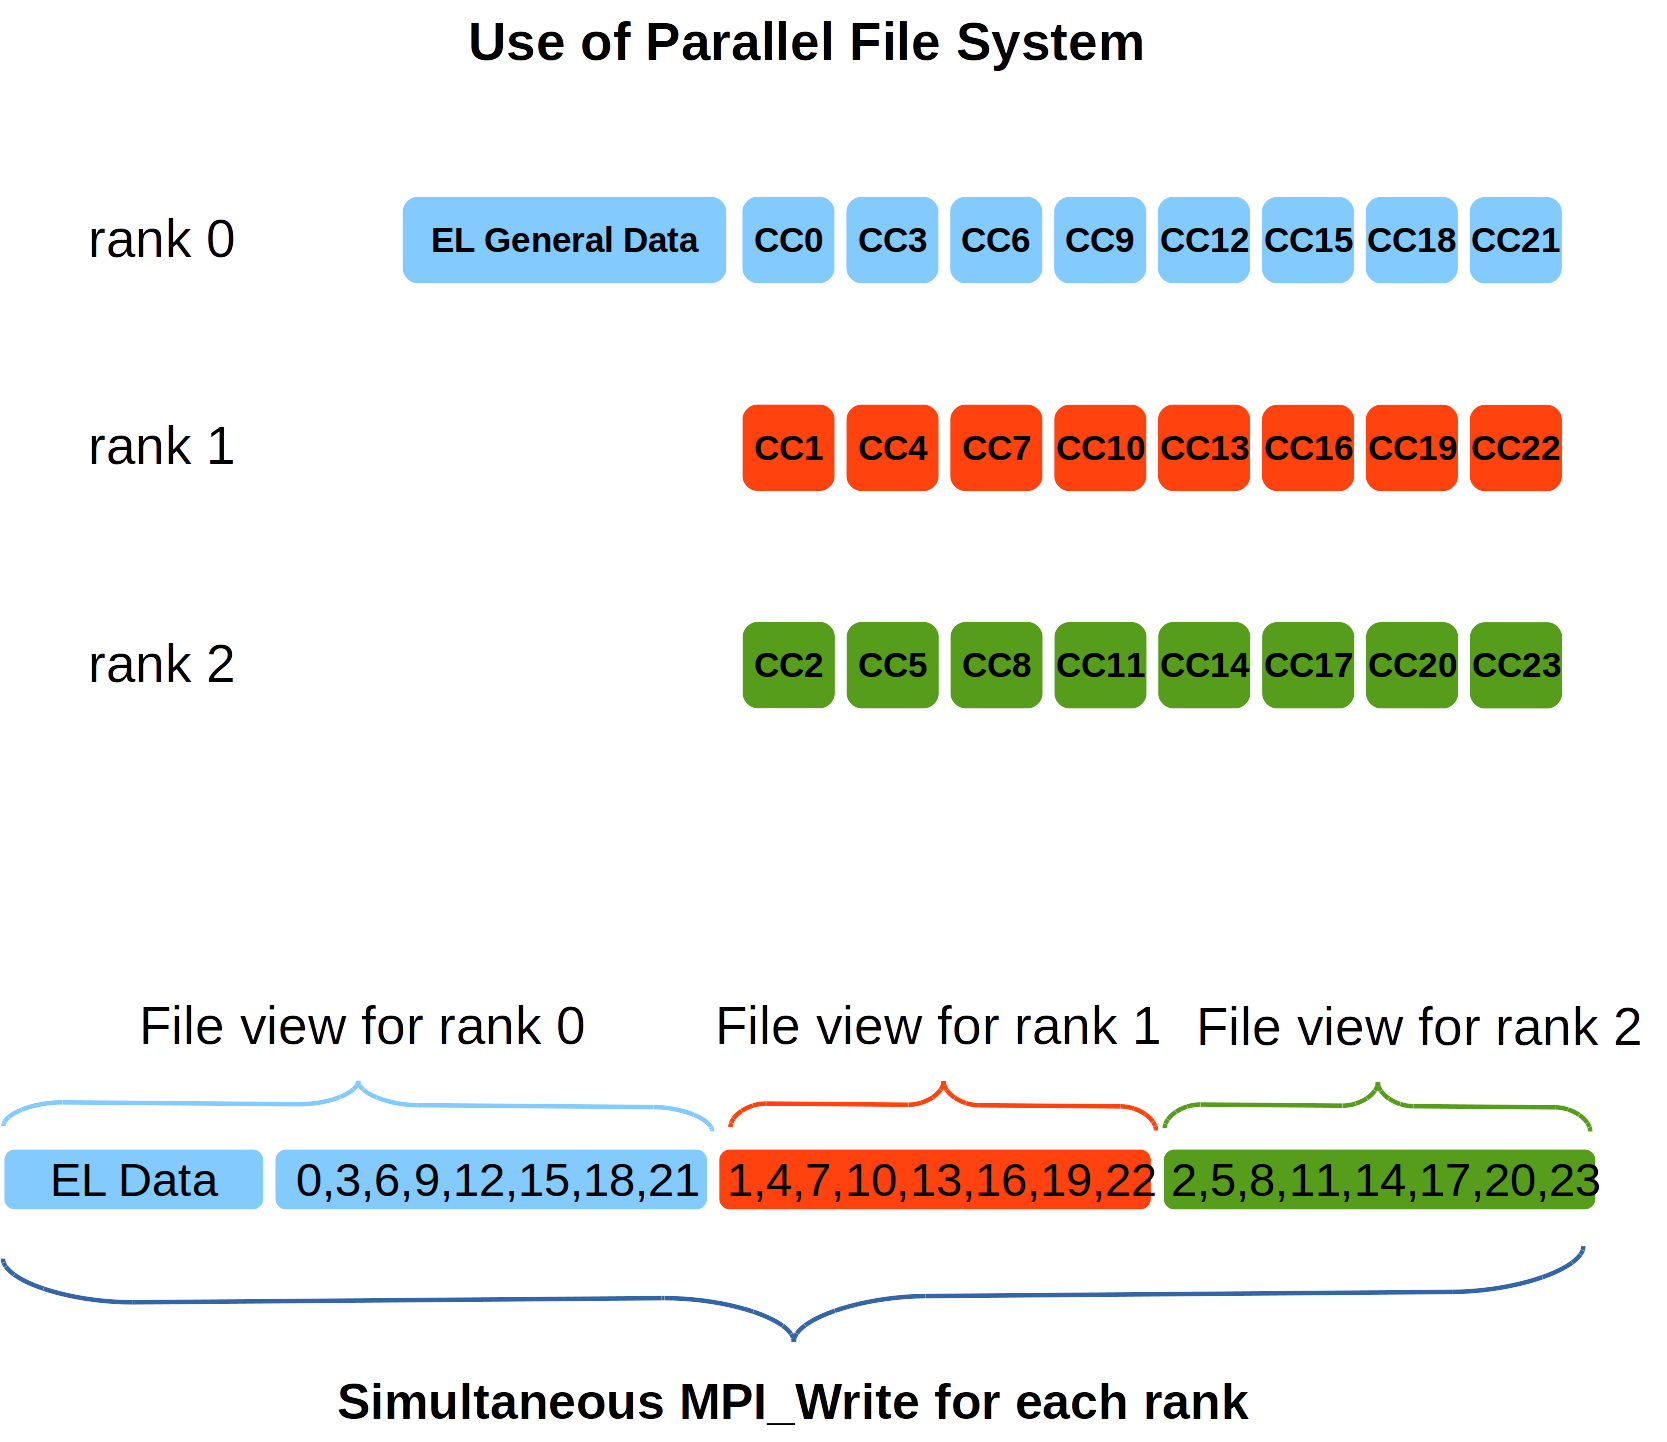
\includegraphics[width=0.7\textwidth]{MPI_IO.png}
    \caption{Distribución de la Información en la \gls{el} en un archivo para guardar su estado.}
    \label{fig:MPI_IO}
\end{figure}

En este trabajo, cada proceso \gls{mpi} corre en un nodo diferente y mantiene todos los datos que corresponden al objeto \gls{el}, tales como la dimensionalidad de la \gls{el}, los campos receptivos para cada \gls{cc}, los porcentajes de conexiones reales en cada campo receptivo para cada \gls{cc}, las dimensionalidades de las poblaciones para las \gls{cc_pl} así como la conectividad completa de cada \gls{cc} y todos los parámetros generales del modelo como las tasas de aprendizaje, las vecindades de aprendizaje, etc~\cite{10.1371/journal.pone.0217966}.
Aunque estos datos generales de la \gls{el} se replican en cada proceso \gls{mpi}, no son significativos comparados con los datos correspondientes a los objetos \gls{csom_pl}.
Cada proceso \gls{mpi} mantiene solo los datos de los \gls{csom_pl} que están a su cargo.
La Fig. \ref{fig:EL_ALG} muestra la organización general que sigue el algoritmo \gls{el}.

\begin{figure*}[ht]
    \centering
    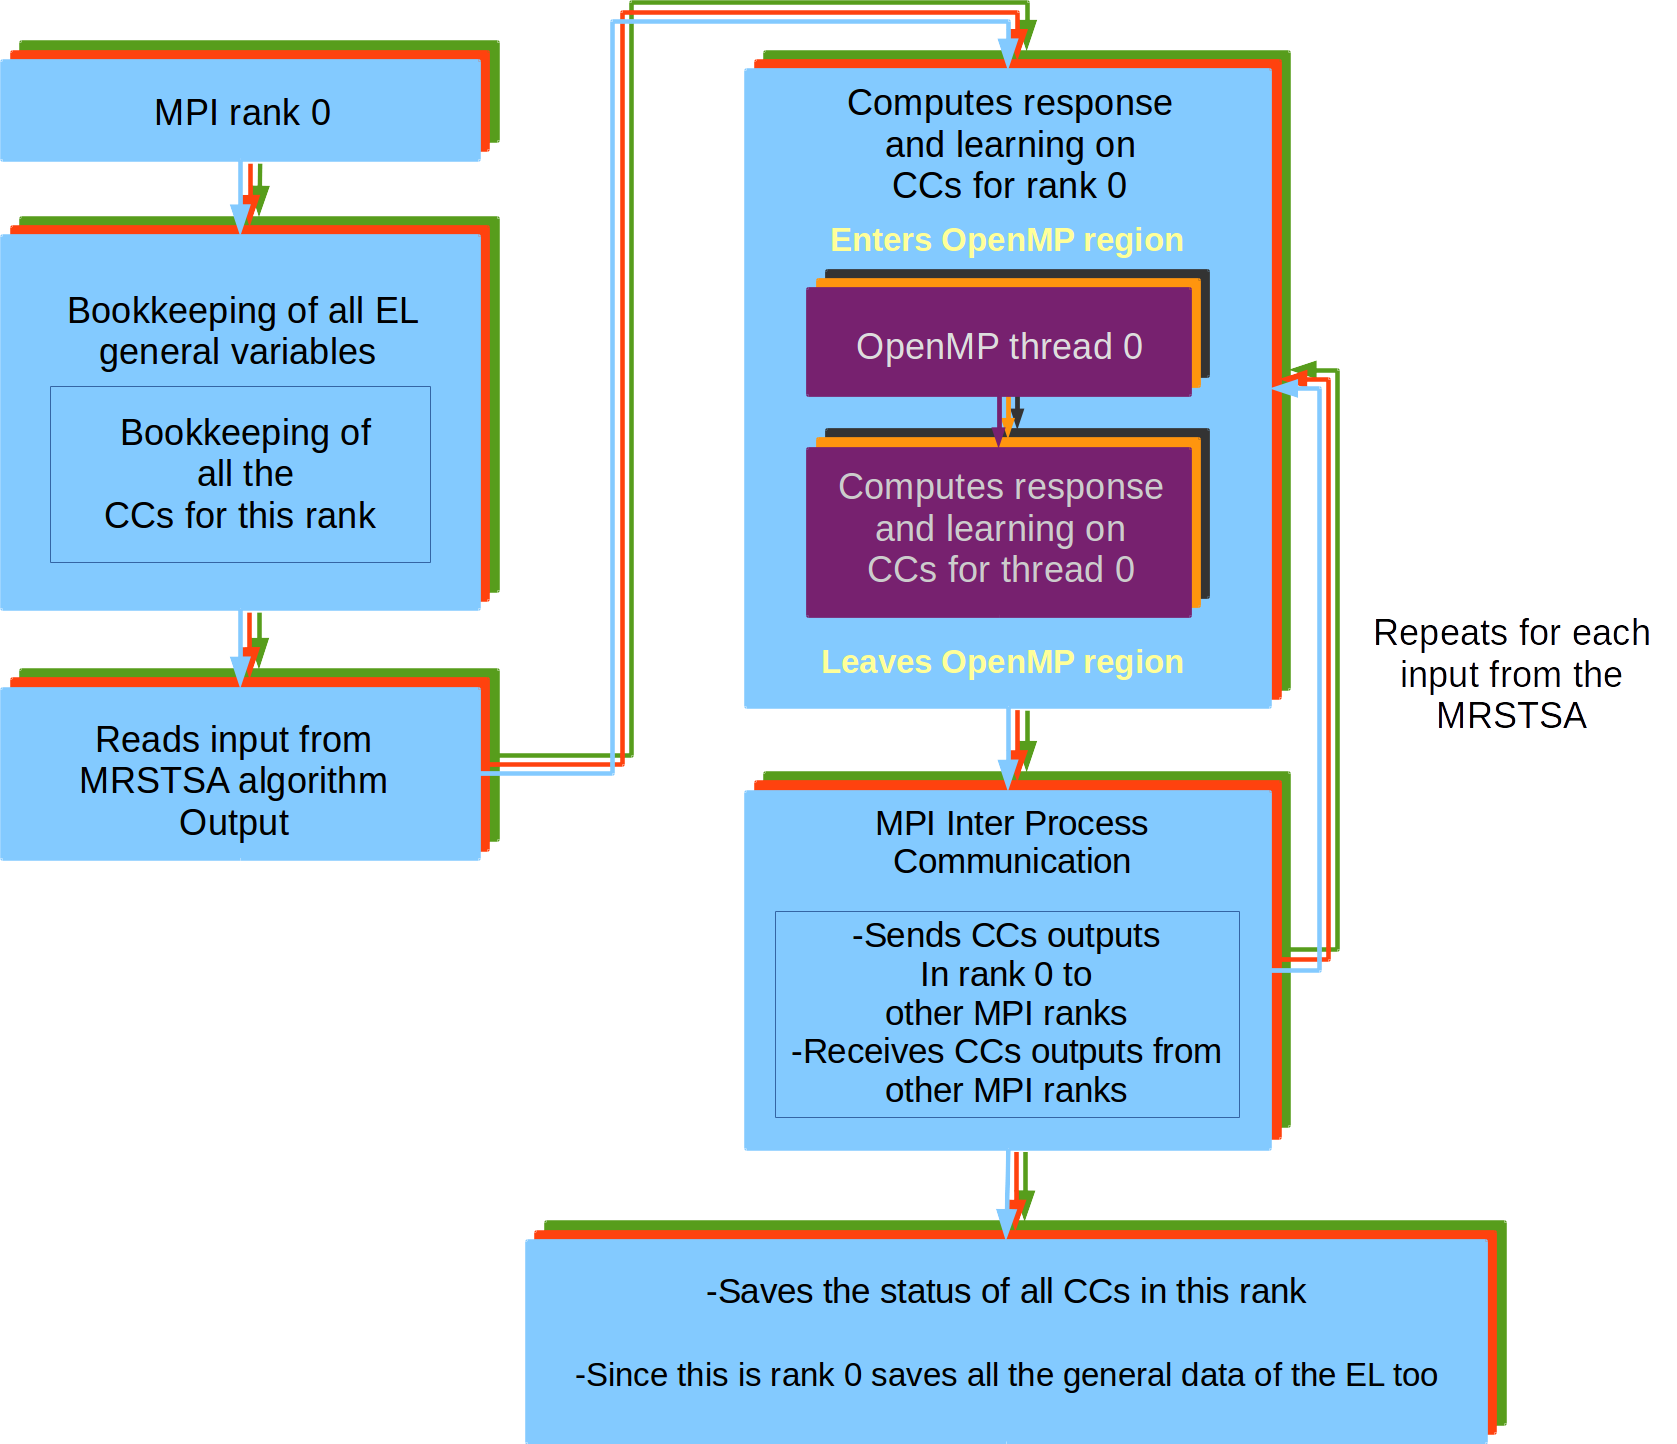
\includegraphics[width=0.7\textwidth]{EL_ALG.png}
    \caption{Organización general del algoritmo de la \gls{el}.} 
    \label{fig:EL_ALG}
\end{figure*}

En tal figura cada proceso \gls{mpi} mantiene una copia privada de la estructura entera de la \gls{el} pero solo mantiene los datos de los \gls{csom_pl} que le corresponden.
Cada proceso \gls{mpi} carga una copia privada de las entradas que vienen desde el algoritmo \gls{mrstsa}.
Luego cada proceso \gls{mpi} desarrolla la información de entrada por medio de las \gls{cc_pl} que están solamente a su cargo, primero entrando en la región \gls{omp} para distribuir las \gls{cc_pl} en un proceso entre los diferentes hilos \gls{omp} y luego dejando la región \gls{omp} y comunicando las salidas de todas las \gls{cc_pl} en la \gls{el} usando herramientas \gls{mpi} de \gls{ipc}.
Finalmente cada proceso \gls{mpi} guarda el estado de sus \gls{cc_pl} usando sentencias paralelas \gls{mpi}.
EL proceso \gls{mpi} 0 también guarda la estructura general de la \gls{el}.
}{
\subsection{\glsfirst{el} Parallel Implementation}
\label{EL_Parallelization}

The~\gls{el} simulates a patch of cortical tissue and incorporates columnar organization, spontaneous micro-columnar formation, partial \gls{nmda} depolarization and adaptation to contextual activations. We simulate pyramidal cells completely segregating proximal connections--from afferent dendritic branches--from distal connections--from lateral dendritic branches. This algorithm produces \glspl{sdr} that the brain uses to process information in all mammals, from mice to humans~\cite{barth_2012}.

We parallelized the \gls{el} by means of a hybrid \gls{mpi}+\gls{omp} paradigm distributing \glspl{csom} among \gls{mpi} ranks as a deck of cards is distributed among different players. Each \gls{mpi} rank ends up with one or more \glspl{csom} and the \glspl{csom} in each rank are distributed among different \gls{omp} threads.% (Fig. \ref{fig:Encoder_Parallelization}).% and Alg.~\ref{ccs_distribution}).

Fig.~\ref{fig:Encoder_Parallelization} shows the distribution of \gls{csom} objects in an \gls{el} with 3 by 8 (24) \glspl{cc} among three \gls{mpi} ranks with three \gls{omp} threads per rank. Certain ranks could take care of a different number of \glspl{csom} depending on the number of \gls{mpi} ranks as well as the number of \glspl{cc} in the \gls{el}. Each \gls{mpi} rank distributes its \glspl{csom} among different threads in the same fashion.

\begin{figure}[h!]
    \centering
    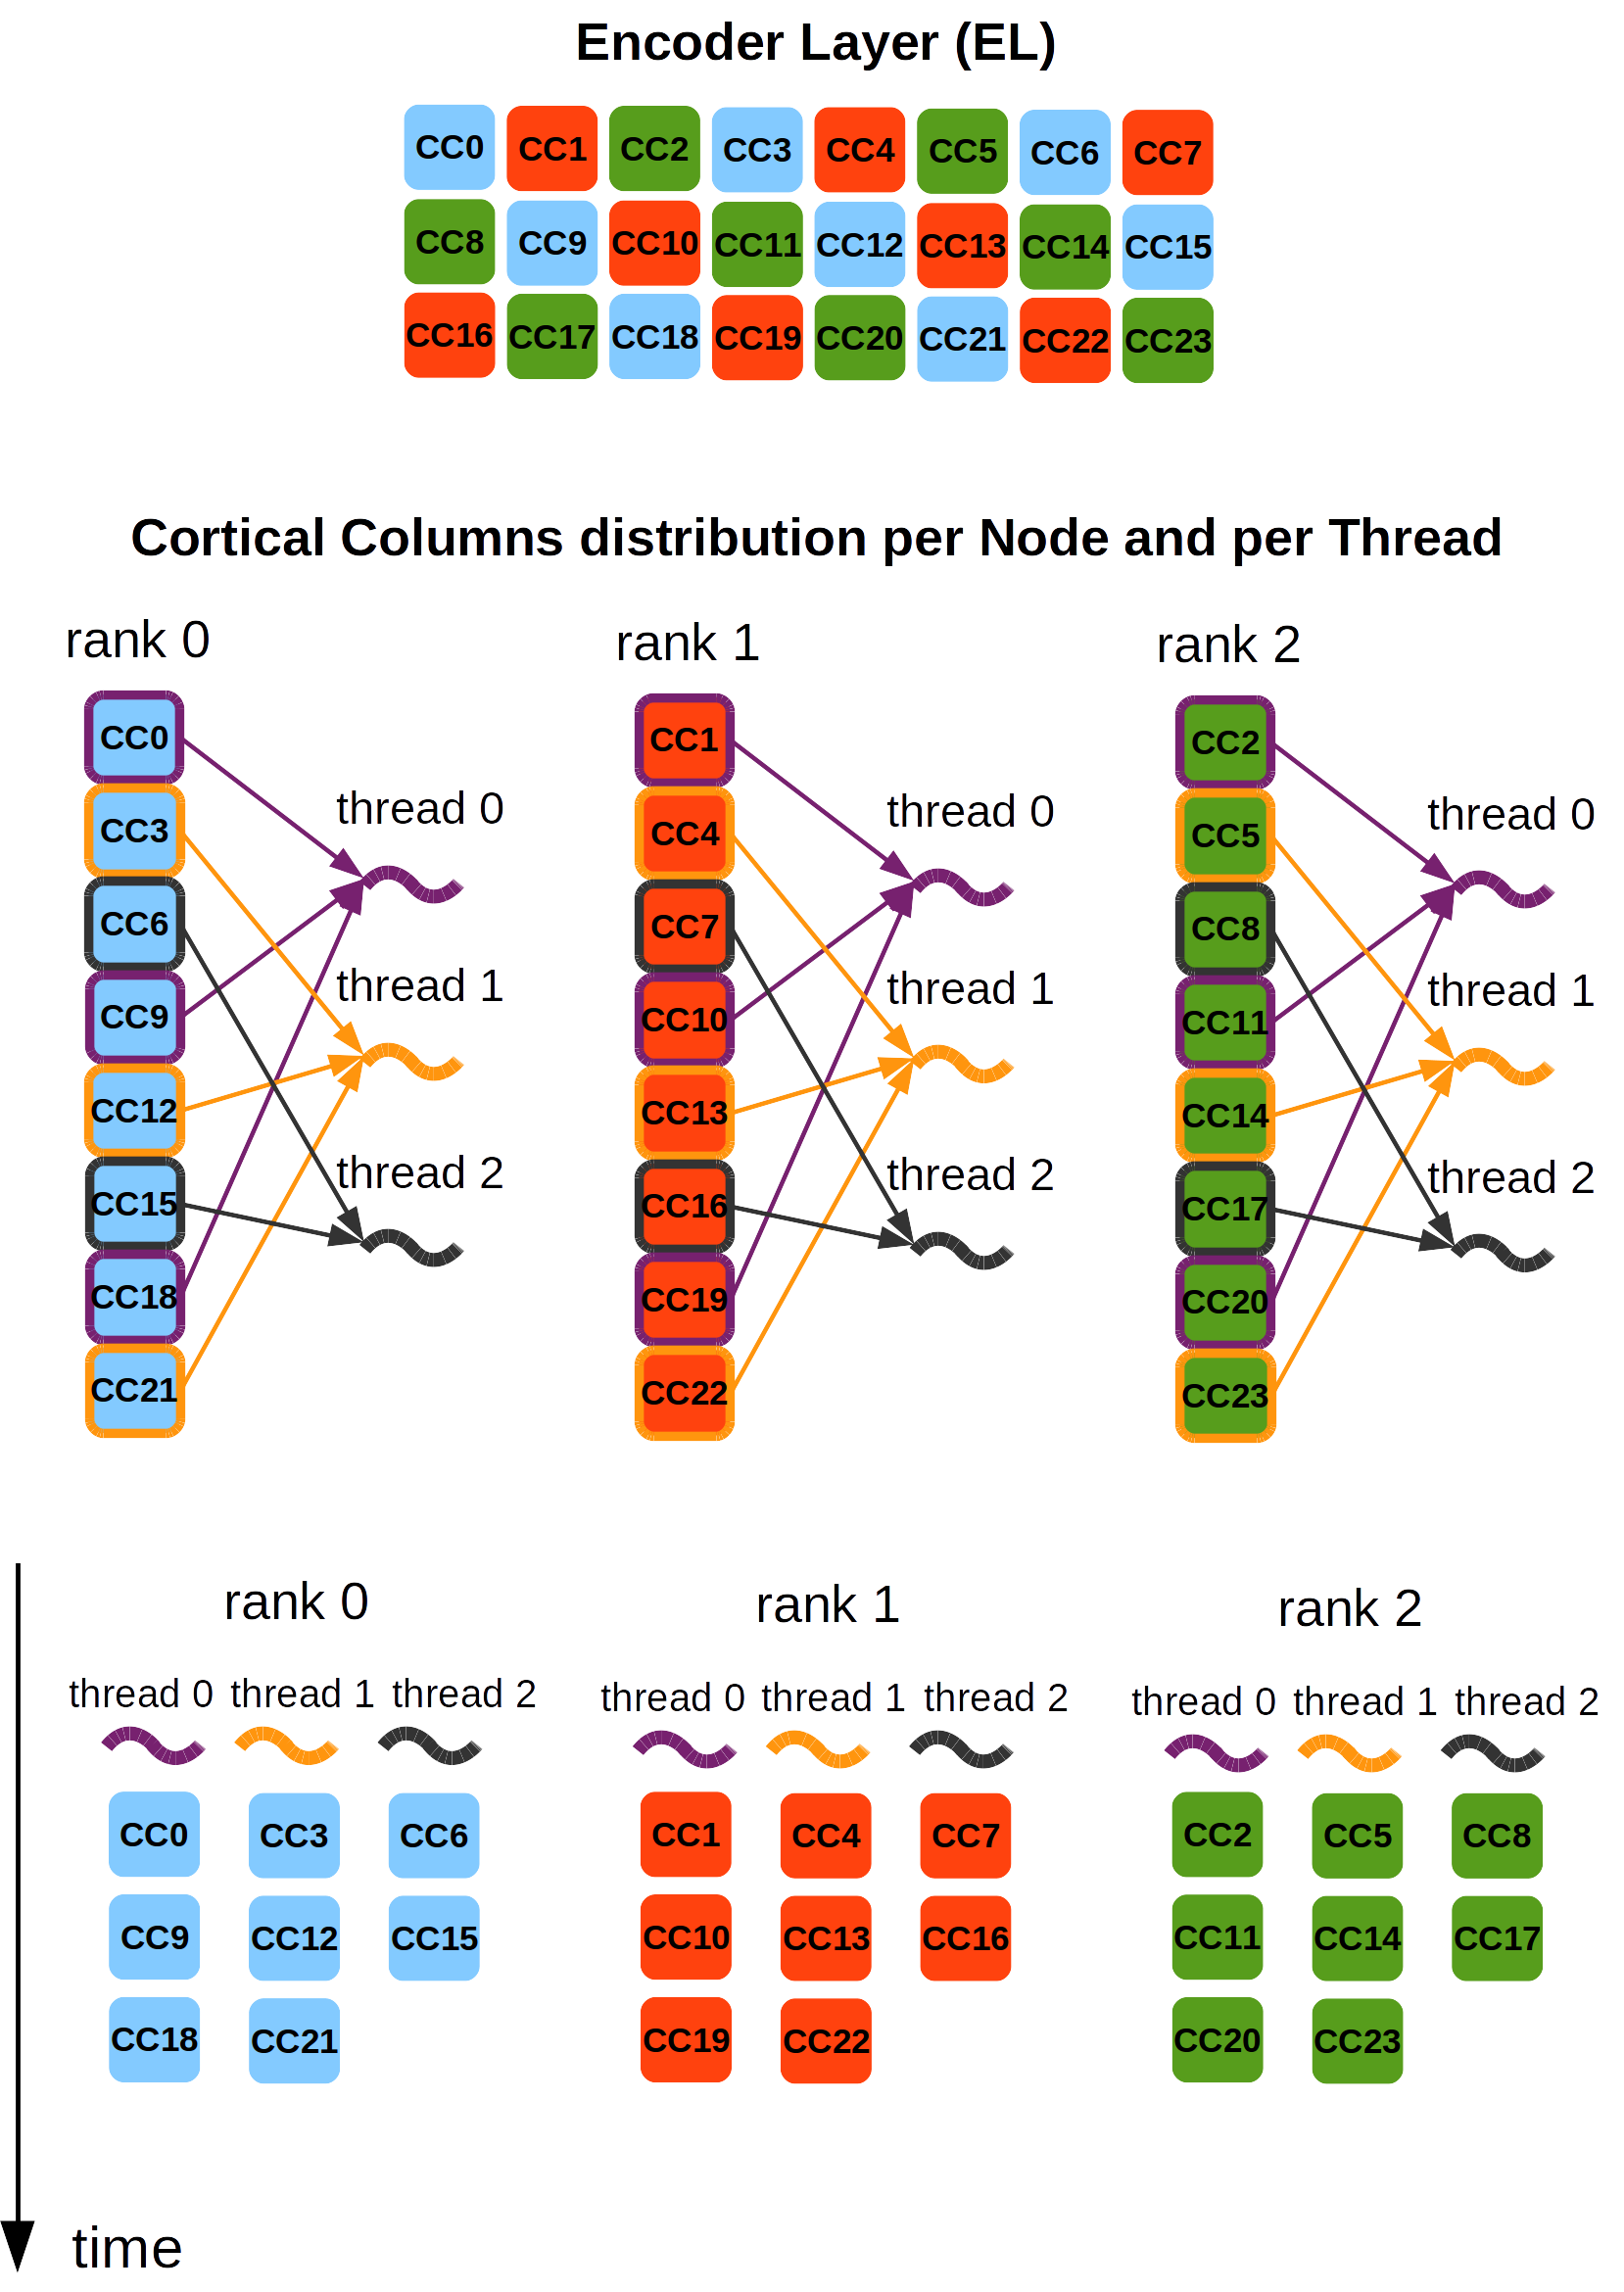
\includegraphics[width=0.9\textwidth]{Encoder_Parallelization.png}
    \caption{\glsfirst{el} \gls{mpi}+\gls{omp} parallelization.}
    \label{fig:Encoder_Parallelization}
\end{figure}

Information among \gls{mpi} ranks must be transferred in each time step. Basically all the information needed by each process is the identity of the active neural units in each \gls{cc} of the \gls{el}. We gather all the information corresponding to the \glspl{csom} in each rank and then use \gls{mpi} Bcast function to transmit such information using a special communication protocol by means of which we specify the boundaries in the information corresponding to each \gls{csom}. By means of this strategy each \gls{mpi} rank has to call \gls{mpi} Bcast just once in order to transmit its data.

Fig. \ref{fig:BCast} shows that \gls{ipc} is carried out at each time step since each \gls{mpi} rank requires the complete \gls{el} output at each time step. Each \gls{mpi} rank broadcasts the information corresponding to its \glspl{cc} to the other ranks in the \gls{mpi} environment. In the communication protocol to transmit information among \gls{mpi} ranks in the \gls{el} all the information is transmitted in two \gls{stl} vectors--\texttt{activeUnits} and \texttt{boundaries}. The vector \texttt{activeUnits} identifies the active neural units in the \glspl{cc} inside a \gls{mpi} rank and \texttt{boundaries} identifies the number of active units that belong to the different \glspl{cc}. The figure shows $n+1$ active units in the \glspl{cc} managed by certain \gls{mpi} rank and $m+1$ \glspl{cc} managed by such \gls{mpi} rank.

\begin{figure}[h!]
    \centering
    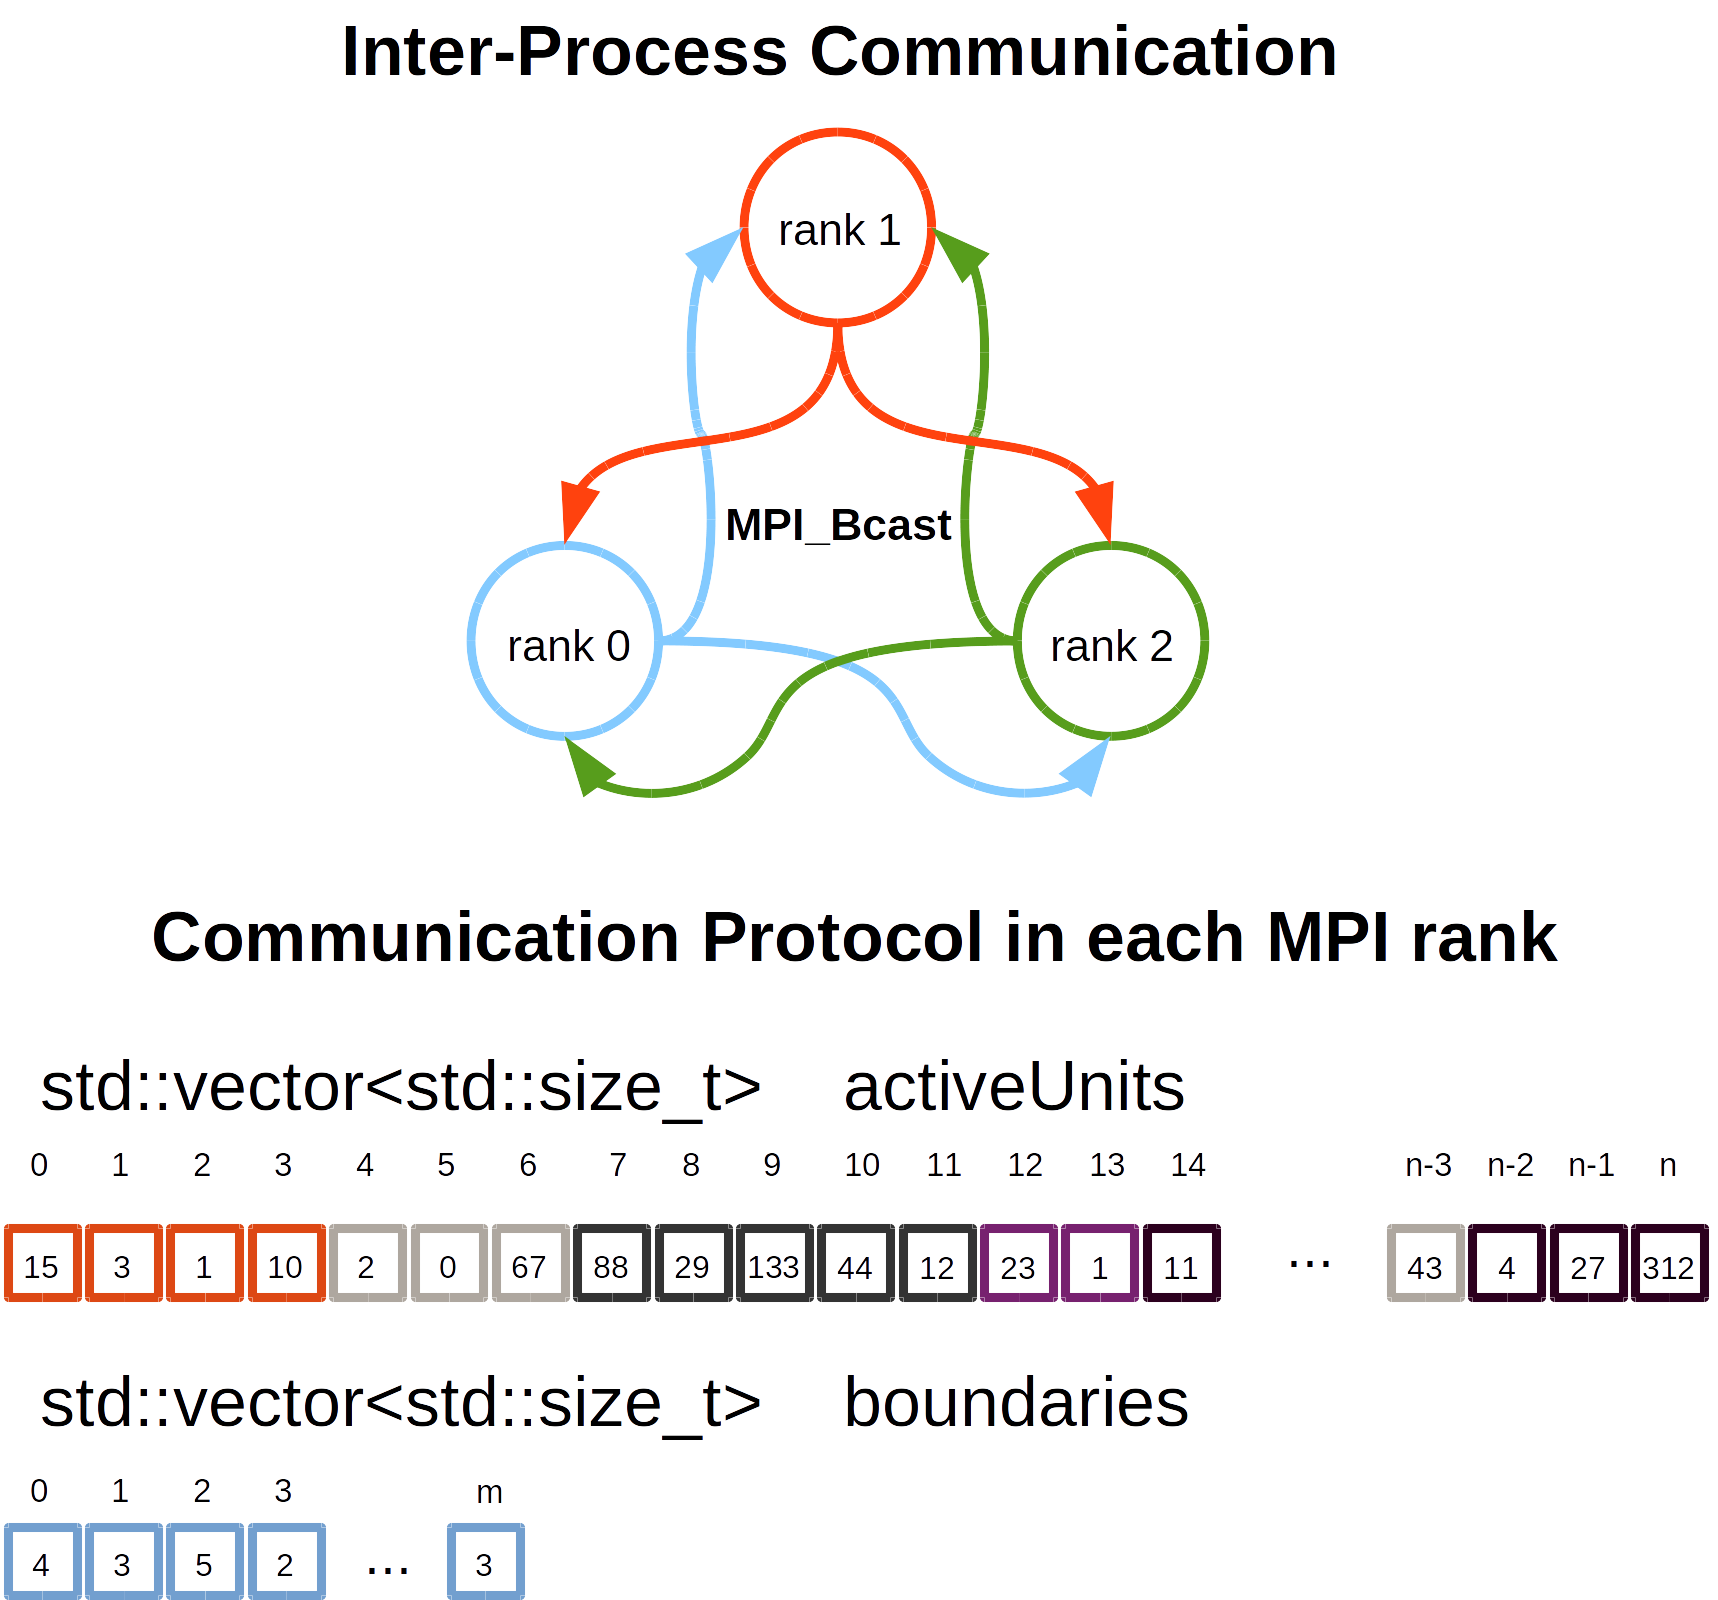
\includegraphics[width=0.9\textwidth]{BCast.png}
    \caption{\gls{mpi} \gls{ipc} among different ranks.}
    \label{fig:BCast}
\end{figure}

The \gls{el} uses \gls{mpi} I/O parallel file system to save its status in Matlab/Octave format. Each \gls{mpi} rank gathers all the data corresponding to its \glspl{csom} in the \gls{el} and puts such data--formatted in Matlab/Octave--in a \texttt{std::stringstream} class. Then such \gls{mpi} rank communicates the part of the file it will use to the other \gls{mpi} ranks in order to store the data without interfering with the other ranks in the \gls{mpi} environment. Finally, each \gls{mpi} rank saves all its data with a unique call to \gls{mpi} Write using the complete \texttt{std::stringstream}.

Fig.~\ref{fig:MPI_IO} shows how each \gls{mpi} rank puts the formated data corresponding to its \glspl{csom} in a \gls{stl} \texttt{stringstream} class template. Rank 0 also takes care of the \gls{el} structure, connectivity and parameters. Once each rank has its \texttt{stringstream} with the formated data, it communicates its file view to the other ranks. Then each rank writes its stream of bytes in parallel without interfering with other ranks in the \gls{mpi} environment. An \gls{el} with a different number of ranks can load the same file without affecting the final results. Each rank in the new \gls{el} loads the complete file in a \gls{stl} \texttt{stringstream} class template and then takes the informations that concern it from such structure.

\begin{figure}[h!]
    \centering
    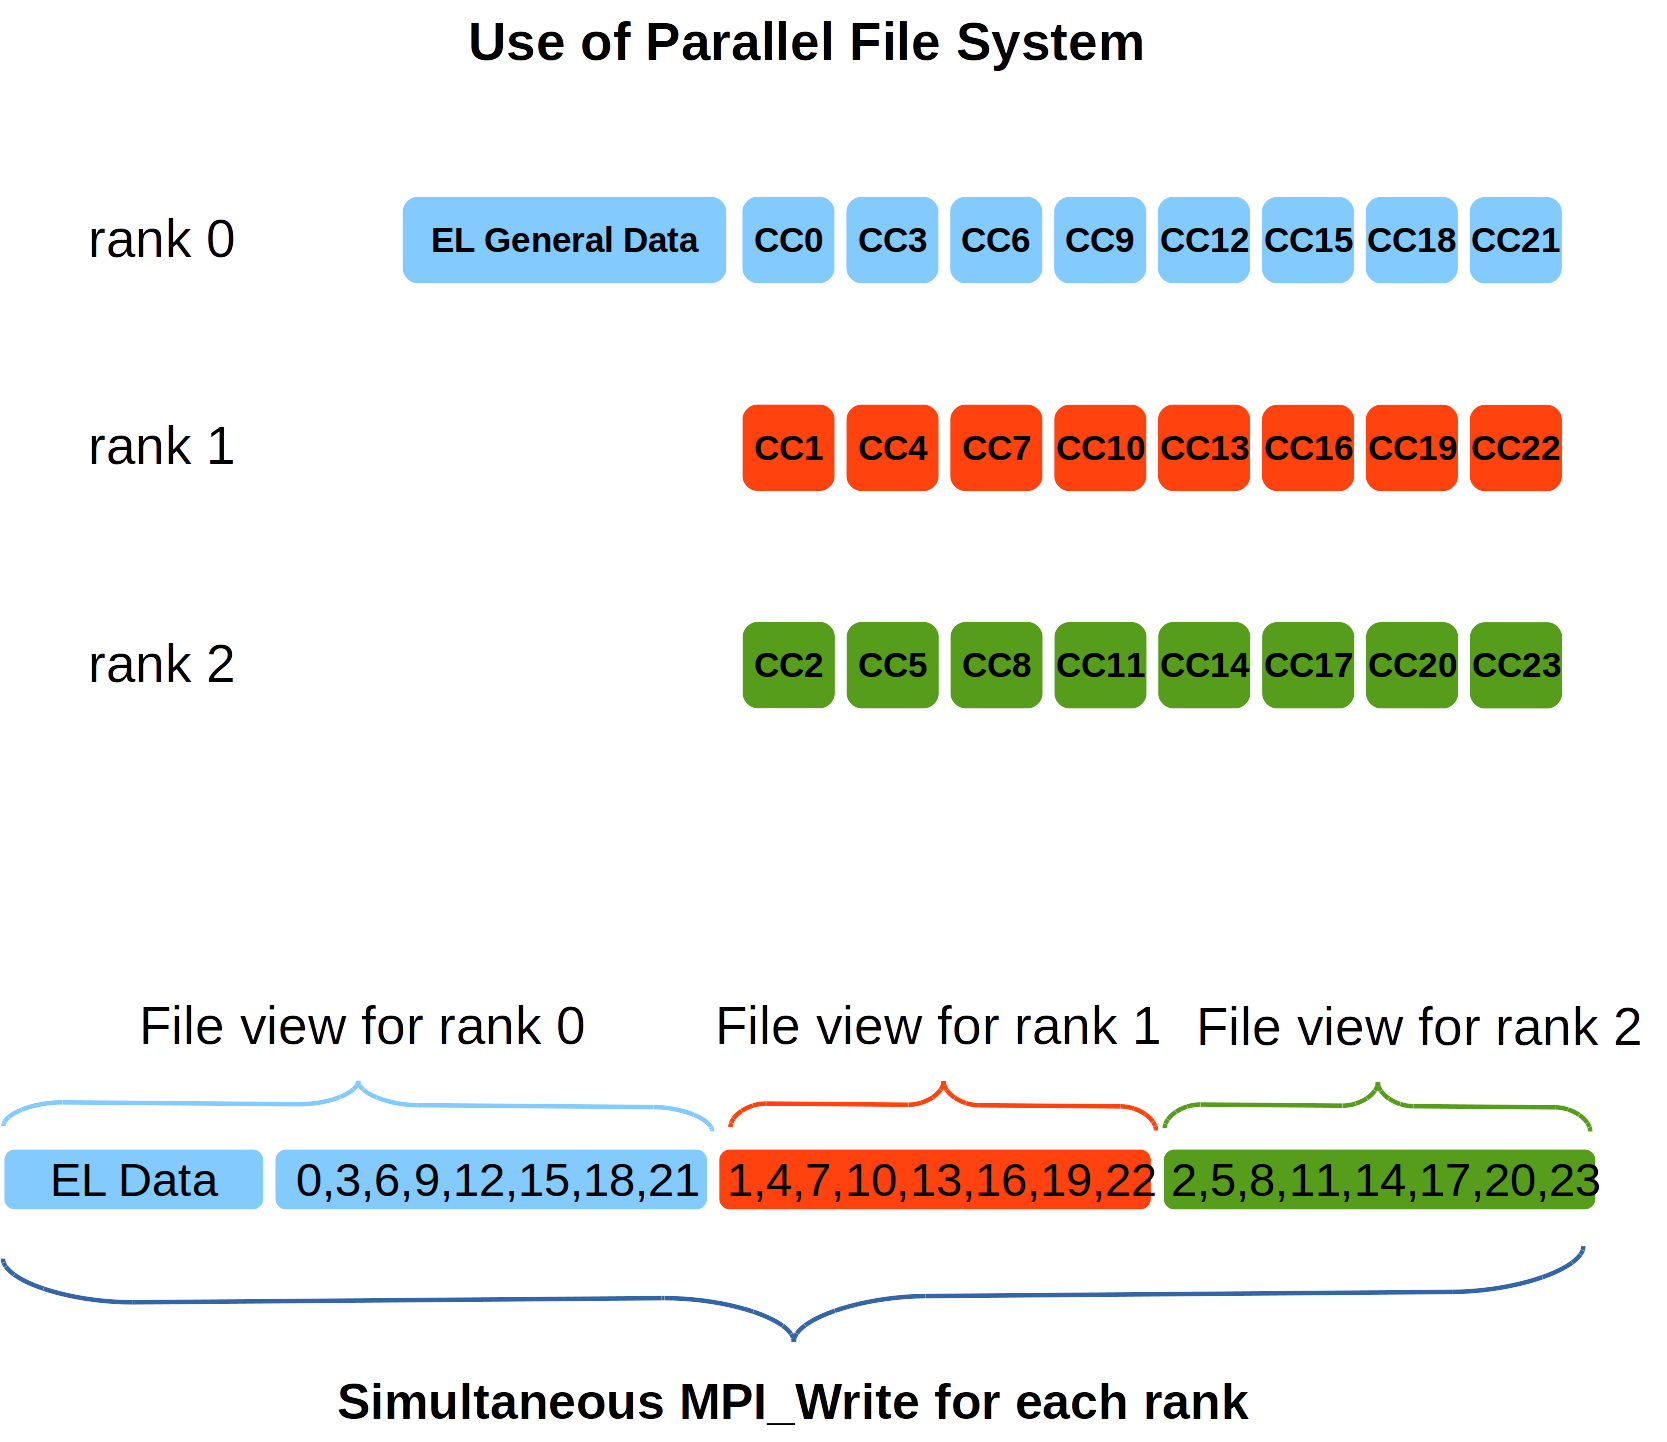
\includegraphics[width=0.9\textwidth]{MPI_IO.png}
    \caption{\gls{el} information distribution in a file to save its status.}
    \label{fig:MPI_IO}
\end{figure}

In this work, each \gls{mpi} rank runs in a different node and keeps all the data that corresponds to the \gls{el} object, such as \gls{el} dimensionality, receptive fields for each \gls{cc}, percentages of real connections in each receptive field for each \gls{cc}, population dimensionalities for the \glspl{cc} as well as the complete connectivity of each \gls{cc} and all the general parameters of the model such as learning rates, learning neighborhoods, etc~\cite{10.1371/journal.pone.0217966}. Although this general \gls{el} data is replicated in each \gls{mpi} rank, this is not significant compared to the data corresponding to the \glspl{csom} objects. Each \gls{mpi} rank keeps only the data for those \glspl{csom} which are under its charge. Fig. \ref{fig:EL_ALG} depicts the general layout that follows the \gls{el} algorithm.

\begin{figure*}[ht]
    \centering
    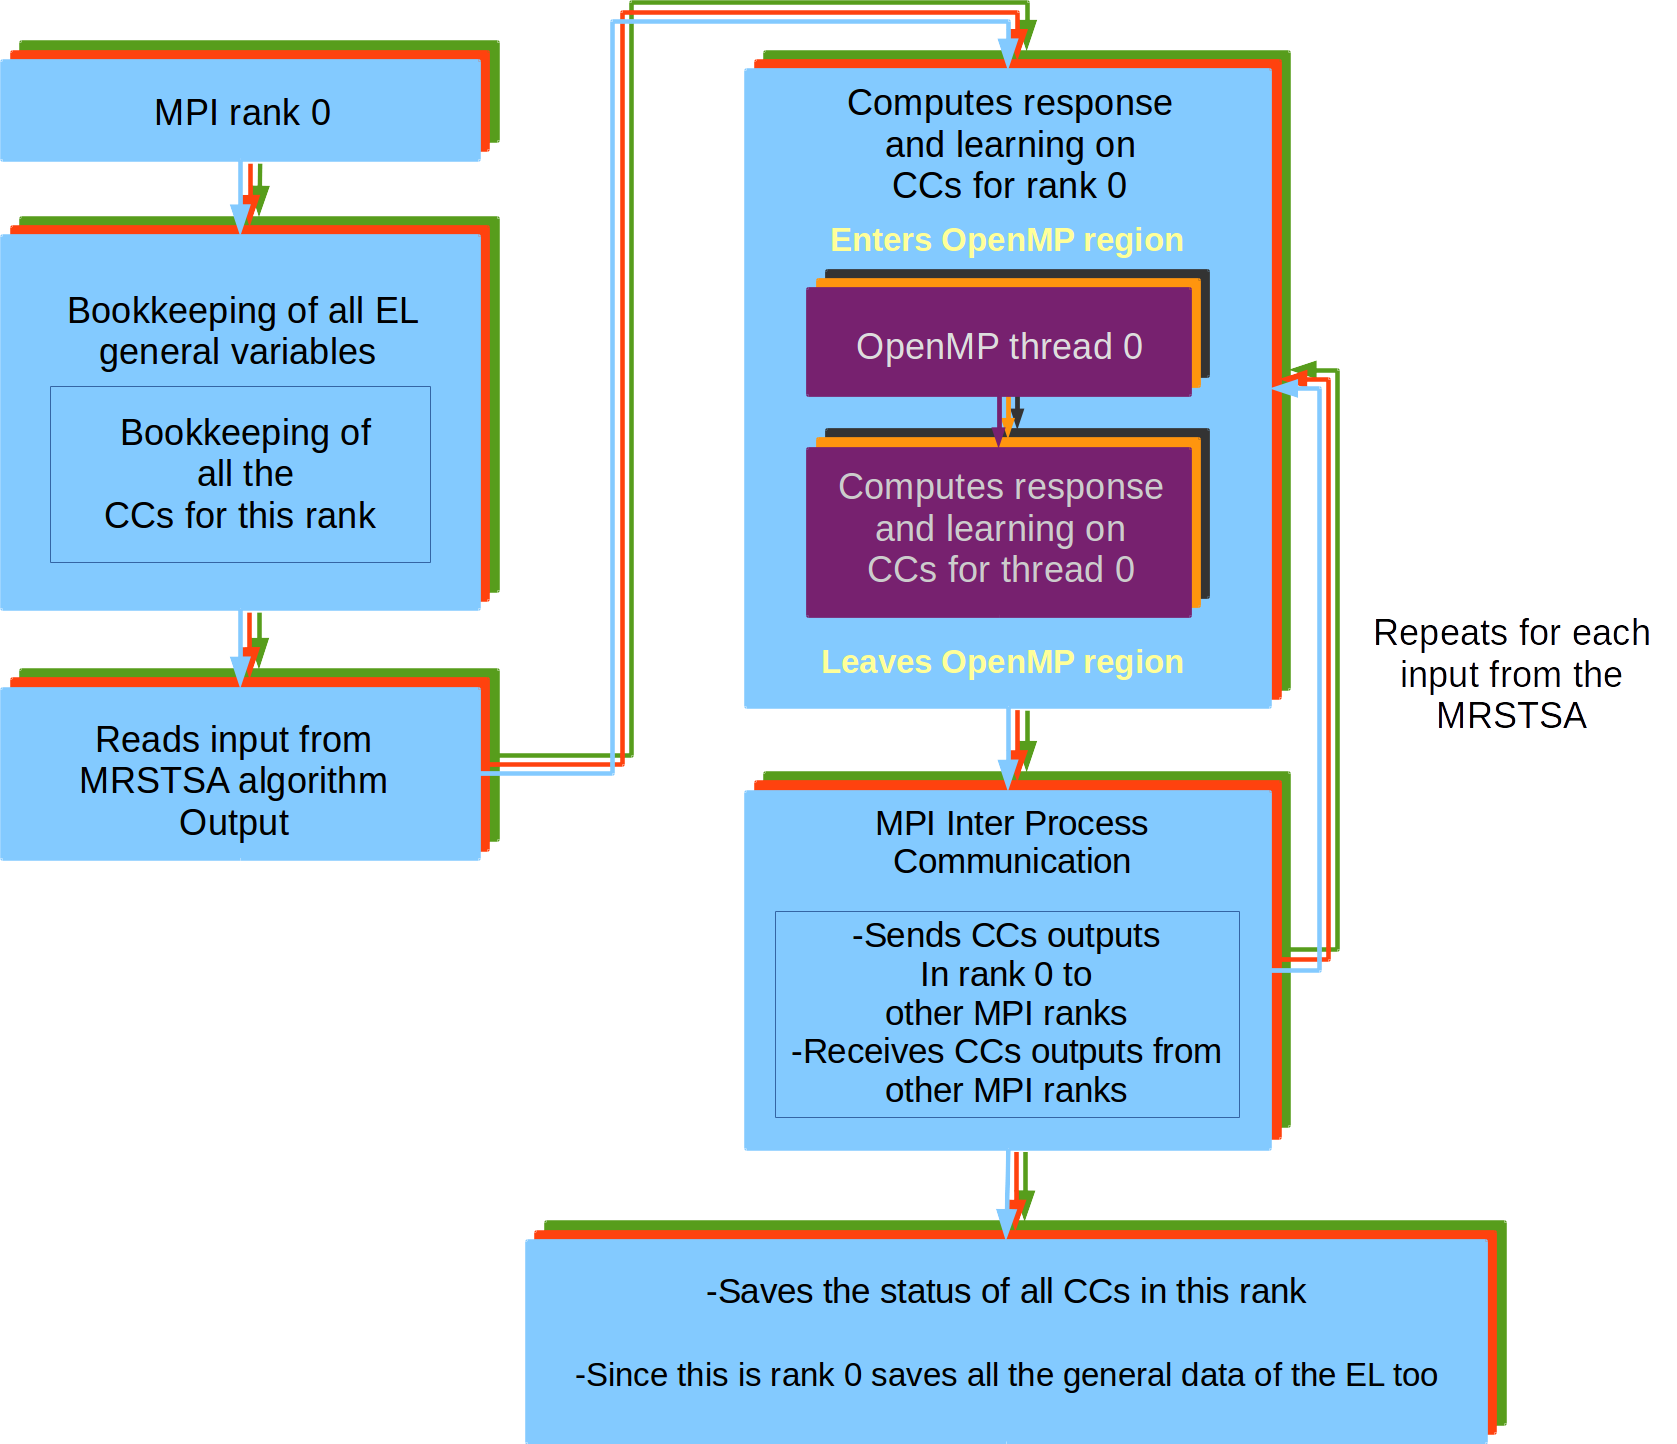
\includegraphics[width=0.9\textwidth]{EL_ALG.png}
    \caption{General layout of the \gls{el} algorithm.} 
    \label{fig:EL_ALG}
\end{figure*}

In such figure each \gls{mpi} rank keeps a private copy of the entire \gls{el} structure but only keeps the data of the \glspl{csom} which corresponds to it. Each \gls{mpi} rank loads a private copy of the inputs that come from the \gls{mrstsa} algorithm. Then each \gls{mpi} rank processes the input information by means of only the \glspl{cc} which are under its charge, first entering to an \gls{omp} region in order to distribute \glspl{cc} in the rank among different \gls{omp} threads and then leaving the \gls{omp} region and communicating the outputs of all \glspl{cc} in the \gls{el} using \gls{mpi} \gls{ipc} tools. Finally each \gls{mpi} rank saves the status of its \glspl{cc} using \gls{mpi} parallel I/O sentences. \gls{mpi} rank 0 also saves the general structure of the \gls{el}.
}

















\iftoggle{DEBUG}{
\section{Resultados}

En este trabajo probamos la eficiencia en escalabilidad de las estrategias de paralelización usadas en el \gls{cstm} por medio de pruebas de escalado fuertre y débil (\emph{strong and weak scaling tests}).
Realizamos nuestras pruebas en Cooley, un cluster para analizar y visualizar datos producidos en supercomputadoras de alto desempeño en el Laboratorio Nacional Argonne.
Cooley tiene 126 nodos de computación; cada nodo cuenta con 12 núcleos \gls{cpu} y una targeta \gls{gpu}-dual NVIDIA Tesla K80.
El desempeño agregado pico \gls{gpu} está sobre los 293 teraflops en doble precisión (usando los relojes \gls{gpu} base), y el sistema completo tiene un total de 47 terabytes de RAM de sistema y 3 terabytes de RAM \gls{gpu}.
El acceso a Cooley se provee por medio de dos nodos login, los que proveen capacidades de envío de trabajos y compilación.
La planificación es provista por el planificador de trabajos Cobalt.

La configuración del nodo de Cooley cuenta con arquitectura Intel Haswell con dos procesadores Intel Haswell E5-2620 v3 de 2.4 GHz (6 núcleos por \gls{cpu}, un total de 12 núcleos), una NVIDIA Tesla K80 (con dos \gls{gpu_pl}), 384GB de RAM, 24 GB de GPU RAM (12 GB por GPU), interconexión FDR Infiniband y 345GB de espacio local de borrador.

El \emph{\gls{alcf}} utiliza SoftEnv para manejar el entorno.
Un archivo llamado .soft.cooley en el directorio \texttt{home} es creado para tal propósito.
El compilador GNU versión 7.1.0 está instalado y se hace disponible agregando \texttt{+gcc-7.1.0} a .soft.cooley.
Múltiples versiones de \gls{mpi} se encuentran disponibles, controladas por el archivo .soft.cooley.
La asignación provee MPICH2 para utilizar con el compilador GNU.
Agregamos la línea \texttt{+mvapich2-2.2} al archivo .soft.cooley para tal fin.

También agregamos \texttt{+matlab} para utilizar matlab versión 8.6.0.267246 (R2015b), \texttt{+anaconda3-4.0.0} para usar Anaconda 4.0.0 para Python 3 - con actualizaciones de NumPy, SciPy, etc y \texttt{+ddt} para usar Allinea DDT Debugger version 18.2.1.
Usamos Malab para pre-procesar las salidas del modelo a los fines de preparar los datos para la clasificación con \gls{svm} usando \emph{\gls{libsvm}} sobre Matlab.
Finalmente utilizamos el paquete Anaconda para el algoritmo de Generación de Corpus con los paquetes Numpy y \texttt{mpi4py}.

Para compilar nuestro código utilizamos GCC 7.1.0 con las siguientes banderas: \texttt{-O3 -mcmodel=large -fopenmp -Wall -pedantic -std=c++14}.

El uso del comando \texttt{qsub} permite al usuario entregar trabajos; la entrega debe ser por medio de un script que será ejecutado en el nodo rank0 asignado al usuario por el planificador.
El script tendrá acceso a una variable de entorno denominada \texttt{COBALT\_NODEFILE}, que es el nombre de un archivo preparado para usar con la opción \texttt{mpiexec -f}. 
El número de procesos \gls{mpi} que corren por trabajo depende completamente de los argumentos suministrados a \texttt{mpiexec} en el script.

Como mínimo, a \texttt{qsub} se le debe proveer con el número de nodos deseados (\texttt{-n}), el tiempo asignado para el trabajo (\texttt{-t}) y la ruta al script.
Si el ususario está asociado con más de un proyecto, el nombre del proyecto debe ser provisto utilizando la opción \texttt{-A}.
Como ejemplo de un envío de trabajo utilizamos \texttt{qsub -n 9 -t 240 -A neurophon ./test\_ERRLayer9.sh} donde pedimos por 9 nodos durante 4 horas para hacer inferencia con nuestro modelo.

Corrimos el modelo usando mpiexec versión 3.1.4 con las siguientes opciones: \texttt{mpiexec -n} el número de procesos \gls{mpi} a ser usados \texttt{-f \$COBALT\_NODEFILE -env MV2\_ENABLE\_AFFINITY=0 -ppn 1 ./Test} los argumentos del programa.
Con tales opciones corrimos un proceso \gls{mpi} por nodo y distribuimos un puñado de hilos \gls{omp} para utilizar las \gls{cpu_pl} en cada nodo.
Definimos el número de hilos dentro del código en las sentencias pragma: \texttt{\#pragma omp parallel for default(none) shared(...) num\_threads(9)}.
}{
\section{Results}

In this paper we tested the scalability efficiency of the parallelization strategies used in the~\gls{cstm} by means of \emph{strong} and \emph{weak} scaling tests. We conducted our tests on Cooley, a cluster to analyze and visualize data produced on high-end supercomputers at Argonne National Laboratory. Cooley has 126 compute nodes; each node has 12 CPU cores and one NVIDIA Tesla K80 dual-GPU card. Aggregate GPU peak performance is over 293 teraflops double precision (using base GPU clocks), and the entire system has a total of 47 terabytes of system RAM and 3 terabytes of GPU RAM. Access to Cooley is provided by two login nodes, which provide compilation and job submission capabilities. Job scheduling is provided by the Cobalt job scheduler.

The Cooley node configuration has an Intel Haswell architecture with two 2.4 GHz Intel Haswell E5-2620 v3 processors (6 cores per CPU, 12 cores total), one NVIDIA Tesla K80 (with two GPUs), 384GB RAM, 24 GB GPU RAM (12 GB per GPU), FDR Infiniband interconnect and 345GB local scratch space.

\gls{alcf} uses SoftEnv for managing the environment. A file called .soft.cooley in the home directory is created for that purpose. GNU compiler version 7.1.0 is installed and available adding \texttt{+gcc-7.1.0} to .soft.cooley. Multiple \gls{mpi} versions are available, controlled by the .soft.cooley file. The allocation provides MPICH2 for use with the GNU compiler. We added the \texttt{+mvapich2-2.2} line to the .soft.cooley file to that end.

We also added \texttt{+matlab} to use matlab version 8.6.0.267246 (R2015b), \texttt{+anaconda3-4.0.0} to use Anaconda 4.0.0 for Python 3 - with updates of NumPy, SciPy, etc and \texttt{+ddt} to use Allinea DDT Debugger version 18.2.1. We used matlab to pre-process the outputs from the model in order to prepare the data for \gls{svm} classification using \gls{libsvm} on matlab. Finally we used Anaconda package for the Corpora Generation algorithm with Numpy and \texttt{mpi4py} packages.

In order to compile our code we used GCC 7.1.0 with the following flags: \texttt{-O3 -mcmodel=large -fopenmp -Wall -pedantic -std=c++14}.

The use of \texttt{qsub} command allows the user to submit jobs; the submission should be a script which will be executed on the rank0 node allocated for the user by the scheduler. This script will have access to an environment variable named \texttt{COBALT\_NODEFILE}, which is the name of a file suitable for use with \texttt{mpiexec -f} option. The number of \gls{mpi} processes run by a job is entirely dependent on the arguments supplied to \texttt{mpiexec} in the script.

At a minimum, \texttt{qsub} must be supplied with the number of nodes desired (\texttt{-n}), the walltime of the job (\texttt{-t}), and the path to the job script.  If the user is associated with more than one project, a project name need to be supplied using the \texttt{-A} option. As an example of job submission we used \texttt{qsub -n 9 -t 240 -A neurophon ./test\_ERRLayer9.sh} where we asked for 9 nodes during 4 hours to make inference with our model.

We ran the model using mpiexec version 3.1.4 with the following options: \texttt{mpiexec -n} the number of \gls{mpi} ranks to be used \texttt{-f \$COBALT\_NODEFILE -env MV2\_ENABLE\_AFFINITY=0 -ppn 1 ./Test} the program arguments. With such options we ran one \gls{mpi} rank per node and spread a bunch of \gls{omp} threads in order to use the \glspl{cpu} in each node. We defined the number of threads inside the code in the pragma statements: \texttt{\#pragma omp parallel for default(none) shared(...) num\_threads(9)}.
}









\iftoggle{DEBUG}{
\subsection{Pruebas de Escalado para Generación de Corpus}
\label{CG_Scaling_test}

En términos de escalado Fuerte y Débil (Fig.~\ref{fig:Corpora_Scaling}) corrimos el algoritmo para crear 64 corpus desde 64 vocabularios--un corpus por vocabulario.
El código generó 64 archivos de texto SABLE para sintetizadores y luego llamó a Festival utilizando  el script \texttt{text2wav} para generar los archivos \texttt{wav} de audio que pronunciaron el texto en los archivos SABLE.

\begin{figure*}[tb] 
    \centering
  \subfloat[Tiempo de corrida vs. el número de \glspl{cpu}.\label{sub:Corpora_Strong_Scaling}]{%
       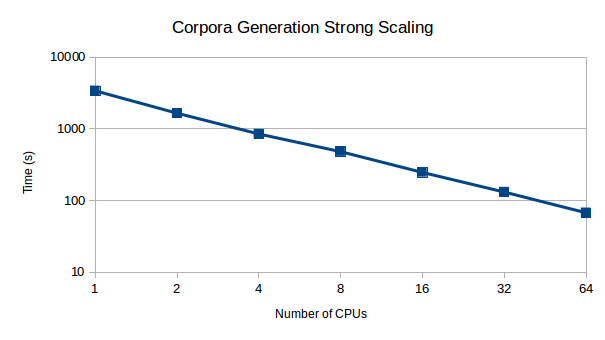
\includegraphics[width=0.49\linewidth]{Corpora_Strong_Scaling.png}}
    \hfill
  \subfloat[Tiempo de corrida vs. el número de \glspl{cpu}.\label{sub:Corpora_Weak_Scaling}]{%
	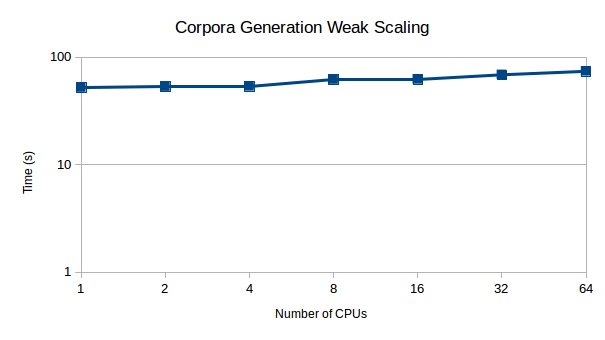
\includegraphics[width=0.49\linewidth]{Corpora_Weak_Scaling.png}}
\\
  \subfloat[Eficiencia vs. el número de \glspl{cpu}.\label{sub:Corpora_Strong_Scaling_Efficiency}]{%
       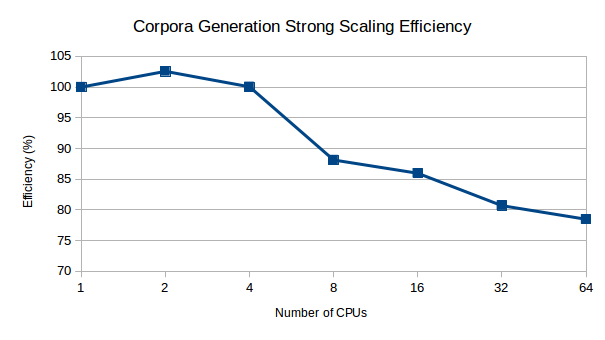
\includegraphics[width=0.49\linewidth]{Corpora_Strong_Scaling_Efficiency.png}}
    \hfill
  \subfloat[Eficiencia vs. el número de \glspl{cpu}.\label{sub:Corpora_Weak_Scaling_Efficiency}]{%
	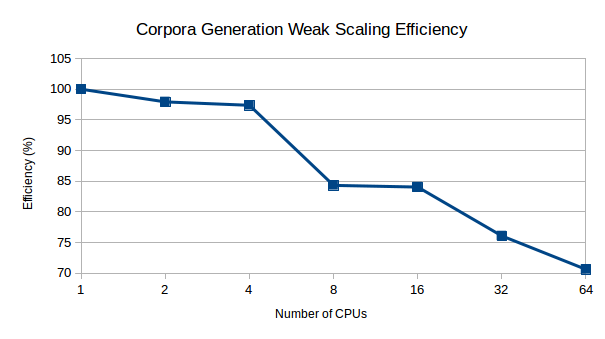
\includegraphics[width=0.49\linewidth]{Corpora_Weak_Scaling_Efficiency.png}}
	\caption{Pruebas de escalado Fuerte y Débil sobre el algoritmo de Generación de Corpus.}
  \label{fig:Corpora_Scaling} 
\end{figure*}

La línea recta en la Fig.~\ref{sub:Corpora_Strong_Scaling} muestra una buena capacidad de escalado fuerte de nuestro código.
Para las pruebas de desempeño de escalado fuerte el tamaño del problema se mantiene constante, es decir, la corrida tiene que generar 64 corpus.
Por otro lado el número de elementos de procesamiento se incrementa desde 1 a 64 \gls{cpu_pl} en potencias de dos.
En este caso corrimos un proceso \gls{mpi} por \gls{cpu}.
Debido a que un nodo en Cooley tiene 12 \gls{cpu_pl} solo necesitamos 1 nodo para correr 1, 2, 4 u 8 procesos, 2 nodos (24 \gls{cpu_pl}) para correr 16 procesos, 3 nodos (36 \gls{cpu_pl}) para correr 32 procesos y finalmente 6 nodos (72 \gls{cpu_pl}) para correr 64 procesos.

Algo a tomar en cuenta es que para hacer que este código escale de la manera que se muestra en las gráficas, todos los corpus deben tener el mismo tamaño, de otra manera--debido a que el código distribuye los corpus sobre los diferentes procesos de manera estática--algunos procesos a cargo de corpus más pequeños habrían finalizado antes que otros procesos a cargo de corpus más grandes y así habrían desperdiciado su tiempo esperando de manera inactiva por la finalización de aquellos procesos.
Por lo tanto es necesario realizar una distribución de vocabularios sobre procesos de manera dinámica--así como la planificación dinámica en \gls{omp}.
De todas maneras, tratar de balancear la carga entre los diferentes procesos \gls{mpi} podría producir una degradación severa de la Eficiencia originada en el ingremento de la carga en \gls{ipc} que tales técnicas requieren~\cite{hu2012biophysically}.

Sea $t_1$ la cantidad de tiempo requerida para completar una unidad de trabajo con $1$ elemento de procesamiento, y $t_N$ la cantidad de tiempo para completar la misma unidad de trabajo con $N$ elementos de procesamiento, la Eficiencia de Escalado Fuerte es: $t_1 / (N * t_N) * 100$. En la Fig.~\ref{sub:Corpora_Strong_Scaling_Efficiency} podemos ver que la eficiencia mínima de escalado fuerte está muy por encima del 75\%.

En referencia al escalado débil (Fig.~\ref{sub:Corpora_Weak_Scaling}) el problema de la carga de trabajo asignada a cada elemento de procesamiento se mantiene constante y se utilizan elementos adicionales para resolver problemas más grandes (es decir mientras agregamos más \glspl{cpu} también agregamos más corpus de tal manera que siempre se genere un corpus por \gls{cpu}).
Generamos un corpus por cada proceso utilizando: un corpus por proceso \gls{mpi}, dos corpus para dos procesos \gls{mpi} y así.
Sea $t_1$ la cantidad de tiempo para completar una unidad de trabajo con $1$ elemento de procesamiento, y $t_N$ la cantidad de tiempo para completar $N$ veces la misma unidad de trabajo con $N$ elementos de procesamiento, la eficiencia de escalado débil es: $t_1 / t_N * 100$. Las líneas casi horizontales mostradas en la Fig.~\ref{sub:Corpora_Weak_Scaling} ilustran que el código también escala bien en términos de escalado débil y que--como se muestra en la Fig.~\ref{sub:Corpora_Weak_Scaling_Efficiency}--la eficiencia del escalado débil del código nunca estuvo por debajo del the 70\%.
}{
\subsection{Corpora Generation Scaling Tests}
\label{CG_Scaling_test}

In terms of Strong and Weak scaling (Fig.~\ref{fig:Corpora_Scaling}), we ran the algorithm in order to create 64 corpora from 64 vocabularies--one corpus per vocabulary. The code generated 64 cross synthesizer SABLE text files and then called to Festival using \texttt{text2wav} script in order to generate the audio \texttt{wav} files which uttered the text in the SABLE files.

\begin{figure*}[tb] 
    \centering
  \subfloat[Run time vs. the number of \glspl{cpu}.\label{sub:Corpora_Strong_Scaling}]{%
       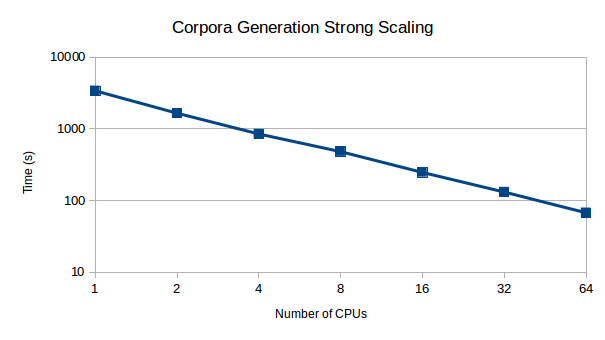
\includegraphics[width=0.49\linewidth]{Corpora_Strong_Scaling.png}}
    \hfill
  \subfloat[Run time vs. the number of \glspl{cpu}.\label{sub:Corpora_Weak_Scaling}]{%
	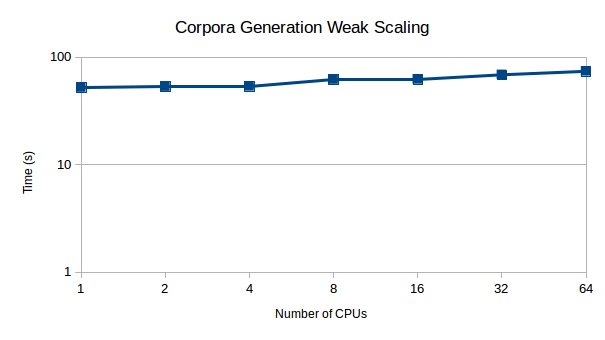
\includegraphics[width=0.49\linewidth]{Corpora_Weak_Scaling.png}}
\\
  \subfloat[Efficiency vs. the number of \glspl{cpu}.\label{sub:Corpora_Strong_Scaling_Efficiency}]{%
       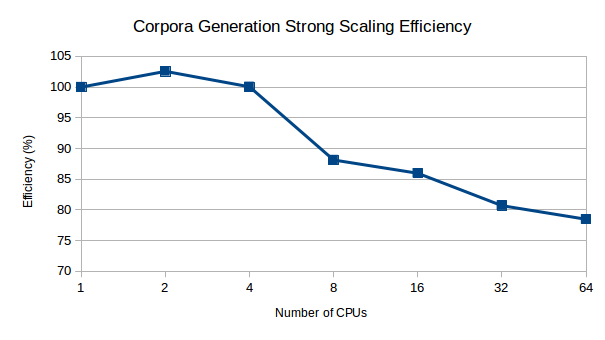
\includegraphics[width=0.49\linewidth]{Corpora_Strong_Scaling_Efficiency.png}}
    \hfill
  \subfloat[Efficiency vs. the number of \glspl{cpu}.\label{sub:Corpora_Weak_Scaling_Efficiency}]{%
	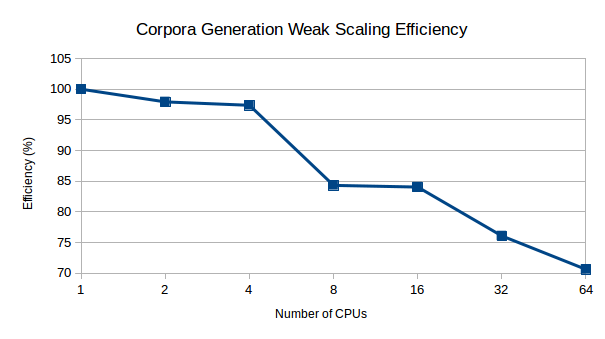
\includegraphics[width=0.49\linewidth]{Corpora_Weak_Scaling_Efficiency.png}}
	\caption{Strong and Weak scaling tests on Corpora Generation algorithm.}
  \label{fig:Corpora_Scaling} 
\end{figure*}

The straight line in Fig.~\ref{sub:Corpora_Strong_Scaling} shows a good strong scaling capacity of our code. For strong scaling performance tests the problem size stays fixed, that is, the run has to generate 64 corpora. On the other hand the number of processing elements is increased from 1 to 64 \glspl{cpu} in powers of two. In this case we ran one \gls{mpi} rank per \gls{cpu}. Since one Cooley Node has 12 \glspl{cpu} we just needed 1 node in order to run 1, 2, 4 or 8 processes, 2 nodes (24 \glspl{cpu}) in order to run 16 processes, 3 nodes (36 \glspl{cpu}) in order to run 32 processes and finally 6 nodes (72 \glspl{cpu}) in order to run 64 processes.

Something to take into account is that to make this code scale in the way shown by the chart, all the corpora must have the same size, otherwise--and since the code distributes corpora on different processes in static way--some processes which took over smaller corpora would have finished before other processes that took over larger corpora and would have wasted processing power waiting idly for other processes to finish. It is therefore necessary to make the distribution of vocabularies on processes, dynamic--such as \gls{omp} dynamic schedule. Nevertheless, trying to balance the load among the different \gls{mpi} ranks could produce a severe degradation of Efficiency originated in the increased \gls{ipc} load that such techniques require~\cite{hu2012biophysically}.

Let $t_1$ be the amount of time to complete a work unit with $1$ processing element, and $t_N$ the amount of time to complete the same unit of work with $N$ processing elements, the Strong Scaling Efficiency is: $t_1 / (N * t_N) * 100$. In Fig.~\ref{sub:Corpora_Strong_Scaling_Efficiency} we can see that the minimum Strong Scaling Efficiency is well above the 75\%.

In reference to Weak scaling (Fig.~\ref{sub:Corpora_Weak_Scaling}) the problem workload assigned to each processing element stays constant and additional elements are used to solve a larger total problem (i.e. as we add more \glspl{cpu} we add more corpora in a way that one corpus is generated per \gls{cpu}). We generated one corpus per process using one corpus for one \gls{mpi} rank, two corpora for two \gls{mpi} ranks and so on. Let $t_1$ be the amount of time to complete a work unit with $1$ processing element, and $t_N$ the amount of time to complete $N$ times the same unit of work with $N$ processing elements, the Weak Scaling Efficiency is: $t_1 / t_N * 100$. The almost horizontal line shown in Fig.~\ref{sub:Corpora_Weak_Scaling} depicts that this code scales well in terms of weak scaling too and--as Fig.~\ref{sub:Corpora_Weak_Scaling_Efficiency} shows--the Weak Scaling Efficiency of the code was never below the 70\%.
}










\iftoggle{DEBUG}{
\subsection{Pruebas de Escalado para \glsfirst{mrstsa}}
\label{MRSTSA_Scaling_Tests}

En términos de Escalado Fuerte, corremos el algoritmo para procesar 64 corpus--un corpus por vocabulario.
Las líneas rectas en la Fig.~\ref{sub:MRSTSA_Strong_Scaling} muestran un escalado muy bueno de este código.
El tamaño del problema se mantuvo constante en 64 corpus procesados por medio del algortimo \gls{mrstsa} mientras que se incrementó el número de elementos de procesamiento.

\begin{figure*}[tb] 
    \centering
  \subfloat[Tiempo de corrida vs. el número de nodos para diferentes números de hilos por nodo.\label{sub:MRSTSA_Strong_Scaling}]{%
       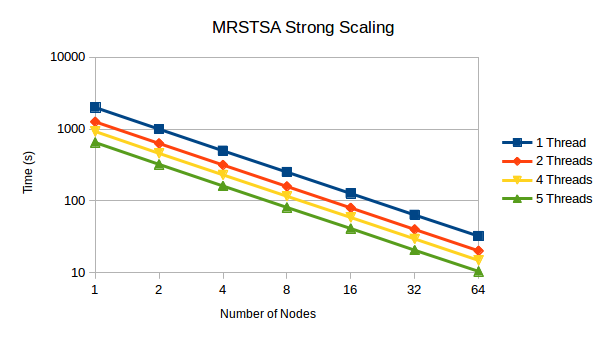
\includegraphics[width=0.49\linewidth]{MRSTSA_Strong_Scaling.png}}
    \hfill
  \subfloat[Tiempo de corrida vs. el número de nodos para 5 hilos por nodo.\label{sub:MRSTSA_Weak_Scaling}]{%
	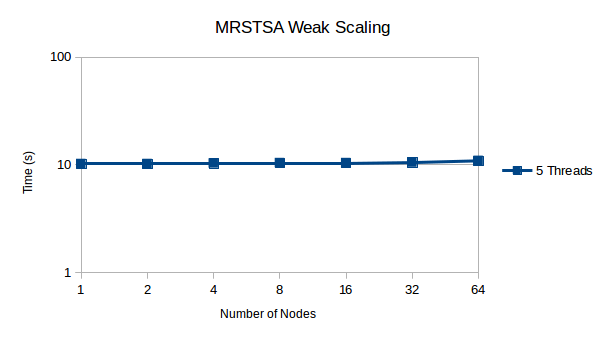
\includegraphics[width=0.49\linewidth]{MRSTSA_Weak_Scaling.png}}
\\
  \subfloat[Eficiencia vs. el número de nodos para diferentes números de hilos por nodo.\label{sub:MRSTSA_Strong_Scaling_Efficiency}]{%
       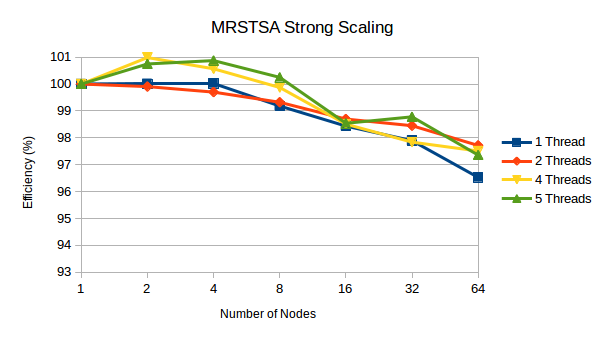
\includegraphics[width=0.49\linewidth]{MRSTSA_Strong_Scaling_Efficiency.png}}
    \hfill
  \subfloat[Eficiencia vs. el número de nodos para 5 hilos por nodo.\label{sub:MRSTSA_Weak_Scaling_Efficiency}]{%
	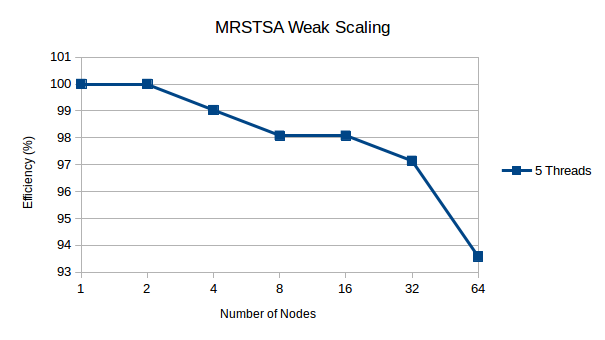
\includegraphics[width=0.49\linewidth]{MRSTSA_Weak_Scaling_Efficiency.png}}
	\caption{Pruebas de escalado Fuerte y Débil del algoritmo \gls{mrstsa} sobre los nodos de Cooley. Cada proceso \gls{mpi} corre en un nodo diferente con 1, 2, 4 y 5 hilos \gls{omp} corriendo en cada proceso.}
  \label{fig:MRSTSA_Scaling} 
\end{figure*}

Cada proceso corre en un nodo diferente. Utilizamos un número de hilos \gls{omp} cuyo rango varió de 1 a 5.
Cinco es el número de componentes espectrales en el algoritmo \gls{mrstsa}~\cite{10.1371/journal.pone.0217966}.
Como en la sección \ref{CG_Scaling_test}, un aspecto a tomar en cuenta es que para hacer que este código escale de la manera expuesta por la gráfica, todos los corpus debieron tener el mismo tamaño, de lo contrario--debido a que el código distribuye los corpus en diferentes procesos de manera estática--algunos procesos que se encarguen de corpus más pequeños habrían finalizado antes que otros procesos encargados de corpus más grandes, produciendo así un desbaance importante de la carga en el entorno \gls{mpi}.
Por lo tanto es necesario hacer que la distribución de corpus en los procesos sea dinámica--tal como la planificación dinámica en \gls{omp}.
Sin embargo, así como se expresó en la sección \ref{CG_Scaling_test}, tratar de balancear la carga entre los diferentes procesos \gls{mpi} podría producir una degradación severa de la eficiencia originada en el incremento de la carga de \gls{ipc} que tales técnicas requieren~\cite{hu2012biophysically}.

En referencia al escalado débil, procesamos un corpus por proceso \gls{mpi} por medio del procesamiento de: un corpus para un proceso \gls{mpi}, dos corpus para dos procesos \gls{mpi}, cuatro corpus para cuatro procesos \gls{mpi} y así.
En la Fig.~\ref{sub:MRSTSA_Weak_Scaling} la carga de trabajo en el problema asignada a cada elemento de procesamiento se mantuvo constante y se incorporaron elementos adicionales para resolver un problema más grande.
Incorporamos más corpus por corrida mientras el número de nodos se incrementaba de tal manera que cada nodo tuviera un corpus para procesar.
La línea horizontal en la Fig.~\ref{sub:MRSTSA_Weak_Scaling} muestra que este código escala bien en términos de escalado débil también.

Finalmente, las Figs.~\ref{sub:MRSTSA_Strong_Scaling_Efficiency} and~\ref{sub:MRSTSA_Weak_Scaling_Efficiency} sostienen el comportamiento de las gráficas con eficiencias de escalado fuerte bien arriba del 96\% y de escalado débil arriba del 93\%. 
}{
\subsection{\glsfirst{mrstsa} Scaling Tests}
\label{MRSTSA_Scaling_Tests}

In terms of Strong scaling, we ran the algorithm in order to process 64 corpora--one corpus per vocabulary. Straight lines in Fig.~\ref{sub:MRSTSA_Strong_Scaling} show a really good scaling of this code. The problem size stayed fixed in 64 corpora processed by means of \gls{mrstsa} algorithm, while the number of processing elements was increased.

\begin{figure*}[tb] 
    \centering
  \subfloat[Run time vs. the number of nodes for different number of threads per node.\label{sub:MRSTSA_Strong_Scaling}]{%
       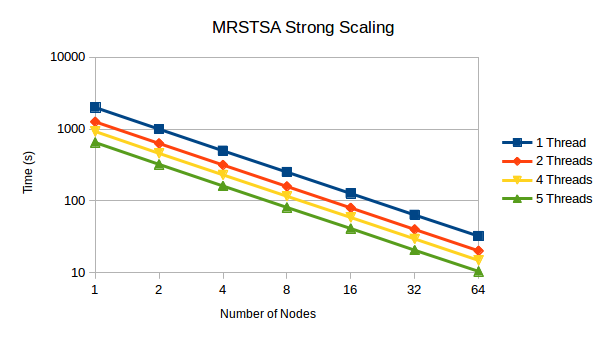
\includegraphics[width=0.49\linewidth]{MRSTSA_Strong_Scaling.png}}
    \hfill
  \subfloat[Run time vs. the number of nodes for 5 threads per node.\label{sub:MRSTSA_Weak_Scaling}]{%
        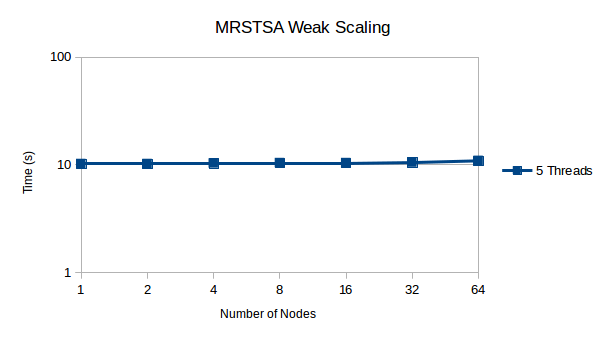
\includegraphics[width=0.49\linewidth]{MRSTSA_Weak_Scaling.png}}
\\
  \subfloat[Efficiency vs. the number of nodes for different number of threads per node.\label{sub:MRSTSA_Strong_Scaling_Efficiency}]{%
       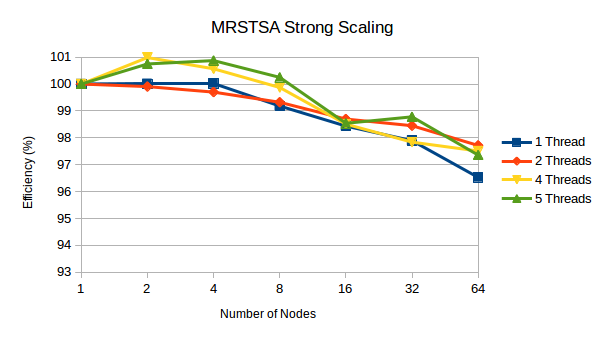
\includegraphics[width=0.49\linewidth]{MRSTSA_Strong_Scaling_Efficiency.png}}
    \hfill
  \subfloat[Efficiency vs. the number of nodes for 5 threads per node.\label{sub:MRSTSA_Weak_Scaling_Efficiency}]{%
        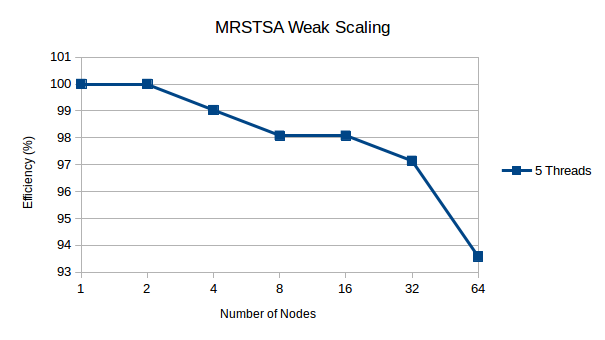
\includegraphics[width=0.49\linewidth]{MRSTSA_Weak_Scaling_Efficiency.png}}
	\caption{Strong and Weak scaling tests of the \gls{mrstsa} algorithm on Cooley nodes. Each \gls{mpi} rank runs in a different node with 1, 2, 4 and 5 \gls{omp} threads running in each rank.}
  \label{fig:MRSTSA_Scaling} 
\end{figure*}

Each process ran in a different node. We used a number of \gls{omp} threads which ranged from 1 to 5. Five is the number of spectral components in the \gls{mrstsa} algorithm~\cite{10.1371/journal.pone.0217966}. As in section \ref{CG_Scaling_test}, one aspect to take into account is that in order to make this code scale in the way shown by the chart, all the corpora must have the same size, otherwise--and since the code distributes corpora on different processes in a static way--some processes which took over smaller corpora would have finished before than other processes that took over larger corpora, thus producing considerable load imbalance in the \gls{mpi} environment. Therefore, it is necessary to make the distribution of corpora on processes, dynamic--such as \gls{omp} dynamic schedule. Nevertheless, as was pointed out in section \ref{CG_Scaling_test}, trying to balance the load among the different \gls{mpi} ranks could produce a severe degradation of Efficiency originated in the increased load of \gls{ipc} that such techniques require~\cite{hu2012biophysically}.

In reference to Weak scaling, we processed one corpus per \gls{mpi} rank by means of processing one corpus for one \gls{mpi} rank, two corpora for two \gls{mpi} ranks, four corpora for four \gls{mpi} ranks and so on. In Fig.~\ref{sub:MRSTSA_Weak_Scaling} the problem workload assigned to each processing element stayed constant and additional elements were used to solve a larger total problem. We added more corpora per run as the number of nodes increases in such a way that each node has to process only one corpus. The horizontal line in Fig.~\ref{sub:MRSTSA_Weak_Scaling} shows that this code scales very well in terms of weak scaling too.

Finally, Figs.~\ref{sub:MRSTSA_Strong_Scaling_Efficiency} and~\ref{sub:MRSTSA_Weak_Scaling_Efficiency} sustain the behavior of the charts with Strong Scaling Efficiencies well above 96\% and Weak Scaling Efficiencies above 93\%.
}




\iftoggle{DEBUG}{
\subsection{Pruebas de Escalado de la \glsfirst{el}}

La Fig. \ref{fig:EL_Strong_Scaling} muestra la capacidad de escalado fuerte de nuestro código en términos del tiempo de corrida vs. el número de elementos de procesamiento utilizados para la tarea.
En estas pruebas restringimos el código para que corra un proceso \gls{mpi} por nodo.
Cada proceso \gls{mpi} distribuye un número específico de hilos a través de las diferentes \gls{cpu_pl} en su nodo correspondiente como se muestra en la Fig. \ref{fig:Encoder_Parallelization}.
Como se mostró anteriormente, el tamaño del problema se mantuvo constante y se incrementó el número de elementos de procesamiento.
Las líneas rectas en las Figs.~\ref{sub:EL_Strong_Scaling_Left} y~\ref{sub:EL_Strong_Scaling1_Left} muestran--a primera vista--una buena capacidad de escalado.
Este hecho es respaldado por las Figs.~\ref{sub:EL_Strong_Scaling_Right} y~\ref{sub:EL_Strong_Scaling1_Right} por medio de la eficiencia de escalado fuerte: $t_1 / (N * t_N) * 100$.

\begin{figure*}[tb] 
    \centering
  \subfloat[Tiempo de corrida vs. el número de nodos para diferente números de hilos por nodo.\label{sub:EL_Strong_Scaling_Left}]{%
       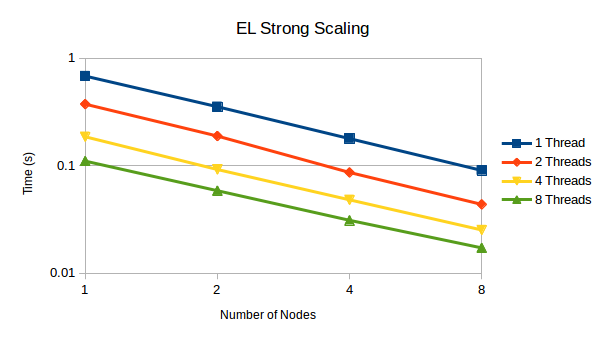
\includegraphics[width=0.49\linewidth]{EL_Strong_Scaling_Left.png}}
    \hfill
  \subfloat[Eficiencia vs. el número de nodos para diferente número de hilos por nodo.\label{sub:EL_Strong_Scaling_Right}]{%
	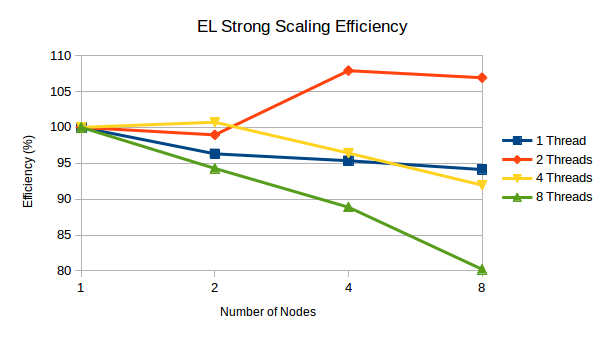
\includegraphics[width=0.49\linewidth]{EL_Strong_Scaling_Right.png}}
\\
  \subfloat[Tiempo de corrida vs. el número de nodos para diferente número de hilos por nodo.\label{sub:EL_Strong_Scaling1_Left}]{%
       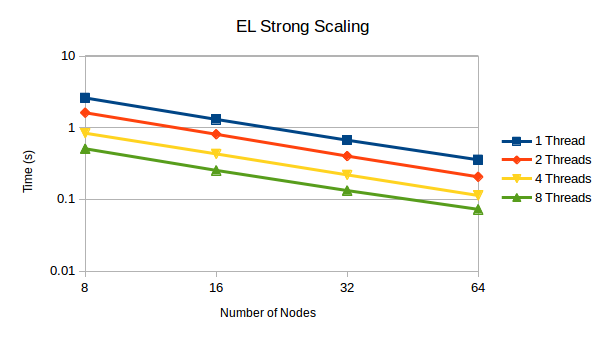
\includegraphics[width=0.49\linewidth]{EL_Strong_Scaling1_Left.png}}
    \hfill
    \subfloat[Eficiencia vs. el número de nodos para diferentes números de hilos por nodo. Referencia (Race line) se toma desde los 8 nodos computacionales.\label{sub:EL_Strong_Scaling1_Right}]{%
	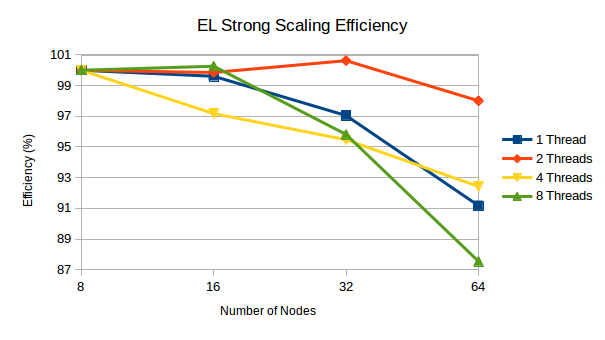
\includegraphics[width=0.49\linewidth]{EL_Strong_Scaling1_Right.png}}
	\caption{Pruebas de escalado Fuerte del algoritmo \gls{el}. Cada proceso \gls{mpi} corre en un nodo diferente con 1, 2, 4 y 8 hilos \gls{omp} corriendo en cada proceso.}
  \label{fig:EL_Strong_Scaling} 
\end{figure*}

Para las pruebas mostradas en las Figs.~\ref{sub:EL_Strong_Scaling_Left} y~\ref{sub:EL_Strong_Scaling_Right} generamos una \gls{el} cuyas especificaciones se muestran en el Cuadro~\ref{Medium_Model}, mientras que para las pruebas mostradas en las Figs.~\ref{sub:EL_Strong_Scaling1_Left} and~\ref{sub:EL_Strong_Scaling1_Right} generamos una \gls{el} cuyas especificaciones se muestran en el Cuadro~\ref{Big_Model}.

\begin{table*}[tb]
\centering
\caption{Una \gls{el} de tamaño normal para probar el escalado fuerte sobre 1, 2, 4 y 8 nodos computacionales. Los \glspl{rf} diferentes, los porcentajes y las dimensionalidades se expresan en~\cite{10.1371/journal.pone.0217966}.}
\begin{tabular}{|c|l|l|l|l|l|l|l|}
\hline
Modelo  & \multicolumn{1}{c|}{\begin{tabular}[c]{@{}c@{}}Número\\ de CCs\end{tabular}} & \multicolumn{1}{c|}{\begin{tabular}[c]{@{}c@{}}CR\\ Aferente\end{tabular}} & \multicolumn{1}{c|}{\begin{tabular}[c]{@{}c@{}}Aferente\\ \%\end{tabular}} & \multicolumn{1}{c|}{\begin{tabular}[c]{@{}c@{}}CR\\ Lateral\end{tabular}} & \multicolumn{1}{c|}{\begin{tabular}[c]{@{}c@{}}Lateral\\ \%\end{tabular}} & \multicolumn{1}{c|}{\begin{tabular}[c]{@{}c@{}}Dimensionalidad de\\ la Population\end{tabular}} & \multicolumn{1}{c|}{\begin{tabular}[c]{@{}c@{}}Potencial\\ \%\end{tabular}} \\ \hline
Normal & 23 x 23                                                                      & 5 x 127                                                                      & 5\%                                                                        & 9 x 9                                                                     & 90\%                                                                      & 15 x 15                                                                                  & 3\%                                                                         \\ \hline
\end{tabular}%}
\label{Medium_Model}
\end{table*}

En primer lugar, la \gls{el} probada en las Figs.~\ref{sub:EL_Strong_Scaling_Left} y~\ref{sub:EL_Strong_Scaling_Right} tiene 529 \gls{cc_pl}.
Para evitar la degradación en la eficiencia del escalado, la \gls{el} tiene que mantener cierto número de \gls{cc_pl} por hilo \gls{omp}.
En general, mientras más baja sea la tasa de \glspl{cc} por hilo \gls{omp}, más baja es la eficiencia medida de escalado.
El peor caso en la Fig.~\ref{sub:EL_Strong_Scaling_Left} es para 8 nodos corriendo 8 hilos cada uno (es decir, 64 hilos en total).
En tal caso terminamos teniendo aproximadamente 8,2 \gls{cc_pl} por hilo \gls{omp}.
Como se puede ver en la Fig.~\ref{sub:EL_Strong_Scaling_Right} la eficiencia de escalado fuerte nunca estuvo por debajo del 80\%.

Debido a que nuestro modelo computacional se direcciona a correr en supercomputadoras del más alto desempeño--como Theta en el \gls{alcf}--en el futuro, fue necesario probar la eficiencia de escalado fuerte del modelo en más nodos computacionales.
Especificamente queríamos probar el comportamiento del escalado corriendo con hasta 64 nodos cada uno con 8 hilos \gls{omp} ya que mientras más nodos se incorporan, más carga en \gls{ipc} se tiene.
Para mantener un número considerable de \gls{cc_pl} por  hilo \gls{omp} generamos una \gls{el} con las especificaciones mostradas en el Cuadro~\ref{Big_Model}.

\begin{table*}[tb]
\centering
\caption{Una \gls{el} de tamaño grande para pruebas de escalado fuerte sobre 8, 16, 32 y 64 nodos computacionales. Los diferentes \glspl{rf}, los porcentajes y dimensionalidades se explican en~\cite{10.1371/journal.pone.0217966}.}
\begin{tabular}{|c|l|l|l|l|l|l|l|}
\hline
Modelo  & \multicolumn{1}{c|}{\begin{tabular}[c]{@{}c@{}}Npumero\\ de CCs\end{tabular}} & \multicolumn{1}{c|}{\begin{tabular}[c]{@{}c@{}}CR\\ Aferente\end{tabular}} & \multicolumn{1}{c|}{\begin{tabular}[c]{@{}c@{}}Aferente\\ \%\end{tabular}} & \multicolumn{1}{c|}{\begin{tabular}[c]{@{}c@{}}CR\\ Lateral\end{tabular}} & \multicolumn{1}{c|}{\begin{tabular}[c]{@{}c@{}}Lateral\\ \%\end{tabular}} & \multicolumn{1}{c|}{\begin{tabular}[c]{@{}c@{}}Dimensionalidad de\\ la Población\end{tabular}} & \multicolumn{1}{c|}{\begin{tabular}[c]{@{}c@{}}Potencial\\ \%\end{tabular}} \\ \hline
Grande & 128 x 128                                                                      & 5 x 127                                                                      & 5\%                                                                        & 9 x 9                                                                     & 90\%                                                                      & 15 x 15                                                                                  & 3\%                                                                         \\ \hline
\end{tabular}%}
\label{Big_Model}
\end{table*}

Este modelo tuvo 16384 \glspl{cc} y para el peor caso en el que hubieron 64 nodos computacionales con 8 hilos \gls{omp} cada uno (512 hilos en total), el modelo terminó distribuyendo 32 \gls{cc_pl} por hilo \gls{omp}, una tasa mucho mejor que la dada para el caso anterior.
Cada \gls{cc} en este modelo tuvo 225 unidades neuronales para alcanzar un totalde 3686400 unidades neuronales.
Cada unidad neuronal tuvo 31 sinapsis próximas (aferentes) y 432 sinapsis distales (laterales) para alcanzar un total de 1706803200 sinapsis en la \gls{el}.
Dado el tamaño de este modelo no pudimos correr experimentos desde 1, 2 o 4 nodos computacionales ya que la cantidad de tiempo que una simulación de tales características puede tomar, exede por mucho el tiempo provisto por el comando \texttt{qsub} en Cooley.
Por lo tanto, comenzamos las pruebas desde 8 nodos computacionales para  1, 2, 4 y 8 hilos \gls{omp} como muestra la Fig.~\ref{sub:EL_Strong_Scaling1_Left}.

Como se puede ver en la Fig.~\ref{sub:EL_Strong_Scaling1_Right}, la mayor cantidad de nodos computacionales (procesos \gls{mpi}) con el consecuente crecimiento de la carga en \gls{ipc} \gls{mpi}, no afectó la eficiencia del escalado fuerte del modelo la cual estuvo por encima del 87\% cuando se corrieron 8 hilos por nodo, pero estuvo muy arriba del 97\% cuando se corrieron dos hilos por nodo para 64 nodos. 

En referencia al escalado débil, con el fin de mantener la tasa en el número de \glspl{cc} por hilo \gls{omp} constante, utilizamos las \gls{el_pl} detalladas en el Cuadro~\ref{Weak_Scaling_Models}.
Para todos los casos detallados en el cuadro la tasa de \gls{cc_pl} por hilo \gls{omp} fue de 32.

\begin{table*}[tb]
\centering
\caption{\glspl{el} de diferentes tamaños para probar el escalado débil sobre 1, 2, 4, 8, 16, 32 y 64 nodos computacionales. Los diferentes \glspl{rf}, porcentajes y dimensionalidades se explican en~\cite{10.1371/journal.pone.0217966}.}
\begin{tabular}{|c|c|c|c|c|c|c|c|}
\hline
\begin{tabular}[c]{@{}c@{}}Número de\\ Nodos\end{tabular} & \begin{tabular}[c]{@{}c@{}}Número\\ de CCs\end{tabular} & \begin{tabular}[c]{@{}c@{}}CR\\ Aferente\end{tabular} & \begin{tabular}[c]{@{}c@{}}Aferente\\ \%\end{tabular} & \begin{tabular}[c]{@{}c@{}}CR\\ Lateral\end{tabular} & \begin{tabular}[c]{@{}c@{}}Lateral\\ \%\end{tabular} & \begin{tabular}[c]{@{}c@{}}Dimensionalidad de\\ la Población\end{tabular} & \begin{tabular}[c]{@{}c@{}}Potencial\\ \%\end{tabular} \\ \hline
1 Nodo                                                    & 16 x 16                                                 & 5 x 127                                                 & 5\%                                                   & 9 x 9                                                & 90\%                                                 & 15 x 15                                                             & 3\%                                                    \\ \hline
2 Nodos                                                   & 16 x 32                                                 & 5 x 127                                                 & 5\%                                                   & 9 x 9                                                & 90\%                                                 & 15 x 15                                                             & 3\%                                                    \\ \hline
4 Nodos                                                   & 32 x 32                                                 & 5 x 127                                                 & 5\%                                                   & 9 x 9                                                & 90\%                                                 & 15 x 15                                                             & 3\%                                                    \\ \hline
8 Nodos                                                   & 32 x 64                                                 & 5 x 127                                                 & 5\%                                                   & 9 x 9                                                & 90\%                                                 & 15 x 15                                                             & 3\%                                                    \\ \hline
16 Nodos                                                  & 64 x 64                                                 & 5 x 127                                                 & 5\%                                                   & 9 x 9                                                & 90\%                                                 & 15 x 15                                                             & 3\%                                                    \\ \hline
32 Nodos                                                  & 64 x 128                                                & 5 x 127                                                 & 5\%                                                   & 9 x 9                                                & 90\%                                                 & 15 x 15                                                             & 3\%                                                    \\ \hline
64 Nodos                                                  & 128 x 128                                               & 5 x 127                                                 & 5\%                                                   & 9 x 9                                                & 90\%                                                 & 15 x 15                                                             & 3\%                                                    \\ \hline
\end{tabular}%}
\label{Weak_Scaling_Models}
\end{table*}

La Fig.~\ref{fig:EL_Weak_Scaling} muestra el desempeño de escalado débil del modelo.
En este caso la carga del problema signada a cada elemento de procesamiento se mantuvo constante  y se agregaron elementos adicionales para resolver un problema más grande.
Las líneas horizontales en la Fig.~\ref{sub:EL_Weak_Scaling_Left} muestran--a primera vista--un buen ecenario.
Como se puede ver en la Fig.~\ref{sub:EL_Weak_Scaling_Right}, la eficiencia de escalado estuvo siempre por arriba del 75\%, donde la eficiencia de escalado débil es: $t_1 / t_N * 100$.
Estas medidas muestran que la ejecución paralela del modelo no fue afectada por la carga \gls{ipc} \gls{mpi} cuando el número de nodos computacionales se incrementó.
Este escenario es especialmente evidente para el caso de un hilo \gls{omp} en cuyo caso la peor eficiencia está arriba del 95\%.

\begin{figure*}[tb] 
    \centering
  \subfloat[Tiempo de corrida vs. el número de nodos para diferentes números de hilos por nodo.\label{sub:EL_Weak_Scaling_Left}]{%
       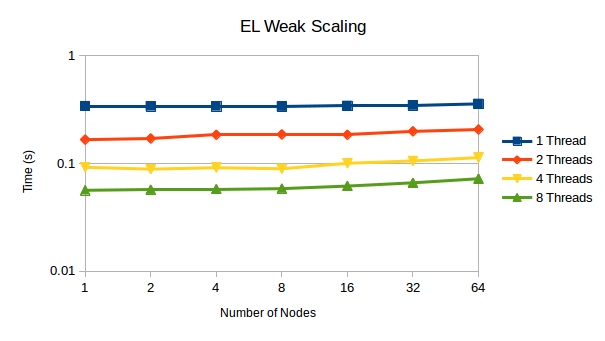
\includegraphics[width=0.49\linewidth]{EL_Weak_Scaling_Left.png}}
    \hfill
  \subfloat[Eficiencia vs. el número de nodos para diferentes números de hilos por nodo.\label{sub:EL_Weak_Scaling_Right}]{%
	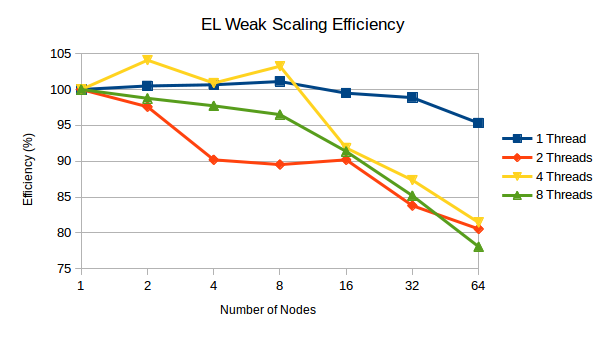
\includegraphics[width=0.49\linewidth]{EL_Weak_Scaling_Right.png}}

	\caption{Pruebas de escalado débil del algoritmo \gls{el} sobre los nodos de Cooley. Cada proceso \gls{mpi} corre en un nodo diferente con 1, 2, 4 y 8 hilos \gls{omp} corriendo en cada proceso.}
  \label{fig:EL_Weak_Scaling} 
\end{figure*}

Las Figs.~\ref{sub:EL_Strong_Scaling_Left} y~\ref{sub:EL_Strong_Scaling1_Left} muestran una escalabilidad \emph{fuerte} inicialmente buena de nuestro código miesntras que la Fig. \ref{sub:EL_Weak_Scaling_Left} nos permite vislumbrar un buen desempeño en escalabilidad \emph{débil} en supercomputadoras de alto desempeño también.
Todos esos resultados visuales son sostenidos por buenas medidas de eficiencia.
}{
\subsection{\glsfirst{el} Scaling Tests}

Fig. \ref{fig:EL_Strong_Scaling} shows the strong scaling capacity of our code in terms of run time vs. number of processing elements used for the task. In these tests we constrained the code to run one \gls{mpi} rank per node. Each \gls{mpi} rank spread a specific number of threads through the different \glspl{cpu} in its corresponding node as shown in Fig. \ref{fig:Encoder_Parallelization}. As before, the problem size stayed fixed and the number of processing elements was increased. Straight lines in Figs.~\ref{sub:EL_Strong_Scaling_Left} and~\ref{sub:EL_Strong_Scaling1_Left} show--at first--a good scaling capacity. Such fact is supported by Figs.~\ref{sub:EL_Strong_Scaling_Right} and~\ref{sub:EL_Strong_Scaling1_Right} by means of the strong scaling efficiency: $t_1 / (N * t_N) * 100$.

\begin{figure*}[tb] 
    \centering
  \subfloat[Run time vs. the number of nodes for different number of threads per node.\label{sub:EL_Strong_Scaling_Left}]{%
       \includegraphics[width=0.49\linewidth]{EL_Strong_Scaling_Left.png}}
    \hfill
  \subfloat[Efficiency vs. the number of nodes for different numbers of threads per node.\label{sub:EL_Strong_Scaling_Right}]{%
        \includegraphics[width=0.49\linewidth]{EL_Strong_Scaling_Right.png}}
\\
  \subfloat[Run time vs. the number of nodes for different number of threads per node.\label{sub:EL_Strong_Scaling1_Left}]{%
       \includegraphics[width=0.49\linewidth]{EL_Strong_Scaling1_Left.png}}
    \hfill
    \subfloat[Efficiency vs. the number of nodes for different numbers of threads per node. Race line (reference) is taken at 8 computing nodes.\label{sub:EL_Strong_Scaling1_Right}]{%
        \includegraphics[width=0.49\linewidth]{EL_Strong_Scaling1_Right.png}}
	\caption{Strong scaling tests of the \gls{el} algorithm. Each \gls{mpi} rank runs in a different node with 1, 2, 4 and 8 \gls{omp} threads running in each rank.}
  \label{fig:EL_Strong_Scaling} 
\end{figure*}

For the tests shown in Figs.~\ref{sub:EL_Strong_Scaling_Left} and~\ref{sub:EL_Strong_Scaling_Right} we generated an \gls{el} whose specifications are shown in Table~\ref{Medium_Model}, while for the tests shown in Figs.~\ref{sub:EL_Strong_Scaling1_Left} and~\ref{sub:EL_Strong_Scaling1_Right} we generated an \gls{el} whose specifications are shown in Table~\ref{Big_Model}.

\begin{table*}[tb]
\centering
\caption{\gls{el} of normal size to test strong scaling on 1, 2, 4 and 8 computing nodes. The different \glspl{rf}, percentages and dimensionalities are explained in~\cite{10.1371/journal.pone.0217966}.}
\begin{tabular}{|c|l|l|l|l|l|l|l|}
\hline
Model  & \multicolumn{1}{c|}{\begin{tabular}[c]{@{}c@{}}Number\\ of CCs\end{tabular}} & \multicolumn{1}{c|}{\begin{tabular}[c]{@{}c@{}}Afferent\\  RF\end{tabular}} & \multicolumn{1}{c|}{\begin{tabular}[c]{@{}c@{}}Afferent\\ \%\end{tabular}} & \multicolumn{1}{c|}{\begin{tabular}[c]{@{}c@{}}Lateral\\ RF\end{tabular}} & \multicolumn{1}{c|}{\begin{tabular}[c]{@{}c@{}}Lateral\\ \%\end{tabular}} & \multicolumn{1}{c|}{\begin{tabular}[c]{@{}c@{}}Population\\ Dimensionality\end{tabular}} & \multicolumn{1}{c|}{\begin{tabular}[c]{@{}c@{}}Potential\\ \%\end{tabular}} \\ \hline
Normal & 23 x 23                                                                      & 5 x 127                                                                      & 5\%                                                                        & 9 x 9                                                                     & 90\%                                                                      & 15 x 15                                                                                  & 3\%                                                                         \\ \hline
\end{tabular}%}
\label{Medium_Model}
\end{table*}

Firstly, the \gls{el} tested in Figs.~\ref{sub:EL_Strong_Scaling_Left} and~\ref{sub:EL_Strong_Scaling_Right} has 529 \glspl{cc}. In order to avoid scaling efficiency degradation, the \gls{el} has to keep certain number of \glspl{cc} per \gls{omp} thread. In general, the lower the rate of \glspl{cc} per \gls{omp} thread, the lower the scaling efficiency measured. The worst case in Fig.~\ref{sub:EL_Strong_Scaling_Left} is for 8 nodes running 8 threads each (i.e. 64 threads). In such case we ended up having approximately 8.2 \glspl{cc} per \gls{omp} thread. As can be seen in Fig.~\ref{sub:EL_Strong_Scaling_Right} the strong scaling efficiency was never below 80\%. 

Since our computational model is intended to run on leadership supercomputers--such as Theta at \gls{alcf}--in the future, it was necessary to test the Strong Scaling Efficiency of this on more computing nodes. Specifically, we wanted to test the behaviour of the scaling running on up to 64 nodes with 8 \gls{omp} threads each since the more nodes you incorporate, the more \gls{ipc} load you have. In order to keep a considerable number of computing nodes per \gls{omp} thread we generated an \gls{el} with the specifications shown in Table~\ref{Big_Model}. 

\begin{table*}[tb]
\centering
\caption{\gls{el} of large size to test strong scaling on 8, 16, 32 and 64 computing nodes. The different \glspl{rf}, percentages and dimensionalities are explained in~\cite{10.1371/journal.pone.0217966}.}
\begin{tabular}{|c|l|l|l|l|l|l|l|}
\hline
Model  & \multicolumn{1}{c|}{\begin{tabular}[c]{@{}c@{}}Number\\ of CCs\end{tabular}} & \multicolumn{1}{c|}{\begin{tabular}[c]{@{}c@{}}Afferent\\  RF\end{tabular}} & \multicolumn{1}{c|}{\begin{tabular}[c]{@{}c@{}}Afferent\\ \%\end{tabular}} & \multicolumn{1}{c|}{\begin{tabular}[c]{@{}c@{}}Lateral\\ RF\end{tabular}} & \multicolumn{1}{c|}{\begin{tabular}[c]{@{}c@{}}Lateral\\ \%\end{tabular}} & \multicolumn{1}{c|}{\begin{tabular}[c]{@{}c@{}}Population\\ Dimensionality\end{tabular}} & \multicolumn{1}{c|}{\begin{tabular}[c]{@{}c@{}}Potential\\ \%\end{tabular}} \\ \hline
Big & 128 x 128                                                                      & 5 x 127                                                                      & 5\%                                                                        & 9 x 9                                                                     & 90\%                                                                      & 15 x 15                                                                                  & 3\%                                                                         \\ \hline
\end{tabular}%}
\label{Big_Model}
\end{table*}

This model had 16384 \glspl{cc} and for the worst case in which there were 64 computing nodes with 8 \gls{omp} threads each (512 threads), the model ended up distributing 32 \glspl{cc} per \gls{omp} thread, a much better rate than the one given in the previous case. Each \gls{cc} in this model had 225 neural units to reach a total of 3686400 neural units. Each neural unit had 31 proximal (afferent) synapses and 432 distal (lateral) synapses to reach a total of 1706803200 synapses in the \gls{el}. Given the size of this model we could not run experiments from 1, 2 nor 4 computing nodes since the amount of time a simulation of such characteristics could take, far exceeded the time provided by \texttt{qsub} command on Cooley. Therefore, we started the tests from 8 computing nodes for 1, 2, 4 and 8 \gls{omp} threads as shown in Fig.~\ref{sub:EL_Strong_Scaling1_Left}.

As can be seen in Fig.~\ref{sub:EL_Strong_Scaling1_Right}, the larger amount of computing nodes (\gls{mpi} ranks) with the consequent growth of \gls{mpi} \gls{ipc} load did not affect the strong scaling efficiency of the model which was well above 87\% when running 8 threads per node, but was even well above 97\% when running two threads per node for 64 nodes.

In reference to Weak Scaling, in order to keep the number of \glspl{cc} per \gls{omp} thread ratio constant we used the \glspl{el} detailed in the Table~\ref{Weak_Scaling_Models}. For all the cases detailed in the table, the ratio of \glspl{cc} per \gls{omp} thread was 32.

\begin{table*}[tb]
\centering
\caption{\glspl{el} of different sizes to test weak scaling on 1, 2, 4, 8, 16, 32 and 64 computing nodes. The different \glspl{rf}, percentages and dimensionalities are explained in~\cite{10.1371/journal.pone.0217966}.}
\begin{tabular}{|c|c|c|c|c|c|c|c|}
\hline
\begin{tabular}[c]{@{}c@{}}Number of\\ Nodes\end{tabular} & \begin{tabular}[c]{@{}c@{}}Number\\ of CCs\end{tabular} & \begin{tabular}[c]{@{}c@{}}Afferent\\  RF\end{tabular} & \begin{tabular}[c]{@{}c@{}}Afferent\\ \%\end{tabular} & \begin{tabular}[c]{@{}c@{}}Lateral\\ RF\end{tabular} & \begin{tabular}[c]{@{}c@{}}Lateral\\ \%\end{tabular} & \begin{tabular}[c]{@{}c@{}}Population\\ Dimensionality\end{tabular} & \begin{tabular}[c]{@{}c@{}}Potential\\ \%\end{tabular} \\ \hline
1 Node                                                    & 16 x 16                                                 & 5 x 127                                                 & 5\%                                                   & 9 x 9                                                & 90\%                                                 & 15 x 15                                                             & 3\%                                                    \\ \hline
2 Nodes                                                   & 16 x 32                                                 & 5 x 127                                                 & 5\%                                                   & 9 x 9                                                & 90\%                                                 & 15 x 15                                                             & 3\%                                                    \\ \hline
4 Nodes                                                   & 32 x 32                                                 & 5 x 127                                                 & 5\%                                                   & 9 x 9                                                & 90\%                                                 & 15 x 15                                                             & 3\%                                                    \\ \hline
8 Nodes                                                   & 32 x 64                                                 & 5 x 127                                                 & 5\%                                                   & 9 x 9                                                & 90\%                                                 & 15 x 15                                                             & 3\%                                                    \\ \hline
16 Nodes                                                  & 64 x 64                                                 & 5 x 127                                                 & 5\%                                                   & 9 x 9                                                & 90\%                                                 & 15 x 15                                                             & 3\%                                                    \\ \hline
32 Nodes                                                  & 64 x 128                                                & 5 x 127                                                 & 5\%                                                   & 9 x 9                                                & 90\%                                                 & 15 x 15                                                             & 3\%                                                    \\ \hline
64 Nodes                                                  & 128 x 128                                               & 5 x 127                                                 & 5\%                                                   & 9 x 9                                                & 90\%                                                 & 15 x 15                                                             & 3\%                                                    \\ \hline
\end{tabular}%}
\label{Weak_Scaling_Models}
\end{table*}

Fig.~\ref{fig:EL_Weak_Scaling} shows the weak scaling performance of the model. In this case the problem workload assigned to each processing element stayed constant and additional elements were used to solve a larger total problem. The horizontal lines in Fig.~\ref{sub:EL_Weak_Scaling_Left} show--at first--a good scenario. As can be seen in Fig.~\ref{sub:EL_Weak_Scaling_Right}, the scaling efficiency was always above the 75\%, where the Weak Scaling Efficiency is: $t_1 / t_N * 100$. These measures show that the model parallel execution was not affected by \gls{mpi} \gls{ipc} load as the number of computing nodes increased. This scenario is specially evident for the case of one \gls{omp} thread in whose case the worst efficiency is above 95\%.

\begin{figure*}[tb] 
    \centering
  \subfloat[Run time vs. the number of nodes for different number of threads per node.\label{sub:EL_Weak_Scaling_Left}]{%
       \includegraphics[width=0.49\linewidth]{EL_Weak_Scaling_Left.png}}
    \hfill
  \subfloat[Efficiency vs. the number of nodes for different numbers of threads per node.\label{sub:EL_Weak_Scaling_Right}]{%
        \includegraphics[width=0.49\linewidth]{EL_Weak_Scaling_Right.png}}

	\caption{Weak scaling tests of the \gls{el} algorithm on Cooley nodes. Each \gls{mpi} rank runs in a different node with 1, 2, 4 and 8 \gls{omp} threads running in each rank.}
  \label{fig:EL_Weak_Scaling} 
\end{figure*}

Figs.~\ref{sub:EL_Strong_Scaling_Left} and~\ref{sub:EL_Strong_Scaling1_Left} show an initially good strong scalability of our code while Fig. \ref{sub:EL_Weak_Scaling_Left} allows us to foresee a good weak scaling performance in high end leadership supercomputers too. All those visual results are supported by good measures of efficiency.
}











\iftoggle{DEBUG}{
\section{Discusión}

En este trabajo mostramos cómo estrategias específicas de paralelización con gran independencia de la coalescencia de los datos escalan eficientemente en sistemas de memoria distribuida mientras corren modelos computacionales biológicamente inspirados con perfiles de conectividad altamente dispersos y aleatorios.

Las implementaciones algorítmicas fuertemente basadas en arquitecturas de computación paralela \emph{\gls{simd}} imponen restricciones importantes sobre el alineamiento de los datos en memoria.
Los hilos \gls{omp} en sistemas de memoria compartida son en cambio abstracciones altamente independientes y poderosas de procesamiento que pueden realizar tareas complejas con optimizaciones eventuales de vectorización cuando sea posible.

Nuestros hallazgos muestran que las estrategias de paralelización utilizadas en este trabajo presentan una eficiencia de escalabilidad buena y robusta aún frente a cargas intensivas de \gls{ipc}.
Tal comportamiento se puede mantener de manera sostenida siempre y cuando se conserve un balance de carga computacional mínimo entre los diferentes hilos.
En la sección~\ref{MRSTSA_Scaling_Tests} mostramos eficiencias de escalado muy altas.
Aún así advertimos acerca de las dificultades de cara a un contexto con tamaños disímiles de corpus.
Alcanzar balance en la carga en sistemas de memoria distribuida es extremadamente caro dada la cantidad de sobrecarga de \gls{ipc} requerida.
De esta forma, afirmamos que la mejor manera de balancear la carga computacional entre los elementos computacionales is tratar de confinar tanta carga computacional como sea posible en una unidad de memoria compartida sin exceder las capacidades de hilado concurrente o hiper-hilado provistas por un nodo.
Una vez que se satisfacen tales condiciones se hace relativamente simple lanzar un cierto número de hilos en los que se puede distribuir el trabajo.
Ya en un sistema de memoria compartida, los hilos \gls{omp} son mucho más ligeros que los procesos \gls{mpi}, ya que los hilos no duplican el \emph{heap} ni el programa y no necesitan métodos complejos de comunicación para compartir los datos.
Asimismo, los hilos \gls{omp} pueden manejar el balance de la carga de manera eficiente y automáticamente ya que \gls{omp} maneja planificación paralela dinámica de manera autónoma.
Esto es muy deseable, especialmente en un entorno de simulación en el que los módulos individuales--como las \gls{cc_pl} en nuestro modelo cortical--no son uniformemente análogos en términos de tamaño ni conectividad.
En \gls{mpi} en cambio, el programador se tiene que hacer cargo del balanceo de la carga utilizando \gls{ipc} de manera intensiva especialmente cuando la comunicación es entre procesos en nodos diferentes.
Por otro lado los hilos \gls{omp} sufren el fenómeno denominado \emph{false shearing} en las caches de las \gls{cpu_pl}, pero con un esquema de paralelización altamente flexible como el utilizado en la sección \ref{EL_Parallelization} el usuario puede variar la granularidad en la paralelización de manera flexible para alcanzar el mejor desempeño evitando que cada hilo exceda la cuota de memoria cache disponible en cada \gls{cpu}.

En las Figs.~\ref{fig:Corpora_Scaling}, \ref{fig:MRSTSA_Scaling}, \ref{fig:EL_Strong_Scaling} y \ref{fig:EL_Weak_Scaling} el fenómeno de \emph{super-linear speedup} se hace presente en varios casos.
En S. Ristov et al. \cite{7733347} los autores afirmaron que: \texttt{la mejora super-lineal en el desempeño en algoritmos persistentes ocurre principalmente debido al incremento de recursos de cache en arquitecturas de computadoras paralelas, el precargado de variables compartidas en la organización de memoria compartida, o una mejor planificación en entornos heterogéneos.
Los efectos de las arquitecturas de memoria compartida también impactan el desempeño del comportamiento de los algoritmos granulares y escalares.}
Nosotros apoyamos dicha moción y la consideramos una explicación general y válida para nuestro caso. Sin embargo, también consideramos que se requerirá un análisis más profundo de la utilización de la memoria haciendo uso de herramientas de profiling que se podrían requerir en el futuro.

En la sectión~\ref{EL_Parallelization} podrían surgir algunos problemas cuando una única \gls{cc} es muy grande para compartir un nodo computacional con muchas otras.
Si solo 2 \gls{cc_pl} entraran en un nodo, la granularidad en la paralelización sería muy pobre, pero los hilos \gls{omp} son altamente versátiles y pueden fácilmente  manejar hilado anidado.
En tal caso podríamos variar la granularidad de paralelización de manera extremadamente accesible con todas las ventajas de \gls{omp} en términos de balance de carga dinámica.
Esta estrategia de paralelización anidada se podría aplicar en la sección~\ref{MRSTSA_Scaling_Tests} de cara a un eventual desbalance de la carga computacional desde una distribución inequitativa del tamaño de los corpus.

Este escenario en el que la carga computacional asignada a cada sistema de memoria compartida es distribuido entre un conjunto de hilos \gls{omp} altamente livianos, flexibles y dinámicos es muy favorable en un contexto en el cual el número de \gls{cpu_pl} compartiendo memoria se incrementa año tras año especialmente en computadoras de alto desempeño.
A tal efecto y de cara a los buenos resultados devueltos por nuestros experimentos, evaluamos la implementación de estas estrategias de paralelización como válidas en supercomputadoras de alto desempeño en el futuro.

Afirmamos por lo tanto que este trabajo introduce estrategias de paralelización cuya flexibilidad y robustez son particularmente útiles en escenarios científicos computacionales ampliamente variables y biológicamente inspirados cuyos enfoques de modelización pueden variar dramáticamente en estrategias de implementación biológicamente precisas diferentes en las cuales hay estructuras de redes erráticas con perfiles de conectividad altamente dispersos y aleatorios.
}{
\section{Discussion}

In this paper we show how parallelization strategies with great independence on data coalescence scale efficiently on distributed memory systems while running biologically inspired computational models with highly sparse and random connectivity profiles.

Algorithmic implementations strongly based on \gls{simd} parallel computing architectures, impose important restrictions on memory data alignment. \gls{omp} threads in shared memory systems are instead highly independent and powerful processing abstractions which can perform complex task with eventual vectorization optimizations when possible.

Our findings show that the parallelization strategies used in this work present good and robust scaling efficiency even in the face of intensive \gls{ipc} loads. Such behavior can be kept in a sustained manner as long as a minimum of balance in the computational load among different threads remains. In section~\ref{MRSTSA_Scaling_Tests} we showed very high scaling efficiencies. Yet, we warned about difficulties in the face of a context with uneven corpus sizes. Achieving load balance in distributed memory systems is extremely expensive given the amount of \gls{ipc} overload needed. In this manner, we claim that the best way to balance computational load among computing elements is to try to confine as much computational load as possible in a shared memory unit without far exceeding the concurrent threading or hyperthreading capacity provided by a node. Once such conditions are satisfied it is relatively straightforward to spawn a number of threads in which the work could be distributed. Once in a shared memory system, \gls{omp} threads are much lighter than \gls{mpi} processes, since threads do not duplicate heap nor program and they do not need complex communication methods to share data. Furthermore, \gls{omp} threads can manage load balancing efficiently and automatically since \gls{omp} manages dynamic parallel schedule on its own. This is highly desirable, specially in a simulation environment in which individual modules--such as \glspl{cc} in our cortical model--are not uniformly analogous in terms of size and or connectivity. In \gls{mpi} instead, the programmer has to deal with load balancing using intensive \gls{ipc} which is highly expensive especially when the communication is carried out among processes in different nodes. On the other side \gls{omp} threads suffer from false shearing in the \glspl{cpu} caches, but with a highly flexible parallelization scheme as the one used in section \ref{EL_Parallelization} the user can flexibly vary the parallelization granularity as to achieve the best performance avoiding that each thread exceeds the quota of cache memory available in each \gls{cpu}.

In Figs.~\ref{fig:Corpora_Scaling}, \ref{fig:MRSTSA_Scaling}, \ref{fig:EL_Strong_Scaling} and \ref{fig:EL_Weak_Scaling} the phenomenon of \emph{super-linear} speedup is present for several cases. In \cite{7733347} the authors pointed out that: \textit{ The superlinear speedup performance in persistent algorithms occurs mainly due to the increased cache resources in the parallel computer architectures, the prefetching of shared variables in shared memory organization, or better scheduling in heterogeneous environments. The effects of the shared memory architectures also impact the performance behavior of the granular and scalable algorithms}. We absolutely endorse such statement and consider it sustainable as a general explanation for our case. Nevertheless, we also consider that more in depth analysis of memory utilization using profiling tools will be needed in the future.  

In section~\ref{EL_Parallelization} some problems could arise when a single \gls{cc} is too large to share a computing node with many others. If just 2 \glspl{cc} could fit in a node, the parallelization granularity would be very poor, but \gls{omp} is highly versatile and can easily manage nested threading. In such case we could vary the parallelization granularity in an extremely accessible manner with all the advantages of \gls{omp} in terms of dynamic load balancing. This nested parallelization strategy could be applied in section~\ref{MRSTSA_Scaling_Tests} in the face of an eventual unbalanced computational load from an uneven corpora size distribution. 

This scenario in which the computational burden assigned to each shared memory system is distributed among a set of highly lightweight, flexible and dynamic \gls{omp} threads is really favorable in a context in which the number of \glspl{cpu} shearing memory increases specially in high-end supercomputers. In such respect and in teh face of the good results returned by our experiments, we evaluate as viable the implementation of these parallelization strategies in high end supercomputers in the future.

We claim thus that this work introduces parallelization strategies whose flexibility and robustness are particularly useful in overly variable and biologically inspired computational scientific scenarios whose modelization approaches can vary dramatically in different biologically accurate implementations strategies in which there are erratic network structures with highly sparse and random connectivity profiles.
}







\iftoggle{DEBUG}{
\section{Conclusión}

En este trabajo mostramos una estrategia de paralelización híbrida \gls{mpi}+\gls{omp} que escala eficientemente en un sistema de memoria distribuida corriendo un enfoque computacional inspirado en la biología de la corteza de los mamíferos con un perfil de conectividad altamente disperso e irregular.
Mostramos esta eficiencia por medio de pruebas de escalado fuerte y débil en los nodos de Cooley.

La independencia de la coalescencia de los datos, la reconfiguración flexible de la granularidad, el balanceo de carga dinámicamente planificado y el procesamiento paralelo liviano en porciones de memoria compartida configuran los rasgos sobresalientes en nuestro enfoque de paralelización.

Consideramos tales características de fundamental importancia para el uso de este procedimiento de paralelización en escenarios científicos computacionales altamente variables con conjuntos de datos irregularmente estructurados hallados de manera típica en enfoques de investigación biológicamente inspirados.

Por medio de los resultados devueltos en esta rueda de pruebas estimamos la política de paralelización aquí presentada, viable para ser usada en supercomputadoras de gran desempeño en el futuro.
}{
\section{Conclusion}

In this paper we showed a hybrid \gls{mpi}+\gls{omp} parallelization strategy which scales efficiently in a distributed memory system while running a computational approach inspired in the biology of mammalian cortex with a highly sparse and irregular connectivity profile. We showed this efficiency by means of strong and weak scaling tests at Cooley nodes.

Independence of data coalescence, flexible granularity reconfiguration, dynamically scheduled load balancing and lightweight parallel processing at shared memory parcels, configured salient features in our parallelization approach.

We consider such features of fundamental importance for the usage of this parallelization procedure in highly variable computational scientific scenarios with irregularly structured datasets typically found in biologically inspired research approaches.

By means of the results returned by this round of tests, we esteem this parallelization policy as viable to be used in high-end leadership supercomputers in the future.
}
